\documentclass{article} % For LaTeX2e
% if you need to pass options to natbib, use, e.g.:
%\PassOptionsToPackage{numbers, compress}{natbib}

\usepackage[utf8]{inputenc} % allow utf-8 input
\usepackage[T1]{fontenc}    % use 8-bit T1 fonts
\usepackage{hyperref}       % hyperlinks
\usepackage{url}            % simple URL typesetting
\usepackage{booktabs}       % professional-quality tables
\usepackage{amsfonts}       % blackboard math symbols
\usepackage{nicefrac}       % compact symbols for 1/2, etc.
\usepackage{microtype}      % microtypography
\usepackage{graphicx}
\usepackage{subcaption}

% hyperref makes hyperlinks in the resulting PDF.
% If your build breaks (sometimes temporarily if a hyperlink spans a page)
% please comment out the following usepackage line and replace
% \usepackage{icml2020} with \usepackage[nohyperref]{icml2020} above.
\usepackage{hyperref}

% Attempt to make hyperref and algorithmic work together better:
\newcommand{\theHalgorithm}{\arabic{algorithm}}


% Use the following line for the initial blind version submitted for review:
% \usepackage{icml2020}

% If accepted, instead use the following line for the camera-ready submission:
\usepackage[accepted]{icml2020}

\icmltitlerunning{\METHOD: State-Covering Self-Supervised Reinforcement Learning}

%%%%% NEW MATH DEFINITIONS %%%%%

\usepackage{amsmath,amsfonts,bm}
\usepackage{dsfont}

% Mark sections of captions for referring to divisions of figures
\newcommand{\figleft}{{\em (Left)}}
\newcommand{\figcenter}{{\em (Center)}}
\newcommand{\figright}{{\em (Right)}}
\newcommand{\figtop}{{\em (Top)}}
\newcommand{\figbottom}{{\em (Bottom)}}
\newcommand{\captiona}{{\em (a)}}
\newcommand{\captionb}{{\em (b)}}
\newcommand{\captionc}{{\em (c)}}
\newcommand{\captiond}{{\em (d)}}

% Highlight a newly defined term
\DeclareOldFontCommand{\bf}{\normalfont\bfseries}{\mathbf}
\newcommand{\newterm}[1]{{\bf #1}}


% Figure reference, lower-case.
\def\figref#1{figure~\ref{#1}}
% Figure reference, capital. For start of sentence
\def\Figref#1{Figure~\ref{#1}}
\def\twofigref#1#2{figures \ref{#1} and \ref{#2}}
\def\quadfigref#1#2#3#4{figures \ref{#1}, \ref{#2}, \ref{#3} and \ref{#4}}
% Section reference, lower-case.
\def\secref#1{section~\ref{#1}}
% Section reference, capital.
\def\Secref#1{Section~\ref{#1}}
% Reference to two sections.
\def\twosecrefs#1#2{sections \ref{#1} and \ref{#2}}
% Reference to three sections.
\def\secrefs#1#2#3{sections \ref{#1}, \ref{#2} and \ref{#3}}
% Reference to an equation, lower-case.
\def\eqref#1{equation~\ref{#1}}
% Reference to an equation, upper case
\def\Eqref#1{Equation~\ref{#1}}
% A raw reference to an equation---avoid using if possible
\def\plaineqref#1{\ref{#1}}
% Reference to a chapter, lower-case.
\def\chapref#1{chapter~\ref{#1}}
% Reference to an equation, upper case.
\def\Chapref#1{Chapter~\ref{#1}}
% Reference to a range of chapters
\def\rangechapref#1#2{chapters\ref{#1}--\ref{#2}}
% Reference to an algorithm, lower-case.
\def\algref#1{algorithm~\ref{#1}}
% Reference to an algorithm, upper case.
\def\Algref#1{Algorithm~\ref{#1}}
\def\twoalgref#1#2{algorithms \ref{#1} and \ref{#2}}
\def\Twoalgref#1#2{Algorithms \ref{#1} and \ref{#2}}
% Reference to a part, lower case
\def\partref#1{part~\ref{#1}}
% Reference to a part, upper case
\def\Partref#1{Part~\ref{#1}}
\def\twopartref#1#2{parts \ref{#1} and \ref{#2}}

\def\ceil#1{\lceil #1 \rceil}
\def\floor#1{\lfloor #1 \rfloor}
\def\1{\bm{1}}
\newcommand{\train}{\mathcal{D}}
\newcommand{\valid}{\mathcal{D_{\mathrm{valid}}}}
\newcommand{\test}{\mathcal{D_{\mathrm{test}}}}

\def\eps{{\epsilon}}


% Random variables
\def\rtau{{\bm{\tau}}}
\def\rtaup{{\bm{\tau'}}}
\def\reta{{\bm{\eta}}}
\def\ra{{\bm{a}}}
\def\rb{{\bm{b}}}
\def\rc{{\bm{c}}}
\def\rd{{\bm{d}}}
\def\re{{\bm{e}}}
\def\rf{{\bm{f}}}
\def\rg{{\bm{g}}}
\def\rh{{\bm{h}}}
\def\ri{{\bm{i}}}
\def\rj{{\bm{j}}}
\def\rk{{\bm{k}}}
\def\rl{{\bm{l}}}
% rm is already a command, just don't name any random variables m
\def\rn{{\bm{n}}}
\def\ro{{\bm{o}}}
\def\rp{{\bm{p}}}
\def\rq{{\bm{q}}}
\def\rr{{\bm{r}}}
\def\rs{{\bm{s}}}
\def\rt{{\bm{t}}}
\def\ru{{\bm{u}}}
\def\rv{{\bm{v}}}
\def\rw{{\bm{w}}}
\def\rx{{\bm{x}}}
\def\ry{{\bm{y}}}
\def\rz{{\bm{z}}}

% Random vectors
\def\rvepsilon{{\mathbf{\epsilon}}}
\def\rvtheta{{\mathbf{\theta}}}
\def\rva{{\mathbf{a}}}
\def\rvb{{\mathbf{b}}}
\def\rvc{{\mathbf{c}}}
\def\rvd{{\mathbf{d}}}
\def\rve{{\mathbf{e}}}
\def\rvf{{\mathbf{f}}}
\def\rvg{{\mathbf{g}}}
\def\rvh{{\mathbf{h}}}
\def\rvu{{\mathbf{i}}}
\def\rvj{{\mathbf{j}}}
\def\rvk{{\mathbf{k}}}
\def\rvl{{\mathbf{l}}}
\def\rvm{{\mathbf{m}}}
\def\rvn{{\mathbf{n}}}
\def\rvo{{\mathbf{o}}}
\def\rvp{{\mathbf{p}}}
\def\rvq{{\mathbf{q}}}
\def\rvr{{\mathbf{r}}}
\def\rvs{{\mathbf{s}}}
\def\rvt{{\mathbf{t}}}
\def\rvu{{\mathbf{u}}}
\def\rvv{{\mathbf{v}}}
\def\rvw{{\mathbf{w}}}
\def\rvx{{\mathbf{x}}}
\def\rvy{{\mathbf{y}}}
\def\rvz{{\mathbf{z}}}

% Elements of random vectors
\def\erva{{\textnormal{a}}}
\def\ervb{{\textnormal{b}}}
\def\ervc{{\textnormal{c}}}
\def\ervd{{\textnormal{d}}}
\def\erve{{\textnormal{e}}}
\def\ervf{{\textnormal{f}}}
\def\ervg{{\textnormal{g}}}
\def\ervh{{\textnormal{h}}}
\def\ervi{{\textnormal{i}}}
\def\ervj{{\textnormal{j}}}
\def\ervk{{\textnormal{k}}}
\def\ervl{{\textnormal{l}}}
\def\ervm{{\textnormal{m}}}
\def\ervn{{\textnormal{n}}}
\def\ervo{{\textnormal{o}}}
\def\ervp{{\textnormal{p}}}
\def\ervq{{\textnormal{q}}}
\def\ervr{{\textnormal{r}}}
\def\ervs{{\textnormal{s}}}
\def\ervt{{\textnormal{t}}}
\def\ervu{{\textnormal{u}}}
\def\ervv{{\textnormal{v}}}
\def\ervw{{\textnormal{w}}}
\def\ervx{{\textnormal{x}}}
\def\ervy{{\textnormal{y}}}
\def\ervz{{\textnormal{z}}}

% Random matrices
\def\rmA{{\mathbf{A}}}
\def\rmB{{\mathbf{B}}}
\def\rmC{{\mathbf{C}}}
\def\rmD{{\mathbf{D}}}
\def\rmE{{\mathbf{E}}}
\def\rmF{{\mathbf{F}}}
\def\rmG{{\mathbf{G}}}
\def\rmH{{\mathbf{H}}}
\def\rmI{{\mathbf{I}}}
\def\rmJ{{\mathbf{J}}}
\def\rmK{{\mathbf{K}}}
\def\rmL{{\mathbf{L}}}
\def\rmM{{\mathbf{M}}}
\def\rmN{{\mathbf{N}}}
\def\rmO{{\mathbf{O}}}
\def\rmP{{\mathbf{P}}}
\def\rmQ{{\mathbf{Q}}}
\def\rmR{{\mathbf{R}}}
\def\rmS{{\mathbf{S}}}
\def\rmT{{\mathbf{T}}}
\def\rmU{{\mathbf{U}}}
\def\rmV{{\mathbf{V}}}
\def\rmW{{\mathbf{W}}}
\def\rmX{{\mathbf{X}}}
\def\rmY{{\mathbf{Y}}}
\def\rmZ{{\mathbf{Z}}}

% Elements of random matrices
\def\ermA{{\textnormal{A}}}
\def\ermB{{\textnormal{B}}}
\def\ermC{{\textnormal{C}}}
\def\ermD{{\textnormal{D}}}
\def\ermE{{\textnormal{E}}}
\def\ermF{{\textnormal{F}}}
\def\ermG{{\textnormal{G}}}
\def\ermH{{\textnormal{H}}}
\def\ermI{{\textnormal{I}}}
\def\ermJ{{\textnormal{J}}}
\def\ermK{{\textnormal{K}}}
\def\ermL{{\textnormal{L}}}
\def\ermM{{\textnormal{M}}}
\def\ermN{{\textnormal{N}}}
\def\ermO{{\textnormal{O}}}
\def\ermP{{\textnormal{P}}}
\def\ermQ{{\textnormal{Q}}}
\def\ermR{{\textnormal{R}}}
\def\ermS{{\textnormal{S}}}
\def\ermT{{\textnormal{T}}}
\def\ermU{{\textnormal{U}}}
\def\ermV{{\textnormal{V}}}
\def\ermW{{\textnormal{W}}}
\def\ermX{{\textnormal{X}}}
\def\ermY{{\textnormal{Y}}}
\def\ermZ{{\textnormal{Z}}}

% Vectors
\def\vzero{{\bm{0}}}
\def\vone{{\bm{1}}}
\def\vmu{{\bm{\mu}}}
\def\vthetap{\bm{\theta'}}
\def\vtheta{{\bm{\theta}}}
\def\vphi{{\bm{\phi}}}
\def\vphip{{\bm{\phi'}}}
\def\vpsi{{\bm{\psi}}}
\def\va{{\bm{a}}}
\def\vb{{\bm{b}}}
\def\vc{{\bm{c}}}
\def\vd{{\bm{d}}}
\def\ve{{\bm{e}}}
\def\vf{{\bm{f}}}
\def\vg{{\bm{g}}}
\def\vh{{\bm{h}}}
\def\vi{{\bm{i}}}
\def\vj{{\bm{j}}}
\def\vk{{\bm{k}}}
\def\vl{{\bm{l}}}
\def\vm{{\bm{m}}}
\def\vn{{\bm{n}}}
\def\vo{{\bm{o}}}
\def\vp{{\bm{p}}}
\def\vq{{\bm{q}}}
\def\vr{{\bm{r}}}
\def\vs{{\bm{s}}}
\def\vt{{\bm{t}}}
\def\vu{{\bm{u}}}
\def\vv{{\bm{v}}}
\def\vw{{\bm{w}}}
\def\vx{{\bm{x}}}
\def\vy{{\bm{y}}}
\def\vz{{\bm{z}}}

% Elements of vectors
\def\evalpha{{\alpha}}
\def\evbeta{{\beta}}
\def\evepsilon{{\epsilon}}
\def\evlambda{{\lambda}}
\def\evomega{{\omega}}
\def\evmu{{\mu}}
\def\evpsi{{\psi}}
\def\evsigma{{\sigma}}
\def\evtheta{{\theta}}
\def\eva{{a}}
\def\evb{{b}}
\def\evc{{c}}
\def\evd{{d}}
\def\eve{{e}}
\def\evf{{f}}
\def\evg{{g}}
\def\evh{{h}}
\def\evi{{i}}
\def\evj{{j}}
\def\evk{{k}}
\def\evl{{l}}
\def\evm{{m}}
\def\evn{{n}}
\def\evo{{o}}
\def\evp{{p}}
\def\evq{{q}}
\def\evr{{r}}
\def\evs{{s}}
\def\evt{{t}}
\def\evu{{u}}
\def\evv{{v}}
\def\evw{{w}}
\def\evx{{x}}
\def\evy{{y}}
\def\evz{{z}}

% Matrix
\def\mA{{\bm{A}}}
\def\mB{{\bm{B}}}
\def\mC{{\bm{C}}}
\def\mD{{\bm{D}}}
\def\mE{{\bm{E}}}
\def\mF{{\bm{F}}}
\def\mG{{\bm{G}}}
\def\mH{{\bm{H}}}
\def\mI{{\bm{I}}}
\def\mJ{{\bm{J}}}
\def\mK{{\bm{K}}}
\def\mL{{\bm{L}}}
\def\mM{{\bm{M}}}
\def\mN{{\bm{N}}}
\def\mO{{\bm{O}}}
\def\mP{{\bm{P}}}
\def\mQ{{\bm{Q}}}
\def\mR{{\bm{R}}}
\def\mS{{\bm{S}}}
\def\mT{{\bm{T}}}
\def\mU{{\bm{U}}}
\def\mV{{\bm{V}}}
\def\mW{{\bm{W}}}
\def\mX{{\bm{X}}}
\def\mY{{\bm{Y}}}
\def\mZ{{\bm{Z}}}
\def\mBeta{{\bm{\beta}}}
\def\mPhi{{\bm{\Phi}}}
\def\mLambda{{\bm{\Lambda}}}
\def\mSigma{{\bm{\Sigma}}}

% Tensor
\DeclareMathAlphabet{\mathsfit}{\encodingdefault}{\sfdefault}{m}{sl}
\SetMathAlphabet{\mathsfit}{bold}{\encodingdefault}{\sfdefault}{bx}{n}
\newcommand{\tens}[1]{\bm{\mathsfit{#1}}}
\def\tA{{\tens{A}}}
\def\tB{{\tens{B}}}
\def\tC{{\tens{C}}}
\def\tD{{\tens{D}}}
\def\tE{{\tens{E}}}
\def\tF{{\tens{F}}}
\def\tG{{\tens{G}}}
\def\tH{{\tens{H}}}
\def\tI{{\tens{I}}}
\def\tJ{{\tens{J}}}
\def\tK{{\tens{K}}}
\def\tL{{\tens{L}}}
\def\tM{{\tens{M}}}
\def\tN{{\tens{N}}}
\def\tO{{\tens{O}}}
\def\tP{{\tens{P}}}
\def\tQ{{\tens{Q}}}
\def\tR{{\tens{R}}}
\def\tS{{\tens{S}}}
\def\tT{{\tens{T}}}
\def\tU{{\tens{U}}}
\def\tV{{\tens{V}}}
\def\tW{{\tens{W}}}
\def\tX{{\tens{X}}}
\def\tY{{\tens{Y}}}
\def\tZ{{\tens{Z}}}


% Graph
\def\gA{{\mathcal{A}}}
\def\gB{{\mathcal{B}}}
\def\gC{{\mathcal{C}}}
\def\gD{{\mathcal{D}}}
\def\gE{{\mathcal{E}}}
\def\gF{{\mathcal{F}}}
\def\gG{{\mathcal{G}}}
\def\gH{{\mathcal{H}}}
\def\gI{{\mathcal{I}}}
\def\gJ{{\mathcal{J}}}
\def\gK{{\mathcal{K}}}
\def\gL{{\mathcal{L}}}
\def\gM{{\mathcal{M}}}
\def\gN{{\mathcal{N}}}
\def\gO{{\mathcal{O}}}
\def\gP{{\mathcal{P}}}
\def\gQ{{\mathcal{Q}}}
\def\gR{{\mathcal{R}}}
\def\gS{{\mathcal{S}}}
\def\gT{{\mathcal{T}}}
\def\gU{{\mathcal{U}}}
\def\gV{{\mathcal{V}}}
\def\gW{{\mathcal{W}}}
\def\gX{{\mathcal{X}}}
\def\gY{{\mathcal{Y}}}
\def\gZ{{\mathcal{Z}}}

% Sets
\def\sA{{\mathbb{A}}}
\def\sB{{\mathbb{B}}}
\def\sC{{\mathbb{C}}}
\def\sD{{\mathbb{D}}}
% Don't use a set called E, because this would be the same as our symbol
% for expectation.
\def\sF{{\mathbb{F}}}
\def\sG{{\mathbb{G}}}
\def\sH{{\mathbb{H}}}
\def\sI{{\mathbb{I}}}
\def\sJ{{\mathbb{J}}}
\def\sK{{\mathbb{K}}}
\def\sL{{\mathbb{L}}}
\def\sM{{\mathbb{M}}}
\def\sN{{\mathbb{N}}}
\def\sO{{\mathbb{O}}}
\def\sP{{\mathbb{P}}}
\def\sQ{{\mathbb{Q}}}
\def\sR{{\mathbb{R}}}
\def\sS{{\mathbb{S}}}
\def\sT{{\mathbb{T}}}
\def\sU{{\mathbb{U}}}
\def\sV{{\mathbb{V}}}
\def\sW{{\mathbb{W}}}
\def\sX{{\mathbb{X}}}
\def\sY{{\mathbb{Y}}}
\def\sZ{{\mathbb{Z}}}

% Entries of a matrix
\def\emLambda{{\Lambda}}
\def\emA{{A}}
\def\emB{{B}}
\def\emC{{C}}
\def\emD{{D}}
\def\emE{{E}}
\def\emF{{F}}
\def\emG{{G}}
\def\emH{{H}}
\def\emI{{I}}
\def\emJ{{J}}
\def\emK{{K}}
\def\emL{{L}}
\def\emM{{M}}
\def\emN{{N}}
\def\emO{{O}}
\def\emP{{P}}
\def\emQ{{Q}}
\def\emR{{R}}
\def\emS{{S}}
\def\emT{{T}}
\def\emU{{U}}
\def\emV{{V}}
\def\emW{{W}}
\def\emX{{X}}
\def\emY{{Y}}
\def\emZ{{Z}}
\def\emSigma{{\Sigma}}

% entries of a tensor
% Same font as tensor, without \bm wrapper
\newcommand{\etens}[1]{\mathsfit{#1}}
\def\etLambda{{\etens{\Lambda}}}
\def\etA{{\etens{A}}}
\def\etB{{\etens{B}}}
\def\etC{{\etens{C}}}
\def\etD{{\etens{D}}}
\def\etE{{\etens{E}}}
\def\etF{{\etens{F}}}
\def\etG{{\etens{G}}}
\def\etH{{\etens{H}}}
\def\etI{{\etens{I}}}
\def\etJ{{\etens{J}}}
\def\etK{{\etens{K}}}
\def\etL{{\etens{L}}}
\def\etM{{\etens{M}}}
\def\etN{{\etens{N}}}
\def\etO{{\etens{O}}}
\def\etP{{\etens{P}}}
\def\etQ{{\etens{Q}}}
\def\etR{{\etens{R}}}
\def\etS{{\etens{S}}}
\def\etT{{\etens{T}}}
\def\etU{{\etens{U}}}
\def\etV{{\etens{V}}}
\def\etW{{\etens{W}}}
\def\etX{{\etens{X}}}
\def\etY{{\etens{Y}}}
\def\etZ{{\etens{Z}}}

% The true underlying data generating distribution
\newcommand{\pdata}{p_{\rm{data}}}
% The empirical distribution defined by the training set
\newcommand{\ptrain}{\hat{p}_{\rm{data}}}
\newcommand{\Ptrain}{\hat{P}_{\rm{data}}}
% The model distribution
\newcommand{\pmodel}{p_{\rm{model}}}
\newcommand{\Pmodel}{P_{\rm{model}}}
\newcommand{\ptildemodel}{\tilde{p}_{\rm{model}}}
% Stochastic autoencoder distributions
\newcommand{\pencode}{p_{\rm{encoder}}}
\newcommand{\pdecode}{p_{\rm{decoder}}}
\newcommand{\precons}{p_{\rm{reconstruct}}}

\newcommand{\laplace}{\mathrm{Laplace}} % Laplace distribution

\newcommand{\E}{\mathbb{E}}
\newcommand{\Ls}{\mathcal{L}}
\newcommand{\R}{\mathbb{R}}
\newcommand{\emp}{\tilde{p}}
\newcommand{\lr}{\alpha}
\newcommand{\reg}{\lambda}
\newcommand{\rect}{\mathrm{rectifier}}
\newcommand{\softmax}{\mathrm{softmax}}
\newcommand{\sigmoid}{\sigma}
\newcommand{\softplus}{\zeta}
\newcommand{\KL}{D_{\mathrm{KL}}}
\newcommand{\Var}{\mathrm{Var}}
\newcommand{\standarderror}{\mathrm{SE}}
\newcommand{\Cov}{\mathrm{Cov}}
% Wolfram Mathworld says $L^2$ is for function spaces and $\ell^2$ is for vectors
% But then they seem to use $L^2$ for vectors throughout the site, and so does
% wikipedia.
\newcommand{\normlzero}{L^0}
\newcommand{\normlone}{L^1}
\newcommand{\normltwo}{L^2}
\newcommand{\normlp}{L^p}
\newcommand{\normmax}{L^\infty}

\newcommand{\parents}{Pa} % See usage in notation.tex. Chosen to match Daphne's book.

\DeclareMathOperator*{\argmax}{arg\,max}
\DeclareMathOperator*{\argmin}{arg\,min}

\DeclareMathOperator{\sign}{sign}
\DeclareMathOperator{\Tr}{Tr}
\let\ab\allowbreak


% MDP (from CCRIG or VAL)
\newcommand{\G}{\mathbf{G}}
\newcommand{\g}{\mathbf{g}}
\newcommand{\SF}{\mathbf{S}}
\newcommand{\stf}{\mathbf{s}}
\newcommand{\St}{\mathbf{S}}
\newcommand{\st}{\mathbf{s}}
\newcommand{\zt}{\mathbf{z}}
\newcommand{\gt}{\mathbf{g}}
\newcommand{\At}{\mathbf{A}}
\newcommand{\at}{\mathbf{a}}
\newcommand{\dyn}{\rho(\st_{t+1} \mid \st_t, \at_t)}


%%%%%%% Advantage weighted definitions
% \newcommand{\acronym}{{AWAC}}
% \newcommand{\pinew}{{\pi_i}}
% \newcommand{\piold}{{\pi_{i-1}}}
\newcommand{\pinew}{{\pi_{k+1}}}
\newcommand{\piold}{{\pi_\beta}}
% \newcommand{\pinew}{{\pi_\text{new}}}
% \newcommand{\piold}{{\pi_\text{old}}}
% \newcommand{\piold}{{\pi_\text{old}}}
\newcommand{\replaybuffer}{{\gR}}
\newcommand{\buffer}{\beta}
\newcommand{\lagrangeawr}{\lambda}
\newcommand{\projectpage}{\href{https://awacrl.github.io/}{\textit{awacrl.github.io}}}
\newcommand{\AWACMETHOD}{Advantage Weighted Actor Critic\xspace}
\newcommand{\DTV}{D_\mathrm{TV}}


%%%%%%% IQL
\def\ourname{IQL\xspace}
\def\ournamepref{implicit\xspace}
\def\Ournamepref{Implicit\xspace}




%%%%%%% SkewFit

% Sets
\newcommand{\FullSpaceDim}{n}
\newcommand{\FullSpace}{{\mathbb{R}^\FullSpaceDim}}
\newcommand{\Imgs}{{\mathcal{S}}}
\newcommand{\nImgs}{{\overline{\gS}}}
\newcommand{\Ss}{{\mathcal{S}}}
\newcommand{\As}{{\mathcal{A}}}
\newcommand{\Gs}{{\mathcal{G}}}
\newcommand{\ImgSets}{{\sA}}
\newcommand{\support}{{\text{support}}}
\newcommand{\Rnn}{{\sR^{n\times n}}}
\newcommand{\validq}{\mathcal{Q}}

%\newcommand\comment[1]{\textcolor{red}{#1}}
\newcommand\strike{\bgroup\markoverwith{\textcolor{red}{\rule[0.5ex]{2pt}{0.4pt}}}\ULon}
\definecolor{darkgreen}{RGB}{0,180,56}
\newcommand{\NEW}[1]{\textcolor{darkgreen}{#1}}
% \newcommand{\NEW}[1]{\textcolor{Green}{#1}}
% \newcommand{\strike}[1]{\vphantom{#1}}
% \newcommand{\NEW}[1]{#1}
\newcommand{\sampleN}{\stackrel{N}{\sim}}
\newcommand{\fcaption}[1]{\caption{{\footnotesize{#1}}}}


\newcommand{\uniform}[1]{\text{Uniform}[#1]}
\newcommand{\simple}{\text{na\"{\i}ve}}
\newcommand{\dent}{{d_\gH}}
\newcommand{\maxent}{\gH_\text{max}}
\newcommand{\limt}{\lim_{t \rightarrow \infty}}
\newcommand{\set}[1]{#1_\text{set}}

\newcommand{\pap}{{\theta}}
\newcommand{\papprox}{{p_\pap}}
\newcommand{\papproxt}{{p_{\pap_t}}}
\newcommand{\papproxtt}{{p_{\pap_{t+1}}}}
\newcommand{\pspg}{p(\SF \mid \pg)}
\newcommand{\pspgt}{p(\SF \mid \pgt)}
\newcommand{\pspgtt}{p(\SF \mid \pgtt)}
\newcommand{\z}{{\mathbf{z}}}
\newcommand{\wt}{{w_{t, \alpha}}}

\newcommand{\bx}{\mathbf{x}}
\mathchardef\mhyphen="2D

\newcommand{\MI}{I(\G, \SF)}
\newcommand{\HG}{\gH(\G)}
\newcommand{\HGS}{\gH(\G \mid \SF)}


\newcommand{\Loss}{\mathcal{L}}
\newcommand{\SFLoss}{\mathcal{L}^\text{SF}}
\newcommand{\Lossq}{\mathcal{L}_\text{SKEW}}
\newcommand{\Lossp}{\mathcal{L}_\text{FIT}}
\newcommand{\pstate}{{p^S_{\pgparam}}}
\newcommand{\pstatet}{{p^S_{\pgparam_t}}}
\newcommand{\pstatett}{{p^S_{\pgparam_{t+1}}}}

\newcommand{\U}{{U_\Imgs}}
\newcommand{\UA}{{U_\gA}}
\newcommand{\dynamics}{{p_\mathrm{dyn}}}
% Generative model
\newcommand{\pgparam}{{\phi}}
\newcommand{\pgparamt}{{\pgparam_t}}
\newcommand{\pgparamtt}{{\pgparam_{t+1}}}
\newcommand{\pg}{{q^G_{\pgparam}}}
\newcommand{\pgt}{{q^G_{\pgparam_t}}}
\newcommand{\pgtt}{{q^G_{\pgparam_{t+1}}}}
% Empirical distribution
\newcommand{\pes}[1]{{p_{\text{emp}_{#1}}}}
\newcommand{\pe}{\pstate}
\newcommand{\pet}{\pstatet}
\newcommand{\pett}{\pstatett}
% Weighted empirical distribution
\newcommand{\pwe}{\textcolor{red}{\bar {q}}}
% Skewed distribution
\newcommand{\pskewed}{{p_{\text{skewed}}}}
\newcommand{\pskewedt}{{p_{\text{skewed}_t}}}
\newcommand{\pskeweds}[1]{{p_{\text{skewed}_{#1}}}}
\newcommand{\pskewedtt}{{p_{\text{skewed}_{t+1}}}}
\newcommand{\pskewedn}{{p_{\text{skewed}_n}}}
\newcommand{\pskewednn}{{p_{\text{skewed}_{n+1}}}}
% For proof
\newcommand{\pt}{{p_\theta}}
\newcommand{\ptt}{{p_\theta^t}}
\newcommand{\htt}{{\gH_\theta^t}}
\newcommand{\replay}{\mathcal{R}}

%% Notation switches
\newcommand{\qe}{{\hat {q}}}
% Weighted empirical distribution
\newcommand{\qwe}{{\bar {q}}}

\newcommand{\inX}{{\G}}
\newcommand{\outX}{{\SF}}
\newcommand{\x}{x}

\newcommand{\NOTE}[1]{\textcolor{red}{(#1)}}
\newcommand{\TODO}[1]{\textcolor{red}{(TODO: #1)}}
\newcommand{\METHOD}{Skew-Fit\xspace}
\newcommand{\METHODmath}{\text{Skew-Fit}}
\newcommand{\METHODRIG}{Skew-Fit with RIG\xspace}
\newcommand{\CONTRACTIVE}{contractive\xspace}
\newcommand{\ESTABLE}{$\epsilon$-stable}
\newcommand{\dynop}{{\mathcal{F}_\mathrm{dyn}}}
\newcommand{\UB}{\mathcal{L}}
\newcommand{\error}{e}

% DAIB

\def\methodname {domain adversarial information bottleneck{}}
\def\methodabbrv {DAIB{}}

% IQL
\usepackage{mathtools}

\newcommand{\D}{\mathcal{D}}
\newcommand{\U}{\mathcal{U}}
\newcommand{\St}{\mathcal{S}}
\newcommand{\A}{\mathcal{A}}
\newcommand{\defeq}{\vcentcolon=}
\usepackage{xspace}
\usepackage[utf8]{inputenc}
\usepackage[english]{babel}
\usepackage{amsthm}
\usepackage{amssymb}
\usepackage{subcaption}
\usepackage{floatrow}
\usepackage{mathtools}
\usepackage{hyperref}
\usepackage{xcolor}
% \usepackage{appendix}
% \usepackage[normalem]{ulem}
% \def\appendixautorefname{Appendix}
% \def\sectionautorefname{Section}
% \def\subsectionautorefname{Section}
% \def\algorithmautorefname{Algorithm}
% %\newcommand*{\Appendixautorefname}{Appendix}




% % From https://tex.stackexchange.com/questions/149807/autoref-subsections-in-appendix
% % begin appendix autoref patch [\autoref subsections in appendix](https://tex.stackexchange.com/questions/149807/autoref-subsections-in-appendix)
% \usepackage{etoolbox}
% \makeatletter
% \patchcmd{\hyper@makecurrent}{%
%     \ifx\Hy@param\Hy@chapterstring
%         \let\Hy@param\Hy@chapapp
%     \fi
% }{%
%     \iftoggle{inappendix}{%true-branch
%         % list the names of all sectioning counters here
%         \@checkappendixparam{chapter}%
%         \@checkappendixparam{section}%
%         \@checkappendixparam{subsection}%
%         \@checkappendixparam{subsubsection}%
%         \@checkappendixparam{paragraph}%
%         \@checkappendixparam{subparagraph}%
%     }{}%
% }{}{\errmessage{failed to patch}}

% \newcommand*{\@checkappendixparam}[1]{%
%     \def\@checkappendixparamtmp{#1}%
%     \ifx\Hy@param\@checkappendixparamtmp
%         \let\Hy@param\Hy@appendixstring
%     \fi
% }
% \makeatletter

% \newtoggle{inappendix}
% \togglefalse{inappendix}

% \apptocmd{\appendix}{\toggletrue{inappendix}}{}{\errmessage{failed to patch}}
% \apptocmd{\subappendices}{\toggletrue{inappendix}}{}{\errmessage{failed to patch}}







\newcommand\comment[1]{\textcolor{red}{#1}}
\newcommand\strike{\bgroup\markoverwith{\textcolor{red}{\rule[0.5ex]{2pt}{0.4pt}}}\ULon}
\definecolor{darkgreen}{RGB}{0,180,56}
\newcommand{\NEW}[1]{\textcolor{darkgreen}{#1}}
% \newcommand{\NEW}[1]{\textcolor{Green}{#1}}
% \newcommand{\strike}[1]{\vphantom{#1}}
% \newcommand{\NEW}[1]{#1}
\newcommand{\sampleN}{\stackrel{N}{\sim}}
\newcommand{\fcaption}[1]{\caption{{\footnotesize{#1}}}}


\newcommand{\uniform}[1]{\text{Uniform}[#1]}
\newcommand{\simple}{\text{na\"{\i}ve}}

\newcommand{\pap}{{\theta}}
\newcommand{\papprox}{{p_\pap}}
\newcommand{\papproxt}{{p_{\pap_t}}}
\newcommand{\papproxtt}{{p_{\pap_{t+1}}}}
\newcommand{\pspg}{p(\SF \mid \pg)}
\newcommand{\pspgt}{p(\SF \mid \pgt)}
\newcommand{\pspgtt}{p(\SF \mid \pgtt)}
\newcommand{\z}{{\mathbf{z}}}
\newcommand{\wt}{{w_{t, \alpha}}}



% Sets
\newcommand{\FullSpaceDim}{n}
\newcommand{\FullSpace}{{\mathbb{R}^\FullSpaceDim}}
\newcommand{\Imgs}{{\mathcal{S}}}
\newcommand{\nImgs}{{\overline{\gS}}}
\newcommand{\Ss}{{\mathcal{S}}}
\newcommand{\As}{{\mathcal{A}}}
\newcommand{\Gs}{{\mathcal{G}}}
\newcommand{\ImgSets}{{\sA}}
\newcommand{\Rnn}{{\sR^{n\times n}}}
\newcommand{\validq}{\mathcal{Q}}

% MDP
\newcommand{\G}{\mathbf{G}}
\newcommand{\g}{\mathbf{g}}
\newcommand{\SF}{\mathbf{S}}
\newcommand{\stf}{\mathbf{s}}
\newcommand{\St}{\mathbf{S}}
\newcommand{\st}{\mathbf{s}}
\newcommand{\At}{\mathbf{A}}
\newcommand{\at}{\mathbf{a}}
\newcommand{\dyn}{\rho(\st_{t+1} \mid \st_t, \at_t)}

\newcommand{\MI}{I(\G, \SF)}
\newcommand{\HG}{\gH(\G)}
\newcommand{\HGS}{\gH(\G \mid \SF)}
\newcommand{\entropy}{\mathcal{H}}

\newcommand{\Loss}{\mathcal{L}}
\newcommand{\SFLoss}{\mathcal{L}^\text{SF}}
\newcommand{\Lossq}{\mathcal{L}_\text{SKEW}}
\newcommand{\Lossp}{\mathcal{L}_\text{FIT}}
\newcommand{\pstate}{{p(\St \mid \pg)}}
\newcommand{\pstatet}{{p(\St \mid \pgt)}}
\newcommand{\pstatett}{{p(\St \mid \pgtt)}}

\newcommand{\U}{{U_\Imgs}}
\newcommand{\UA}{{U_\gA}}
\newcommand{\dynamics}{{p_\mathrm{dyn}}}
% Generative model
\newcommand{\pgparam}{{\phi}}
\newcommand{\pgparamt}{{\pgparam_t}}
\newcommand{\pgparamtt}{{\pgparam_{t+1}}}
%\newcommand{\pg}{{p_g}}
%\newcommand{\pgt}{{p_{g_t}}}
%\newcommand{\pgtt}{{p_{g_{t+1}}}}
\newcommand{\pg}{{p_\pgparam}}
\newcommand{\pgt}{{p_{\pgparam_t}}}
\newcommand{\pgtt}{{p_{\pgparam_{t+1}}}}
% Empirical distribution
\newcommand{\pe}{{p_\text{emp}}}
\newcommand{\pet}{{p_{\text{emp}_t}}}
\newcommand{\pes}[1]{{p_{\text{emp}_{#1}}}}
\newcommand{\pett}{{p_{\text{emp}_{t+1}}}}
% Weighted empirical distribution
\newcommand{\pwe}{\textcolor{red}{\bar {q}}}
% Skewed distribution
\newcommand{\pskewed}{{p_{\text{skewed}}}}
\newcommand{\pskewedt}{{p_{\text{skewed}_t}}}
\newcommand{\pskeweds}[1]{{p_{\text{skewed}_{#1}}}}
\newcommand{\pskewedtt}{{p_{\text{skewed}_{t+1}}}}
% For proof
\newcommand{\pt}{{p_\theta}}
\newcommand{\ptt}{{p_\theta^t}}
\newcommand{\htt}{{\gH_\theta^t}}
\newcommand{\replay}{\mathcal{R}}

%% Notation switches
\newcommand{\qe}{{\hat {q}}}
% Weighted empirical distribution
\newcommand{\qwe}{{\bar {q}}}

\newcommand{\inX}{{\G}}
\newcommand{\outX}{{\SF}}
\newcommand{\x}{x}

\newcommand{\DTV}{D_\mathrm{TV}}
\newcommand{\NOTE}[1]{\textcolor{red}{(#1)}}
\newcommand{\TODO}[1]{\textcolor{red}{(TODO: #1)}}
\newcommand{\METHOD}{Advantage Weighted Actor Critic\xspace}
\newcommand{\METHODmath}{\text{Skew-Fit}}
\newcommand{\METHODRIG}{Skew-Fit with RIG\xspace}
\newcommand{\CONTRACTIVE}{contractive\xspace}
\newcommand{\ESTABLE}{$\epsilon$-stable}
\newcommand{\dynop}{{\mathcal{F}_\mathrm{dyn}}}
\newcommand{\UB}{\mathcal{L}}
\newcommand{\error}{e}

% From https://tex.stackexchange.com/questions/422/how-do-i-repeat-a-theorem-number
\newtheorem*{rep@theorem}{\rep@title}
\newcommand{\newreptheorem}[2]{%
\newenvironment{rep#1}[1]{%
 \def\rep@title{#2 \ref{##1}}%
 \begin{rep@theorem}}%
 {\end{rep@theorem}}}
\makeatother
\newreptheorem{theorem}{Theorem}
\newreptheorem{lemma}{Lemma}
\newreptheorem{assumption}{Assumption}

\newtheorem{theorem}{Theorem}[section]
\newtheorem{corollary}{Corollary}[theorem]
\newtheorem{lemma}[theorem]{Lemma}
\newtheorem{assumption}[theorem]{Assumption}
\newtheorem{property}[theorem]{Property}
\newtheorem{definition}[theorem]{Definition}
\def\assumptionref#1{assumption~\ref{#1}}
\def\Assumptionref#1{Assumption~\ref{#1}}
\def\lemmaref#1{lemma~\ref{#1}}
\def\Lemmaref#1{Lemma~\ref{#1}}
\def\theoremref#1{theorem~\ref{#1}}
\def\Theoremref#1{Theorem~\ref{#1}}
\def\propertyref#1{property~\ref{#1}}
\def\Propertyref#1{Property~\ref{#1}}


\newcommand{\bigO}{\mathcal{O}}

\usepackage{graphicx}
\usepackage{wrapfig}
\usepackage{algorithm}
\usepackage{algcompatible}
\usepackage{multicol}
\usepackage{enumitem}

 \PassOptionsToPackage{numbers, compress}{natbib}


\begin{document}
\twocolumn[
\icmltitle{\METHOD: State-Covering Self-Supervised\\Reinforcement Learning}
% It is OKAY to include author information, even for blind
% submissions: the style file will automatically remove it for you
% unless you've provided the [accepted] option to the icml2020
% package.

% List of affiliations: The first argument should be a (short)
% identifier you will use later to specify author affiliations
% Academic affiliations should list Department, University, City, Region, Country
% Industry affiliations should list Company, City, Region, Country

% You can specify symbols, otherwise they are numbered in order.
% Ideally, you should not use this facility. Affiliations will be numbered
% in order of appearance and this is the preferred way.
\icmlsetsymbol{equal}{*}

\begin{icmlauthorlist}
\icmlauthor{Vitchyr H. Pong}{equal,berk}
\icmlauthor{Murtaza Dalal}{equal,berk}
\icmlauthor{Steven Lin}{equal,berk}
\icmlauthor{Ashvin Nair}{berk}
\icmlauthor{Shikhar Bahl}{berk}
\icmlauthor{Sergey Levine}{berk}
\end{icmlauthorlist}

\icmlaffiliation{berk}{University of California, Berkeley}

\icmlcorrespondingauthor{Vitchyr H. Pong}{vitchyr@eecs.berkeley.edu}

% You may provide any keywords that you
% find helpful for describing your paper; these are used to populate
% the "keywords" metadata in the PDF but will not be shown in the document
\icmlkeywords{deep reinforcement learning, goal-conditioned reinforcement learning, goals, exploration, goal-directed exploration}

\vskip 0.3in
]
\printAffiliationsAndNotice{\icmlEqualContribution}

\begin{abstract}
Autonomous agents that must exhibit flexible and broad capabilities will need to be equipped with large repertoires of skills.
Defining each skill with a manually-designed reward function limits this repertoire and imposes a manual engineering burden.
Self-supervised agents that set their own goals can automate this process, but designing appropriate goal setting objectives can be difficult, and often involves heuristic design decisions.
In this paper, we propose a formal exploration objective for goal-reaching policies that maximizes state coverage.
We show that this objective is equivalent to maximizing goal reaching performance together with the entropy of the goal distribution, where goals correspond to full state observations.
To instantiate this principle, we present an algorithm called \METHOD for learning a maximum-entropy goal distributions and prove that, under regularity conditions, \METHOD converges to a uniform distribution over the set of valid states, even when we do not know this set beforehand.
Our experiments show that combining \METHOD for learning goal distributions with existing goal-reaching methods outperforms a variety of prior methods on open-sourced visual goal-reaching tasks and that \METHOD enables a real-world robot to learn to open a door, entirely from scratch, from pixels, and without any manually-designed reward function.
\end{abstract}

\section{Introduction}\label{sec:introduction}
% The aim: general robotics
Robots are becoming ubiquitous in manufacturing and other industries, for a variety of tasks such as bin picking, welding, painting, assembly, and so on.
Yet, the autonomous capability of present-day robotics systems are still quite limited.
Settings where robots operate are carefully controlled; they often require very specific end-effector tooling combined with high precision motions to do a particular task.
In effect, robots rely on human ingenuity and engineering in order to do their job.
But such systems are brittle, and the hardware and software must often be redesigned for slight variations of a task.
If a manufacturing task actually requires adaptability or robustness to varying environment conditions, designing a working system becomes much more difficult.
And beyond manufacturing, we will expect the robots of tomorrow to do a lot more: cook meals, assist the elderly in homes and other human-centric environments, navigate unmapped terrain, operate machinery and appliances, manipulate objects, and interact safely in presence of humans. 
This kind of open-world capability requires adaptability, generalization, and is beyond the reach of most robots today.

In contrast, humans perform highly skillful dexterous manipulation so easily that it is sometimes hard to conceive the difficulty of replicating this capability in a robot.
Most humans within the first five years of their life have developed complex fine motor skills, successfully performing bimanual dexterous manipulation of all kinds of unfamiliar and dynamic objects, and using tools with a tight sensorimotor loop that entails perception, functional grasping, and control~\citep{adolph2017motor}.
It remains a challenge to develop equivalently robust feedback controllers for robots that can adapt to a wide variety of situations to accomplish goals.
If robots were equally skillful, it would be incredibly economically valuable - they could be used to automate many of the tasks that humans have to do today.
How can we develop methods to allow robots to become similarly skillful?

% Existing work in robotics and the shortcomings
% Existing work in robotics focuses on accomplishing well-specified tasks in carefully controlled environments.

% Deep learning
The past decade of deep learning suggests that learning from large datasets is the key to such open-world generalization for robots.
Expressive models that are trained on broad datasets have driven recent progress in artificial intelligence research.
These models are trained on a broad enough dataset to capture corner cases within its training distribution.
Beginning with the breakthrough of AlexNet in image classification, the recipe of large datasets combined with large models has resulted in human-level performance in vision~\citep{krizhevsky2012imagenet}.
Similarly, in NLP, pretraining on large datasets dominates~\citep{devlin2019bert}.
These models have contributed to significant progress in protein folding, 
% However, in robotics, such data sharing and model sharing have proven to be relatively difficult.
If we could achieve such generality for control - the problem of selecting actions over time in order to maximize a reward function - it could enable truly general robots in the wild.

% Deep reinforcement learning successes
But control introduces two new challenges not found in the supervised learning setting.
The first challenge is credit assignment: actions taken in the past affect the future.
The second is exploration: actions taken change the distribution of data visited.
To address these challenges, a promising line of work is deep reinforcement learning.
Deep reinforcement learning has been applied successfully for super-human performance on games such as Atari~\citep{mnih2015human}, Go~\citep{silver2016alphago}, Dota, and Starcraft.
It has been used for robotics, stratospheric balloons, and even control of plasma in a nuclear fusion reactor.
Yet, while algorithms for RL have been steadily advancing, becoming more sample efficient and stable, there are still significant obstacles towards truly solving robotics with RL.
What challenges remain toward endowing robots with human-level skills?

\vspace{5mm}

% What challenges remain: the chicken and the egg problem between data and policy
\textbf{Challenges in robot learning.} The central issue is that the world is so varied that a robotic agent acquiring skills via learning based methods needs to experience both the diversity of perceptual inputs, combined with the complexity of control including exploration and credit assignment.
collect its own data - but there’s a chicken and the egg problem between the policy and data. You need a policy that generalizes to collect useful data in varied environments, but you need good varied data to obtain such a policy. 
To do so, we face several challenges. When a robot is dropped in a new environment, it must be able to use its prior knowledge to think of potentially useful behaviors that the environment affords. Then, the robot has to be able to actually practice these behaviors informatively. To now improve itself in the new environment, the robot must then be able to evaluate its own success somehow without an externally provided reward.

% Challenge: utilizing prior data
First, speeding up policy optimization from prior knowledge: usually prior data like offline experience or demonstrations, but also things like environment models and human-engineered controllers. The key idea is that instead of learning tasks from scratch, we ought to be able to utilize existing knowledge to make RL algorithms sample efficient and practical for running in the real world.

% Challenge: goal specification
Second, where does the reward/supervision come from? which leads to the framework of self-supervised RL. So here, we deal with being able to evaluate a reward function for many goals g that the agent may be tasked with, how to infer the distribution of potential goals to train on so you can generalize to test tasks, and how this interacts with policy learning.

% Vision for robotics if these are solved
If we can overcome these challenges reliably, we can bootstrap a cycle in which our agents use prior experience to learn a policy to collect high quality interaction data, improve the policy from that data, and so.

\vspace{5mm}

% Outline of thesis
\textbf{Outline.} This thesis is organized as follows. In Part I (Chapter 2-4), we explore utilizing goal-conditioned reinforcement learning for self-supervised exploration from raw observations. In chapter 2, we describe the framework of reinforcement learning with imagined goals (RIG), which enables self-supervised practice. In chapter 3, we discuss an extension of RIG to improve exploration in self-supervised goal-conditioned RL. In chapter 4, we discuss extending RIG to learn in novel situations, using a context-conditioned variation autoencoder (CCVAE). In Part 2 (Chapter 5-8), we discuss utilizing prior data and prior knowledge in order to initialize and accelerate reinforcement learning. In chapter 5, we discuss utilizing demonstrations to solve long-horizon tasks with reinforcement learning. In chapter 6, we discuss how to incorporate prior knowledge such as an expert controller using residual reinforcement learning. In chapter 7, we discuss an algorithm, advantage weighted actor critic (AWAC) to utilize arbitrary offline data, and finetune policies and Q functions online. In chapter 8, we discuss a significant improvement to AWAC, implicit Q-learning (IQL) that is state of the art in both offline RL and online finetuning. Finally, in Part 3 (Chapter 9-10), we show how these two directions come together to enable robots in the real world to explore novel situations. In chapter 9, we cover visuomotor affordance learning (VAL), a method to allow self-supervised learning from prior data. In chapter 10, we extend VAL with planning to enable finetuning of more complex skills. In chapter 11, we discuss some future directions.



% RIG
% For an autonomous agent to fulfill a wide range of user-specified goals at test time, it must be able to learn broadly applicable and general-purpose skill repertoires.
% Furthermore, to provide the requisite level of generality, these skills must handle raw sensory input such as images.
% In this paper, we propose an algorithm that acquires such general-purpose skills by combining unsupervised representation learning and reinforcement learning of goal-conditioned policies.
% Since the particular goals that might be required at test-time are not known in advance, the agent performs a self-supervised ``practice'' phase where it imagines goals and attempts to achieve them.
% We learn a visual representation with three distinct purposes: sampling goals for self-supervised practice, providing a structured transformation of raw sensory inputs, and computing a reward signal for goal reaching.
% We also propose a retroactive goal relabeling scheme to further improve the sample-efficiency of our method.
% Our off-policy algorithm is efficient enough to learn policies that operate on raw image observations and goals for a real-world robotic system, and substantially outperforms prior techniques.


% SkewFit
% Autonomous agents that must exhibit flexible and broad capabilities will need to be equipped with large repertoires of skills.
% Defining each skill with a manually-designed reward function limits this repertoire and imposes a manual engineering burden.
% Self-supervised agents that set their own goals can automate this process, but designing appropriate goal setting objectives can be difficult, and often involves heuristic design decisions.
% In this paper, we propose a formal exploration objective for goal-reaching policies that maximizes state coverage.
% We show that this objective is equivalent to maximizing goal reaching performance together with the entropy of the goal distribution, where goals correspond to full state observations.
% To instantiate this principle, we present an algorithm called \METHOD for learning a maximum-entropy goal distributions and prove that, under regularity conditions, \METHOD converges to a uniform distribution over the set of valid states, even when we do not know this set beforehand.
% Our experiments show that combining \METHOD for learning goal distributions with existing goal-reaching methods outperforms a variety of prior methods on open-sourced visual goal-reaching tasks and that \METHOD enables a real-world robot to learn to open a door, entirely from scratch, from pixels, and without any manually-designed reward function.

% CCRIG
% While reinforcement learning provides an appealing formalism for learning individual skills, a general-purpose robotic system must be able to master an extensive repertoire of behaviors. Instead of learning a large collection of skills individually, can we instead enable a robot to propose and practice its own behaviors automatically, learning about the affordances and behaviors that it can perform in its environment, such that it can then repurpose this knowledge once a new task is commanded by the user? In this paper, we study this question in the context of self-supervised goal-conditioned reinforcement learning. A central challenge in this learning regime is the problem of goal setting: in order to practice useful skills, the robot must be able to autonomously set goals that are feasible but diverse. When the robot's environment and available objects vary, as they do in most open-world settings, the robot must propose to itself only those goals that it can accomplish in its present setting with the objects that are at hand. Previous work only studies self-supervised goal-conditioned RL in a single-environment setting, where goal proposals come from the robot's past experience or a generative model are sufficient. In more diverse settings, this frequently leads to impossible goals and, as we show experimentally, prevents effective learning. We propose a conditional goal-setting model that aims to propose goals that are feasible from the robot's current state. We demonstrate that this enables self-supervised goal-conditioned off-policy learning with raw image observations in the real world, enabling a robot to manipulate a variety of objects and generalize to new objects that were not seen during training.



% BCDDPG
% Exploration in environments with sparse rewards has been a persistent problem in reinforcement learning (RL). Many tasks are natural to specify with a sparse reward, and manually shaping a reward function can result in suboptimal performance. However, finding a non-zero reward is exponentially more difficult with increasing task horizon or action dimensionality. This puts many real-world tasks out of practical reach of RL methods. In this work, we use demonstrations to overcome the exploration problem and successfully learn to perform long-horizon, multi-step robotics tasks with continuous control such as stacking blocks with a robot arm. Our method, which builds on top of Deep Deterministic Policy Gradients and Hindsight Experience Replay, provides an order of magnitude of speedup over RL on simulated robotics tasks. It is simple to implement and makes only the additional assumption that we can collect a small set of demonstrations. Furthermore, our method is able to solve tasks not solvable by either RL or behavior cloning alone, and often ends up outperforming the demonstrator policy.

% AWAC
% Reinforcement learning (RL) provides an appealing formalism for learning control policies from experience. However, the classic active formulation of RL necessitates a lengthy active exploration process for each behavior, making it difficult to apply in real-world settings such as robotic control. If we can instead allow RL algorithms to effectively use previously collected data to aid the online learning process, such applications could be made substantially more practical: the prior data would provide a starting point that mitigates challenges due to exploration and sample complexity, while the online training enables the agent to perfect the desired skill. Such prior data could either constitute expert demonstrations or, more generally, sub-optimal prior data that illustrates potentially useful transitions. While a number of prior methods have either used optimal demonstrations to bootstrap reinforcement learning, or have used sub-optimal data to train purely offline, it remains exceptionally difficult to train a policy with potentially sub-optimal offline data and actually continue to improve it further with online RL. In this paper we systematically analyze why this problem is so challenging, and propose an algorithm that combines sample-efficient dynamic programming with maximum likelihood policy updates, providing a simple and effective framework that is able to leverage large amounts of offline data and then quickly perform online fine-tuning of RL policies. We show that our method, advantage weighted actor critic (AWAC), enables rapid learning of skills with a combination of prior demonstration data and online experience. We demonstrate these benefits on a variety of simulated and real-world robotics domains, including dexterous manipulation with a real multi-fingered hand, drawer opening with a robotic arm, and rotating a valve. Our results show that incorporating prior data can reduce the time required to learn a range of robotic skills to practical time-scales.

% Residual RL
% Conventional feedback control methods can solve various types of robot control problems 
% very efficiently by capturing the structure with explicit models, such as rigid body equations of motion.
% However, many control problems in modern manufacturing deal with contacts and friction, which are difficult to capture with first-order physical modeling. 
% Hence, applying control design methodologies to these kinds of problems often results in brittle and inaccurate controllers, which have to be manually tuned for deployment.
% Reinforcement learning (RL) methods have been demonstrated to be capable of learning continuous robot controllers from interactions with the environment, even for problems that include friction and contacts.
% In this paper, we study how we can solve difficult control problems in the real world by decomposing them into a part that is solved efficiently by conventional feedback control methods, and the residual which is solved with RL. 
% The final control policy is a superposition of both control signals.
% We demonstrate our approach by training an agent to successfully perform a real-world block assembly task involving contacts and unstable objects.

% Insertion
% Connector insertion and many other tasks commonly found in modern manufacturing settings involve complex contact dynamics and friction.
% Since it is difficult to capture related physical effects with first-order modeling, traditional control methods often result in brittle and inaccurate controllers, which have to be manually tuned.
% Reinforcement learning (RL) methods have been demonstrated to be capable of learning controllers in such environments from autonomous interaction with the environment, but running RL algorithms in the real world poses sample efficiency and safety challenges.
% Moreover, in practical real-world settings we cannot assume access to perfect state information or dense reward signals.
% In this paper, we consider a variety of difficult industrial insertion tasks with visual inputs and different natural reward specifications, namely sparse rewards and goal images.
% We show that methods that combine RL with prior information, such as classical controllers or demonstrations, can solve these tasks from a reasonable amount of real-world interaction.

% IQL
% Offline reinforcement learning requires reconciling two conflicting aims: learning a policy that improves over the behavior policy that collected the dataset, while at the same time minimizing the deviation from the behavior policy so as to avoid errors due to distributional shift. This trade-off is critical, because most current offline reinforcement learning methods need to query the value of unseen actions during training to improve the policy, and therefore need to either constrain these actions to be in-distribution, or else regularize their values. We propose a new offline RL method that never needs to evaluate actions outside of the dataset, but still enables the learned policy to improve substantially over the best behavior in the data through generalization.
% The main insight in our work is that, instead of evaluating unseen actions from the latest policy, we can approximate the policy improvement step implicitly by treating the state value function as a random variable, with randomness determined by the action (while still integrating over the dynamics to avoid excessive optimism), and then taking a state conditional upper expectile of this random variable to estimate the value of the best actions in that state. This leverages the generalization capacity of the function approximator to estimate the value of the best available action at a given state without ever directly querying a Q-function with this unseen action.
% Our algorithm alternates between fitting this upper expectile value function and backing it up into a Q-function, without any explicit policy. Then, we extract the policy via advantage-weighted behavioral cloning, which also avoids querying out-of-sample actions. We dub our method \ournamepref Q-learning (\ourname).  \ourname is easy to implement, computationally efficient, and only requires fitting an additional critic with an asymmetric L2 loss.
% % \footnote{Our implementation is available at \href{https://github.com/ikostrikov/implicit\_policy\_improvement}{https://github.com/ikostrikov/implicit\_q\_learning}}
% \ourname demonstrates the state-of-the-art performance on D4RL, a standard benchmark for offline reinforcement learning.
% We also demonstrate that \ourname achieves strong performance fine-tuning using online interaction after offline initialization.

% VAL
% A generalist robot equipped with learned skills must be able to perform many tasks in many different environments. However, zero-shot generalization to new settings is not always possible. When the robot encounters a new environment or object, it may need to finetune some of its previously learned skills to accommodate this change. But crucially, previously learned behaviors and models should still be suitable to accelerate this relearning. In this paper, we aim to study how generative models of possible outcomes can allow a robot to learn visual representations of affordances, so that the robot can sample potentially possible outcomes in new situations, and then further train its policy to achieve those outcomes. In effect, prior data is used to learn what kinds of outcomes may be possible, such that when the robot encounters an unfamiliar setting, it can sample potential outcomes from its model, attempt to reach them, and thereby update both its skills and its outcome model. This approach, visuomotor affordance learning (VAL), can be used to train goal-conditioned policies that operate on raw image inputs, and can rapidly learn to manipulate new objects via our proposed affordance-directed exploration scheme. We show that VAL can utilize prior data to solve real-world tasks such drawer opening, grasping, and placing objects in new scenes with only five minutes of online experience in the new scene.

% PTP
% General-purpose robots require diverse repertoires of behaviors to complete challenging tasks in real-world unstructured environments. To address this issue, goal-conditioned reinforcement learning aims to acquire policies that can reach configurable goals for a wide range of tasks on command. However, such goal-conditioned policies are notoriously difficult and time-consuming to train from scratch. In this paper, we propose Planning to Practice (PTP), a method that makes it practical to train goal-conditioned policies for long-horizon tasks that require multiple distinct types of interactions to solve. Our approach is based on two key ideas. First, we decompose the goal-reaching problem hierarchically, with a high-level planner that sets intermediate subgoals using conditional subgoal generators in the latent space for a low-level model-free policy. Second, we propose a hybrid approach which first pre-trains both the conditional subgoal generator and the policy on previously collected data through offline reinforcement learning, and then fine-tunes the policy via online exploration. This fine-tuning process is itself facilitated by the planned subgoals, which breaks down the original target task into short-horizon goal-reaching tasks that are significantly easier to learn. We conduct experiments in both the simulation and real world, in which the policy is pre-trained on demonstrations of short primitive behaviors and fine-tuned for temporally extended tasks that are unseen in the offline data. Our experimental results show that PTP can generate feasible sequences of subgoals that enable the policy to efficiently solve the target tasks.  
% \footnote{Supplementary video: \href{https://sites.google.com/view/planning-to-practice}{sites.google.com/view/planning-to-practice}}


\setlength{\textfloatsep}{0.5\baselineskip plus 0.2\baselineskip minus 0.2\baselineskip}
\setlength{\dbltextfloatsep}{0.5\baselineskip plus 0.2\baselineskip minus 0.2\baselineskip}

\section{Problem Formulation}\label{sec:background}
To ensure that an unsupervised reinforcement learning agent learns to reach all possible states in a controllable way, we maximize the mutual information between the state $\SF$ and the goal $\G$, $I(\SF; \G)$, as stated in \Eqref{eq:hg-hgs}. This section discusses how to optimize \Eqref{eq:hg-hgs} by splitting the optimization into two parts: minimizing $\gH(\G \mid \SF)$ and maximizing $\gH(\G)$.

\subsection{Minimizing $\gH(\G \mid \SF)$: Goal-Conditioned Reinforcement Learning}
Standard RL considers a Markov decision process (MDP), which has a state space $\Ss$, action space $\As$, and unknown dynamics $\dyn: \Ss \times \Ss \times \As \mapsto [0, +\infty)$.
Goal-conditioned RL also includes a goal space $\Gs$. For simplicity, we will assume in our derivation that the goal space matches the state space, such that $\Gs = \Ss$, though the approach extends trivially to the case where $\Gs$ is a hand-specified subset of $\Ss$, such as the global XY position of a robot.
A goal-conditioned policy $\pi(\at \mid \st, \g)$ maps a state $\st \in \Ss$ and goal $\g \in \Ss$ to a distribution over actions $\at \in \As$, and its objective is to reach the goal, i.e., to make the current state equal to the goal.

Goal-reaching can be formulated as minimizing $\gH(\G \mid \SF)$, and many practical goal-reaching algorithms~\citep{kaelbling1993goals,lillicrap2015continuous, schaul2015uva, andrychowicz2017her, nair2018rig, pong2018tdm,florensa2018selfsupervised} can be viewed as approximations to this objective by observing that the optimal goal-conditioned policy will deterministically reach the goal, resulting in a conditional entropy of zero: $\gH(\G \mid \SF) = 0$.
See \autoref{sec:analysis-appendix} for more details.
Our method may thus be used in conjunction with any of these prior goal-conditioned RL methods in order to jointly minimize $\gH(\G \mid \SF)$ and maximize $\gH(\G)$.

\subsection{Maximizing $\gH(\G)$: Setting Diverse Goals}\label{sec:prelim-max-ent}
We now turn to the problem of setting diverse goals or, mathematically, maximizing the entropy of the goal distribution $\gH(\G)$.
Let $\U$ be the uniform distribution over $\Imgs$, where we assume $\Imgs$ has finite volume so that the uniform distribution is well-defined.
Let $\pg$ be the goal distribution from which goals $\G$ are sampled, parameterized by $\pgparam$.
Our goal is to maximize the entropy of $\pg$, which we write as $\gH(\G)$.
Since the maximum entropy distribution over $\Imgs$ is the uniform distribution $\U$, maximizing $\gH(\G)$ may seem as simple as choosing the uniform distribution to be our goal distribution: $\pg = \U$.
However, this requires knowing the uniform distribution over valid states, which may be difficult to obtain when $\Imgs$ is a subset of $\FullSpace$, for some $\FullSpaceDim$.
For example, if the states correspond to images viewed through a robot's camera, $\Imgs$ corresponds to the (unknown) set of valid images of the robot's environment, while $\FullSpace$ corresponds to all possible arrays of pixel values of a particular size.
In such environments, sampling from the uniform distribution $\FullSpace$ is unlikely to correspond to a valid image of the real world.
Sampling uniformly from $\Imgs$ would require knowing the set of all possible valid images, which we assume the agent does not know when starting to explore the environment.

While we cannot sample arbitrary states from $\Imgs$, we can sample states by performing goal-directed exploration.
To derive and analyze our method, we introduce a simple model of this process:
a goal $\G \sim \pg$ is sampled from the goal distribution $\pg$, and
then the goal-conditioned policy $\pi$ attempts to achieve this goal, which results in a distribution of terminal states $\SF \in \Imgs$.
We abstract this entire process by writing the resulting marginal distribution over $\SF$ as \mbox{$\pstate (\SF) \triangleq \int_\mathcal{G} \pg(\G) p(\SF \mid \G) d\G$}, where the subscript $\pgparam$ indicates that the marginal $\pstate$ depends indirectly on $\pg$ via the goal-conditioned policy $\pi$.
We assume that $\pstate$ has full support, which can be accomplished with an epsilon-greedy goal reaching policy in a communicating MDP.
We also assume that the entropy of the resulting state distribution $\gH(\pstate)$ is no less than the entropy of the goal distribution $\gH(\pg)$.
Without this assumption, a policy could ignore the goal and stay in a single state, no matter how diverse and realistic the goals are.
\footnote{
Note that this assumption does \textbf{not} require that the entropy of $\pstate$ is strictly larger than the entropy of the goal distribution, $\pg$.
}
This simplified model allows us to analyze the behavior of our goal-setting scheme separately from any specific goal-reaching algorithm. We will however show in Section~\ref{sec:experiments} that we can instantiate this approach into a practical algorithm that jointly learns the goal-reaching policy. In summary, our goal is to acquire a maximum-entropy goal distribution $\pg$ over valid states $\Imgs$, while only having access to state samples from $\pstate$.


\section{\METHOD: Learning a Maximum Entropy Goal Distribution}
\label{sec:method}
Our method, \METHOD, learns a maximum entropy goal distribution $\pg$ using samples collected from a goal-conditioned policy.
We analyze the algorithm and show that \METHOD maximizes the goal distribution entropy, and present a practical instantiation for unsupervised deep RL.

\subsection{\METHOD Algorithm}\label{sec:method-description}
To learn a uniform distribution over \emph{valid} goal states, we present a method that iteratively increases the entropy of a generative model $\pg$.
In particular, given a generative model $\pgt$ at iteration $t$, we want to train a new generative model, $\pgtt$ that has higher entropy.
While we do not know the set of valid states $\Imgs$, we could sample states \mbox{$\st_n \overset{\text{iid}}{\sim} \pstatet$} using the goal-conditioned policy,
and use the samples to train $\pgtt$.
However, there is no guarantee that this would increase the entropy of $\pgtt$.

\begin{figure}[ht]
    \centering
    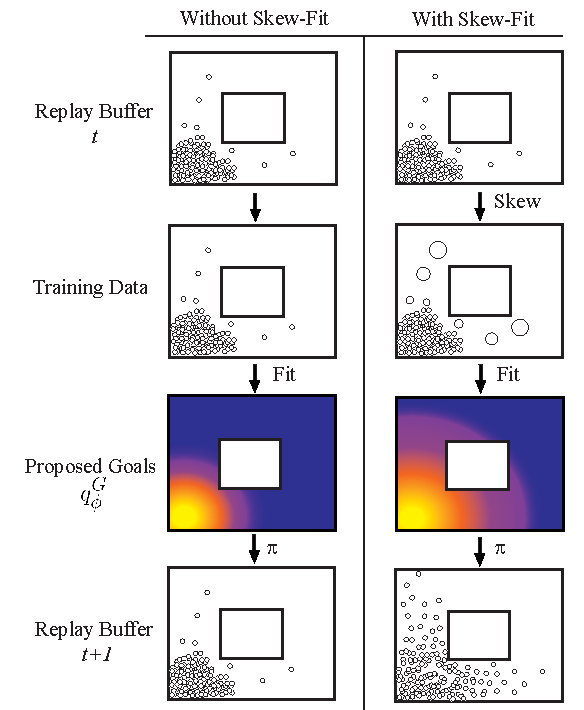
\includegraphics[width=\linewidth]{skewfit/figures/skewfitfigure_vertical_q_phi_g.pdf}
    \fcaption{Our method, \METHOD, samples goals for goal-conditioned RL.
    We sample states from our replay buffer, and give more weight to rare states.
    We then train a generative model $\pg_{t+1}$ with the weighted samples.
    By sampling new states with goals proposed from this new generative model, we obtain a higher entropy state distribution in the next iteration.}
    \label{fig:main-fig}
\end{figure}

The intuition behind our method is simple: rather than fitting a generative model to these samples $\st_n$, we \textit{skew} the samples so that rarely visited states are given more weight.
See \Figref{fig:main-fig} for a visualization of this process.
How should we skew the samples if we want to maximize the entropy of $\pgtt$?
If we had access to the density of each state, $\pet(\St)$, then we could simply weight each state by $1/\pet(\St)$.
We could then perform maximum likelihood estimation (MLE) for the uniform distribution by using the following importance sampling (IS) loss to train $\pgparamtt$:
\begin{align}
\Loss(\pgparam)\nonumber
    &= \E_{\St \sim \U} \left[ \log \pg(\St)\right]
\\\nonumber
    &= \E_{\St \sim \pet}\left[ \frac{\U(\St)}{\pet(\St)} \log \pg(\St)\right]
\\\nonumber
    &\propto \E_{\St \sim \pet}\left[ \frac{1}{\pet(\St)}\log \pg(\St)\right]
\nonumber
\end{align}
where we use the fact that the uniform distribution $\U(\St)$ has constant density for all states in $\Imgs$.
However, computing this density $\pet(\St)$ requires marginalizing out the MDP dynamics, which requires an accurate model of both the dynamics and the goal-conditioned policy.

We avoid needing to model the entire MDP process by approximating $\pet(\St)$ with our previous learned generative model: \mbox{$\pstatet(\St) \approx \pgt(\St)$}.
We therefore weight each state by the following weight function
\begin{align}\label{eq:weight-defn}
    \wt(\SF) \triangleq \pgt(\SF)^\alpha, \quad \alpha < 0.
\end{align}
where $\alpha$ is a hyperparameter that controls how heavily we weight each state.
If our approximation $\pgt$ is exact, we can choose $\alpha = -1$ and recover the exact IS procedure described above.
If $\alpha = 0$, then this skew step has no effect.
By choosing intermediate values of $\alpha$, we trade off the reliability of our estimate $\pgt(\St)$ with the speed at which we want to increase the goal distribution entropy.

\paragraph{Variance Reduction}
As described, this procedure relies on IS, which can have high variance, particularly if $\pgt(\St) \approx 0$.
We therefore choose a class of generative models where the probabilities are prevented from collapsing to zero, as we will describe in \autoref{sec:train-policy} where we provide generative model details.
To further reduce the variance, we train $\pgtt$ with sampling importance resampling (SIR)~\citep{rubin1988using} rather than IS.
Rather than sampling from $\pet$ and weighting the update from each sample by $\wt$, SIR explicitly defines a skewed empirical distribution as
\begin{align}\label{eq:pskew-defn}
    \pskewedt(\st) \triangleq \frac{1}{Z_\alpha} \wt(\st) \delta(\st \in \{\st_n\}_{n=1}^{N})
    \\\nonumber
    Z_\alpha = \sum_{n=1}^N \wt(\st_n),\ \st_n \overset{\text{iid}}{\sim} \pstatet,
\end{align}
where $\delta$ is the indicator function and $Z_\alpha$ is the normalizing coefficient.
We note that computing $Z_\alpha$ adds little computational overhead, since all of the weights already need to be computed.
We then fit the generative model at the next iteration $\pgtt$ to $\pskewedt$ using standard MLE.
We found that using SIR resulted in significantly lower variance than IS.
See \autoref{sec:analysis-variance} for this comparision.

\paragraph{Goal Sampling Alternative}
Because $\pgtt \approx \pskewedt$, at iteration $t+1$, one can sample goals from either $\pgtt$ or $\pskewedt$.
Sampling goals from $\pskewedt$ may be preferred if sampling from the learned generative model $\pgtt$ is computationally or otherwise challenging.
In either case, one still needs to train the generative model $\pgt$ to create $\pskewedt$.
In our experiments, we found that both methods perform well.

\paragraph{Summary}
Overall, \METHOD collects states from the environment and resamples each state in proportion to \autoref{eq:weight-defn} so that low-density states are resampled more often.
\METHOD is shown in \Figref{fig:main-fig} and summarized in Algorithm \ref{alg:method}.
We now discuss conditions under which \METHOD converges to the uniform distribution.

\vspace{0.1in}
\begin{algorithm}
   	\fcaption{\METHOD}
   	\label{alg:method}
   	\begin{algorithmic}[1]
   	\FOR{Iteration $t=1, 2, ...$}
        \STATE Collect $N$ states $\{\st_n\}_{n=1}^N$ by sampling goals from $\pgt$ (or $\pskewed_{t-1}$) and running goal-conditioned policy.
        \STATE Construct skewed distribution $\pskewedt$ (\Eqref{eq:weight-defn} and \Eqref{eq:pskew-defn}).
        \STATE Fit $\pgtt$ to skewed distribution $\pskewedt$ using MLE.
   	\ENDFOR
   	\end{algorithmic}
\end{algorithm}

\subsection{\METHOD Analysis}\label{sec:analysis}
This section provides conditions under which $\pgt$ converges in the limit to the uniform distribution over the state space $\Imgs$.
We consider the case where $N \rightarrow \infty$, which allows us to study the limit behavior of the goal distribution $\pskewedt$.
Our most general result is stated as follows:
\begin{lemma}\label{lemma:general-convergence}
Let $\Imgs$ be a compact set.
Define the set of distributions $\gQ = \{p : \support(p) \subseteq \Imgs\}$.
Let $\gF: \gQ \mapsto \gQ$ be continuous with respect to the pseudometric \mbox{$\dent(p, q) \triangleq |\gH(p) - \gH(q)|$} and $\gH(\gF(p)) \geq \gH(p)$ with equality if and only if $p$ is the uniform probability distribution on $\Imgs$, denoted as $\U$.
Define the sequence of distributions $P = (p_1, p_2, \dots)$ by starting with any $p_1 \in \gQ$ and recursively defining $p_{t+1} = \gF(p_t)$.
The sequence $P$ converges to $\U$ with respect to $\dent$. In other words, \mbox{$\lim_{t \rightarrow 0} |\gH(p_t) - \gH(\U)| \rightarrow 0$}.
\end{lemma}
\begin{proof}
See Appendix Section \ref{sec:general-proof}.
\end{proof}

We will apply Lemma \ref{lemma:general-convergence} to be the map from $\pskewedt$ to $\pskewedtt$ to show that $\pskewedt$ converges to $\U$.
If we assume that the goal-conditioned policy and generative model learning procedure are well behaved
(i.e., the maps from $\pgt$ to $\pet$ and from $\pskewedt$ to $\pgtt$ are continuous),
then to apply Lemma~\ref{lemma:general-convergence}, we only need to show that \mbox{$\gH(\pskewedt) \geq \gH(\pet)$} with equality if and only if \mbox{$\pet = \U$}.
For the simple case when \mbox{$\pgt = \pet$} identically at each iteration, we prove the convergence of \METHOD true for any value of $\alpha \in [-1, 0)$ in \autoref{sec:simple-case-proof}.
However, in practice, $\pgt$ only approximates $\pet$. To address this more realistic situation, we prove the following result:
\begin{lemma}\label{lemma:pos-cov-negative-grad}
Given two distribution $\pet$ and $\pgt$ where $\pet \ll \pgt$
\footnote{
$p \ll q$ means that $p$ is absolutely continuous with respect to $q$, i.e. $p(\st) = 0 \implies q(\st) = 0$.
}
and
\begin{align}\label{eq:pos-cov}
  \Cov_{\St \sim \pet}\left[\log \pet(\St), \log \pgt(\St)\right] > 0,
\end{align}
define the $\pskewedt$ as in \Eqref{eq:pskew-defn} and take $N \rightarrow \infty$.
Let $\gH_\alpha(\alpha)$ be the entropy of $\pskewedt$ for a fixed $\alpha$.
Then there exists a constant $a < 0$ such that for all $\alpha \in [a, 0)$,
\begin{align*}
    \gH(\pskewedt) =  \gH_\alpha(\alpha) > \gH(\pet).
\end{align*}
\end{lemma}
\begin{proof}
See Appendix Section \ref{sec:covariance-proof}.
\end{proof}
This lemma tells us that our generative model $\pgt$ does not need to exactly fit the sampled states.
Rather, we merely need the log densities of $\pgt$ and $\pet$ to be correlated, which we expect to happen frequently with an accurate goal-conditioned policy, since $\pet$ is the set of states seen when trying to reach goals from $\pgt$.
In this case, if we choose negative values of $\alpha$ that are small enough, then the entropy of $\pskewedt$ will be higher than that of $\pet$.
Empirically, we found that $\alpha$ values as low as $\alpha=-1$ performed well.

In summary, $\pskewedt$ converges to $\U$ under certain assumptions.
Since we train each generative model $\pgtt$ by fitting it to $\pskewedt$ with MLE, $\pgt$ will also converge to $\U$.


\section{Training Goal-Conditioned Policies with \METHOD}
\label{sec:train-policy}
Thus far, we have presented \METHOD assuming that we have access to a goal-reaching policy, allowing us to separately analyze how we can maximize $\HG$.
However, in practice we do not have access to such a policy, and this section discusses how we concurrently train a goal-reaching policy.

Maximizing $I(\SF; \G)$ can be done by simultaneously performing \METHOD and training a goal-conditioned policy to minimize $\HGS$, or, equivalently, maximize $-\HGS$.
Maximizing $-\HGS$ requires computing the density $\log p(\G \mid \SF)$, which may be difficult to compute without strong modeling assumptions.
However, for any distribution $q$, the following lower bound on $-\HGS$:
\begin{align}\nonumber
-\HGS
    &= \E_{(\G, \SF) \sim q}\left[
        \log q(\G \mid \SF)
    \right]
+ \kld{p}{q}
\\\nonumber
&
    \geq \E_{(\G, \SF) \sim q}\left[
        \log q(\G \mid \SF)
    \right],
\end{align}
where $\KL$ denotes Kullback–Leibler divergence as discussed by \citet{barber2004information}.
Thus, to minimize $\HGS$, we train a policy to maximize the reward
\begin{align}\nonumber
    r(\SF, \G) = \log q(\G \mid \SF).
\end{align}

The RL algorithm we use is reinforcement learning with imagined goals (RIG)~\citep{nair2018rig}, though in principle any goal-conditioned method could be used.
RIG is an efficient off-policy goal-conditioned method that solves vision-based RL problems in a learned latent space.
In particular, RIG fits a $\beta$-VAE~\citep{higgins2016beta} and uses it to encode observations and goals into a latent space, which it uses as the state representation.
RIG also uses the $\beta$-VAE to compute rewards, $\log q(\G \mid \SF)$.
Unlike RIG, we use the goal distribution from \METHOD to sample goals for exploration and for relabeling goals during training~\citep{andrychowicz2017her}.
Since RIG already trains a generative model over states, we reuse this $\beta$-VAE for the generative model $\pg$ of \METHOD.
To make the most use of the data, we train $\pg$ on all visited state rather than only the terminal states, which we found to work well in practice.
To prevent the estimated state likelihoods from collapsing to zero, we model the posterior of the $\beta$-VAE as a multivariate Gaussian distribution with a fixed variance and only learn the mean.
We summarize RIG and provide details for how we combine \METHOD and RIG in \autoref{sec:rig-and-full-method} and describe how we estimate the likelihoods given the $\beta$-VAE in \autoref{sec:likelihood-estimation-vae}.


\section{Related Work}\label{sec:related_work}
Many prior methods in the goal-conditioned reinforcement learning literature focus on training goal-conditioned policies and assume that a goal distribution is available to sample from during exploration~\citep{kaelbling1993goals,schaul2015uva,andrychowicz2017her,pong2018tdm}, or use a heuristic to design a non-parametric~\citep{colas2018gep,wardefarley2018discern,florensa2018selfsupervised} or parametric~\citep{pere2018unsupervised,nair2018rig} goal distribution based on previously visited states.
These methods are largely complementary to our work:
rather than proposing a better method for training goal-reaching policies, we propose a principled method for maximizing the entropy of a goal sampling distribution, $\gH(\G)$, such that these policies cover a wide range of states.

Our method learns without any task rewards, directly acquiring a policy that can be reused to reach user-specified goals.
This stands in contrast to exploration methods that modify the reward based on state visitation frequency~\citep{bellemare2016unifying,ostrovski2017count,tang2017hashtag,chentanez2005intrinsically,lopes2012exploration,stadie2016exploration,pathak2017curiosity,burda2018exploration,burda2018large,mohamed2015variational,tang2017hashtag,fu2017ex2}.
While these methods can also be used without a task reward, they provide no mechanism for distilling the knowledge gained from visiting diverse states into flexible policies that can be applied to accomplish new goals at test-time: their policies visit novel states, and they quickly forget about them as other states become more novel.
Similarly, methods that provably maximize state entropy without using goal-directed exploration~\citep{hazan2019provably} or methods that define new rewards to capture measures of intrinsic motivation~\citep{mohamed2015variational} and reachability~\citep{savinov2018episodic} do not produce reusable policies.

Other prior methods extract reusable skills in the form of latent-variable-conditioned policies, where
latent variables are interpreted as options~\citep{sutton1999between} or abstract skills~\citep{hausman2018skillembedding,gupta2018structuredexploration,eysenbach2018diayn,gupta2018unsupervised,florensa2017stochastic}.
The resulting skills are diverse, but have no grounded interpretation, while \METHOD policies can be used immediately after unsupervised training to reach diverse user-specified goals.

Some prior methods propose to choose goals based on heuristics such as learning progress~\citep{baranes2012, veeriah2018many, colas2018curious}, how off-policy the goal is~\citep{nachum2018hiro}, level of difficulty~\citep{held2018goalgan}, or likelihood ranking~\citep{zhao2019rankweight}.
In contrast, our approach provides a principled framework for optimizing a concrete and well-motivated exploration objective, can provably maximize this objective under regularity assumptions, and empirically outperforms many of these prior work (see \autoref{sec:experiments}).

\section{Experiments}\label{sec:experiments}
Our experiments study the following questions:
\textbf{(1)} Does \METHOD empirically result in a goal distribution with increasing entropy?
\textbf{(2)} Does \METHOD improve exploration for goal-conditioned RL?
\textbf{(3)} How does \METHOD compare to prior work on choosing goals for vision-based, goal-conditioned RL?
\textbf{(4)} Can \METHOD be applied to a real-world, vision-based robot task?

\begin{figure}[t]
    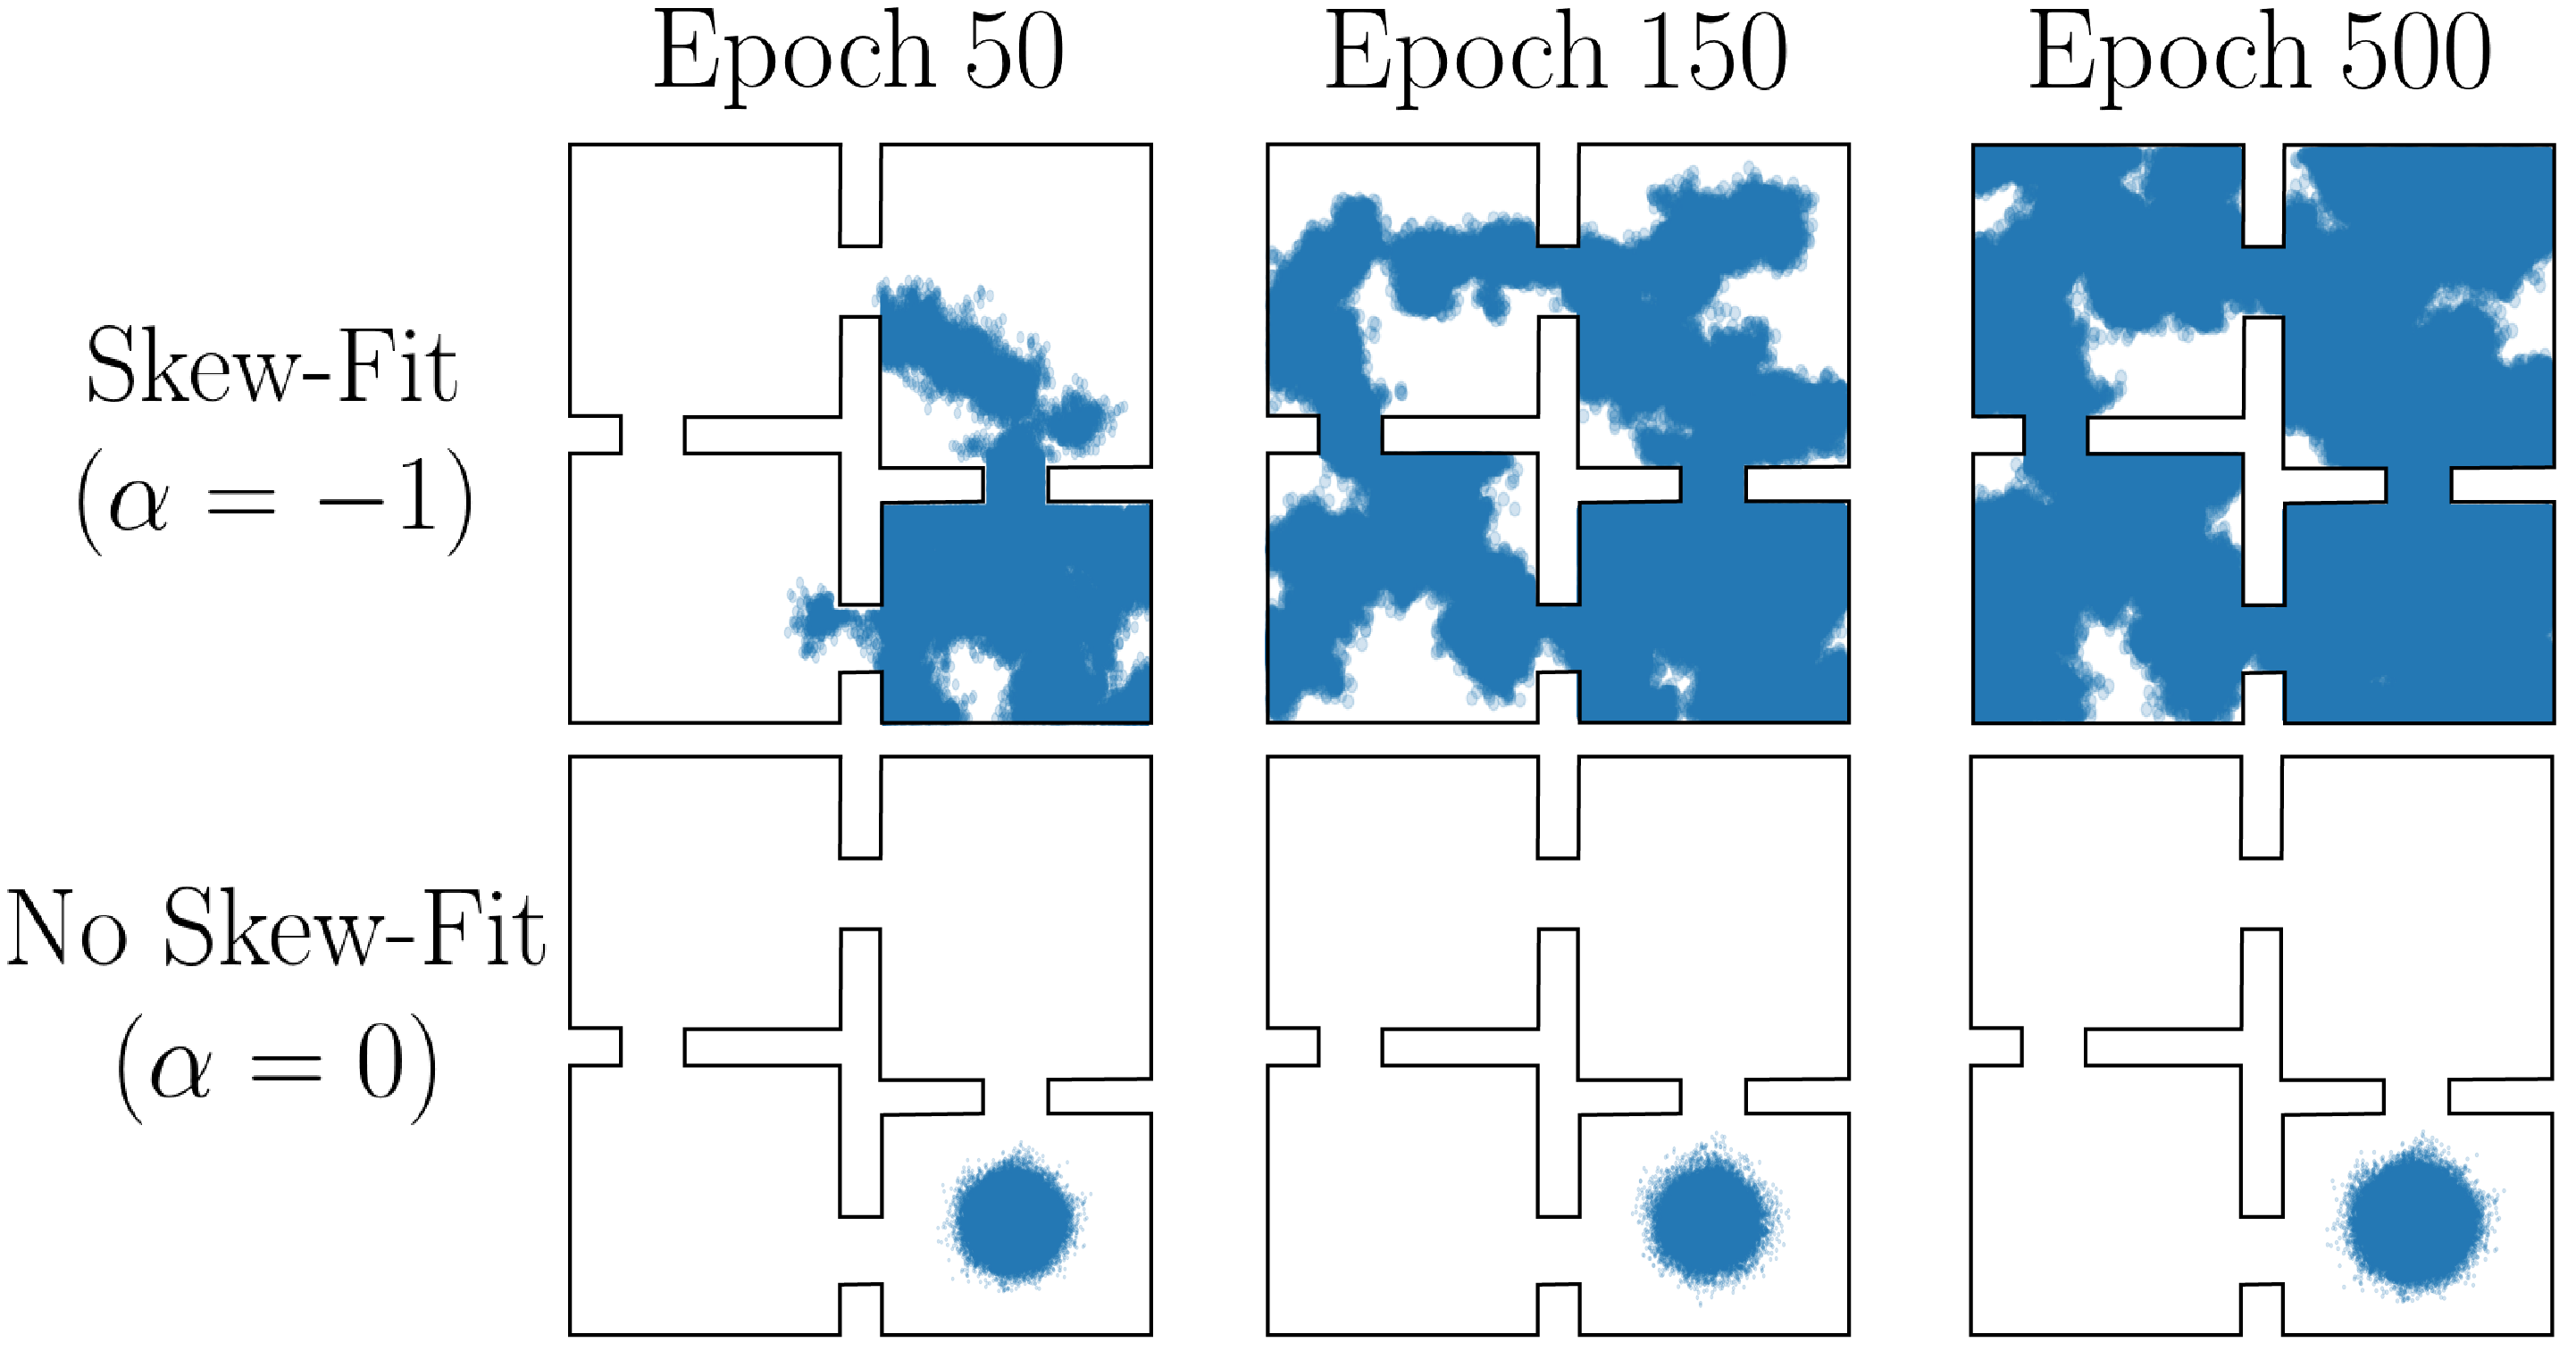
\includegraphics[width=.49\linewidth ]{skewfit/figures/entropy_figure-01.png}
    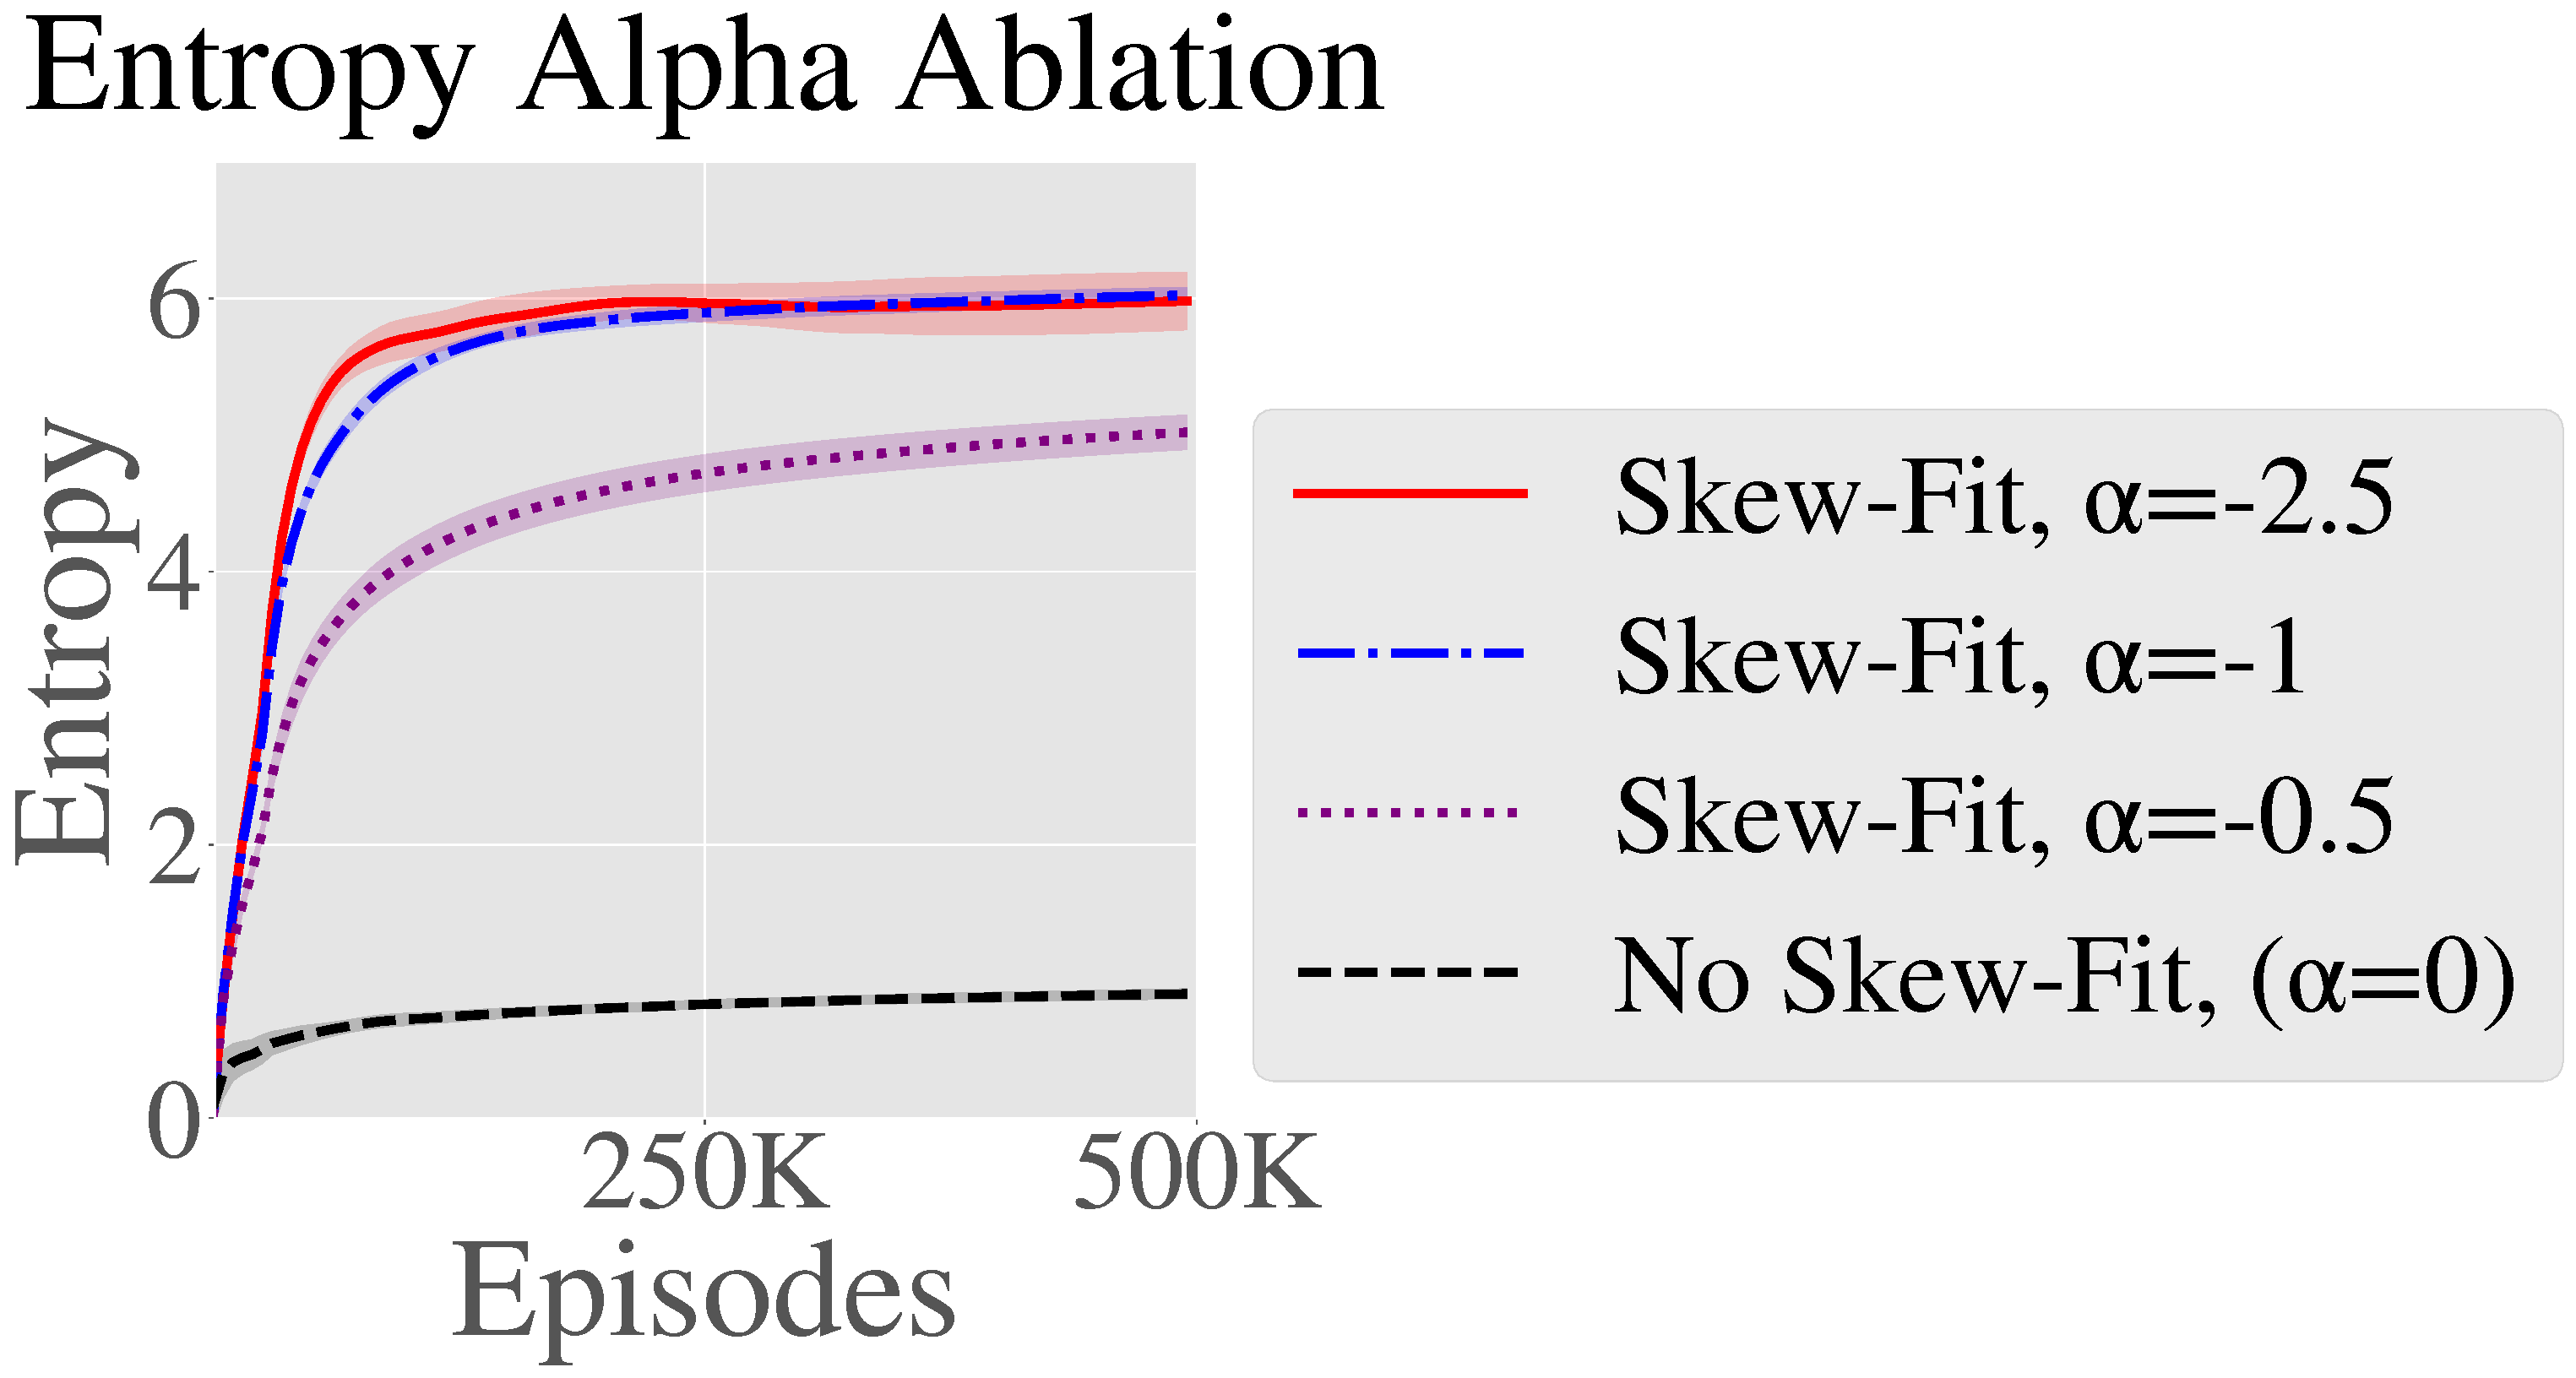
\includegraphics[width=.49\linewidth ]{skewfit/figures/plots/four_rooms_entropy}
    \fcaption{
    Illustrative example of \METHOD on a 2D navigation task. (Left) Visited state plot for \METHOD with $\alpha = -1$ and uniform sampling, which corresponds to $\alpha = 0$. (Right) The entropy of the goal distribution per iteration, mean and standard deviation for 9 seeds. Entropy is calculated via discretization onto an 11x11 grid. \METHOD steadily increases the state entropy, reaching full coverage over the state space.
    }
    \label{fig:2d-sl}
\end{figure}

\paragraph{Does \METHOD Maximize Entropy?}
To see the effects of \METHOD on goal distribution entropy in isolation of learning a goal-reaching policy, we study an idealized example where the policy is a near-perfect goal-reaching policy.
The environment consists of four rooms~\citep{sutton1999between}.
At the beginning of an episode, the agent begins in the bottom-right room and samples a goal from the goal distribution $\pgt$.
To simulate stochasticity of the policy and environment, we add a Gaussian noise with standard deviation of $0.06$ units to this goal, where the entire environment is $11 \times 11$ units.
The policy reaches the state that is closest to this noisy goal and inside the rooms, giving us a state sample $\st_n$ for training $\pgt$.
Due to the relatively small noise, the agent cannot rely on this stochasticity to explore the different rooms and must instead learn to set goals that are progressively farther and farther from the initial state.
We compare multiple values of $\alpha$, where $\alpha=0$ corresponds to not using \METHOD.
The $\beta$-VAE hyperparameters used to train $\pgt$ are given in \autoref{sec:2d-details}.
As seen in \Figref{fig:2d-sl}, sampling uniformly from previous experience ($\alpha = 0$) to set goals results in a policy that primarily sets goal near the initial state distribution.
In contrast, \METHOD results in quickly learning a high entropy, near-uniform distribution over the state space.

\begin{figure}[t]
    \centering
    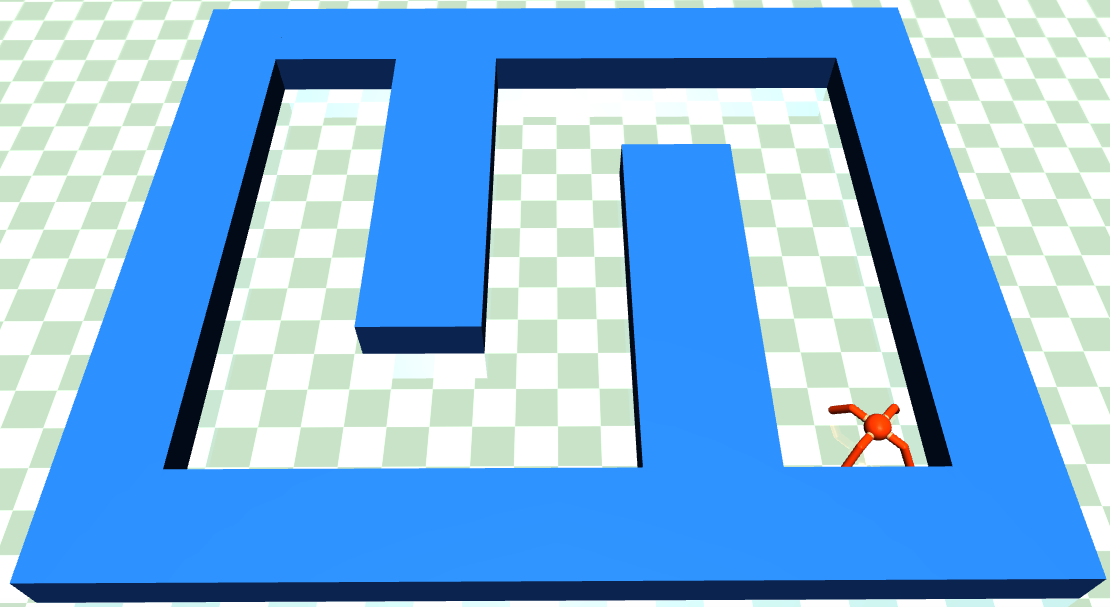
\includegraphics[width=0.32\linewidth]{skewfit/figures/ant_env_updated.png}
    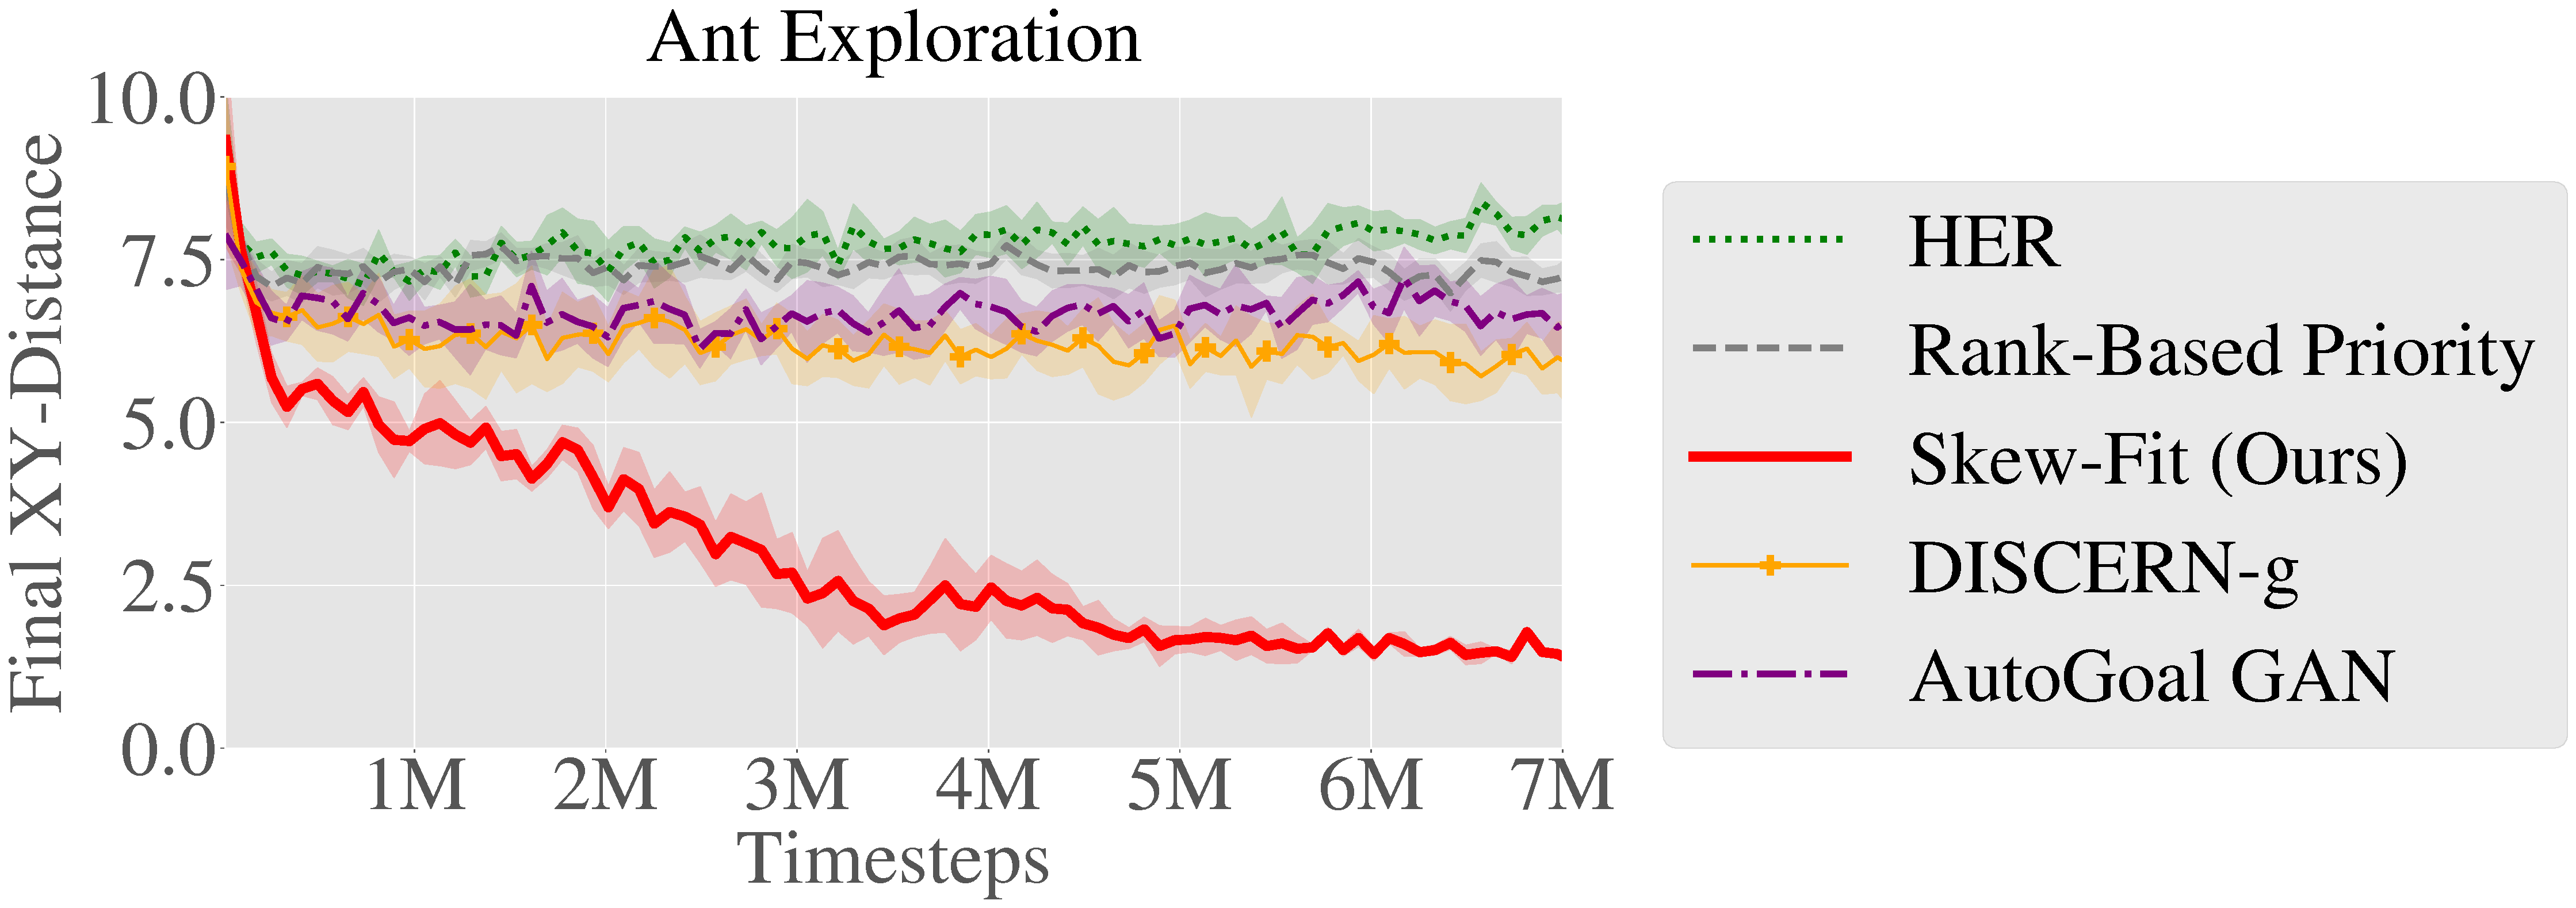
\includegraphics[width=0.65\linewidth]{skewfit/figures/plots/ant.pdf}
    \fcaption{
    (Left) Ant navigation environment.
    (Right) Evaluation on reaching target XY position.
    We show the mean and standard deviation of 6 seeds.
    \METHOD significantly outperforms prior methods on this exploration task.
    }
    \label{fig:antmaze}
\end{figure}

\paragraph{Exploration with \METHOD}
We next evaluate \METHOD while concurrently learning a goal-conditioned policy on a task with state inputs, which enables us study exploration performance independently of the challenges with image observations.
We evaluate on a task that requires training a simulated quadruped ``ant'' robot to navigate to different XY positions in a labyrinth,
as shown in \Figref{fig:antmaze}.
The reward is the negative distance to the goal XY-position, and additional environment details are provided in \autoref{sec:environment-details}.
This task presents a challenge for goal-directed exploration:
the set of valid goals is unknown due to the walls, and
random actions do not result in exploring locations far from the start.
Thus, \METHOD must set goals that meaningfully explore the space while simultaneously learning to reach those goals.

We use this domain to compare \METHOD to a number of existing goal-sampling methods.
We compare to the relabeling scheme described in the hindsight experience replay (labeled \textbf{HER}).
We compare to curiosity-driven prioritization (\textbf{Ranked-Based Priority})~\citep{zhao2019maximum}, a variant of HER that samples goals for relabeling based on their ranked likelihoods.
\citet{held2018goalgan} samples goals from a GAN based on the difficulty of reaching the goal.
We compare against this method by replacing $\pg$ with the GAN and label it \textbf{AutoGoal GAN}.
We also compare to the non-parametric goal proposal mechanism proposed by \cite{wardefarley2018discern}, which we label \textbf{DISCERN-g}.
Lastly, to demonstrate the difficulty of the exploration challenge in these domains, we compare to \textbf{\#-Exploration}~\citep{tang2017hashtag}, an exploration method that assigns bonus rewards based on the novelty of new states.
We train the goal-conditioned policy for each method using soft actor critic (SAC)~\citep{haarnoja2018sacapp}.
Implementation details of SAC and the prior works are given in  \autoref{sec:prior-work-implementation}.

We see in \Figref{fig:antmaze} that \METHOD is the only method that makes significant progress on this challenging labyrinth locomotion task.
The prior methods on goal-sampling primarily set goals close to the start location, while the extrinsic exploration reward in \#-Exploration dominated the goal-reaching reward.
These results demonstrate that \METHOD accelerates exploration by setting diverse goals in tasks with unknown goal spaces.


\paragraph{Vision-Based Continuous Control Tasks}
\begin{figure}[t]
    \centering
    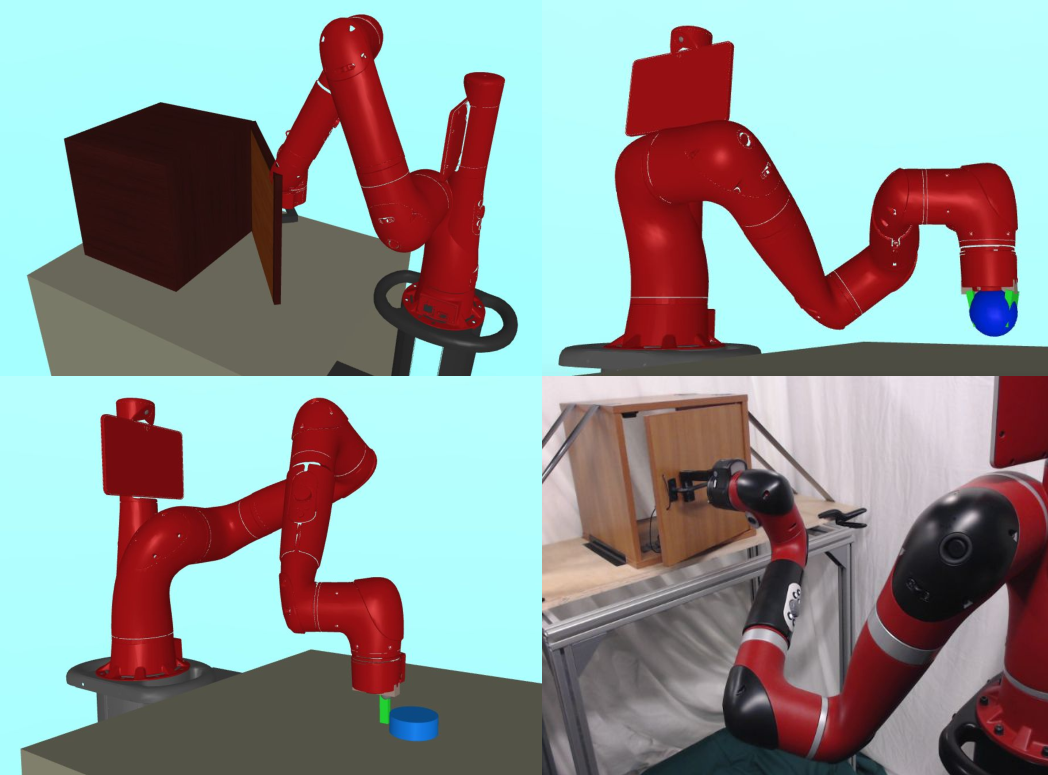
\includegraphics[width=0.8\linewidth]{skewfit/figures/env_display.pdf}
    \fcaption{We evaluate on these continuous control tasks, from left to right:
    \textit{Visual Door}, a door opening task;
    \textit{Visual Pickup}, a picking task;
    \textit{Visual Pusher}, a pushing task;
    and \textit{Real World Visual Door}, a real world door opening task. All tasks are solved from images and without any task-specific reward. See Appendix \ref{sec:environment-details} for details.}
    \label{fig:env-pics}
\end{figure}

We now evaluate \METHOD on a variety of image-based continuous control tasks, where the policy must control a robot arm using only image observations, there is no state-based or task-specific reward, and \METHOD must directly set image goals.
We test our method on three different image-based simulated continuous control tasks released by the authors of RIG~\citep{nair2018rig}: \textit{Visual Door}, \textit{Visual Pusher}, and \textit{Visual Pickup}.
These environments contain a robot that can open a door, push a puck, and lift up a ball to different configurations, respectively.
To our knowledge, these are the only goal-conditioned, vision-based continuous control environments that are publicly available and experimentally evaluated in prior work, making them a good point of comparison.
See \autoref{fig:env-pics} for visuals and \autoref{sec:implementation-details} for environment details.
The policies are trained in a completely unsupervised manner, without access to any prior information about the image-space or any pre-defined goal-sampling distribution.
To evaluate their performance, we sample goal images from a uniform distribution over valid states and report the agent's final distance to the corresponding simulator states (e.g., distance of the object to the target object location), but the agent never has access to this true uniform distribution nor the ground-truth state information during training.
While this evaluation method is only practical in simulation, it provides us with a quantitative measure of a policy's ability to reach a broad coverage of goals in a vision-based setting.

We compare \METHOD to a number of existing methods on this domain.
First, we compare to the methods described in the previous experiment (HER, Rank-Based Priority, \#-Exploration, Autogoal GAN, and \mbox{DISCERN-g}).
These methods that we compare to were developed in non-vision, state-based environments.
To ensure a fair comparison across methods, we combine these prior methods with a policy trained using RIG.
We additionally compare to \citet{hazan2019provably}, an exploration method that assigns bonus rewards based on the likelihood of a state (labeled \textbf{Hazan et al.}).
Next, we compare to \textbf{RIG} without \METHOD.
Lastly, we compare to \textbf{DISCERN}~\citep{wardefarley2018discern}, a vision-based method which uses a non-parametric clustering approach to sample goals and an image discriminator to compute rewards.

\begin{figure}
    \centering
     \begin{subfigure}[t]{.49\linewidth}
    \centering
        % 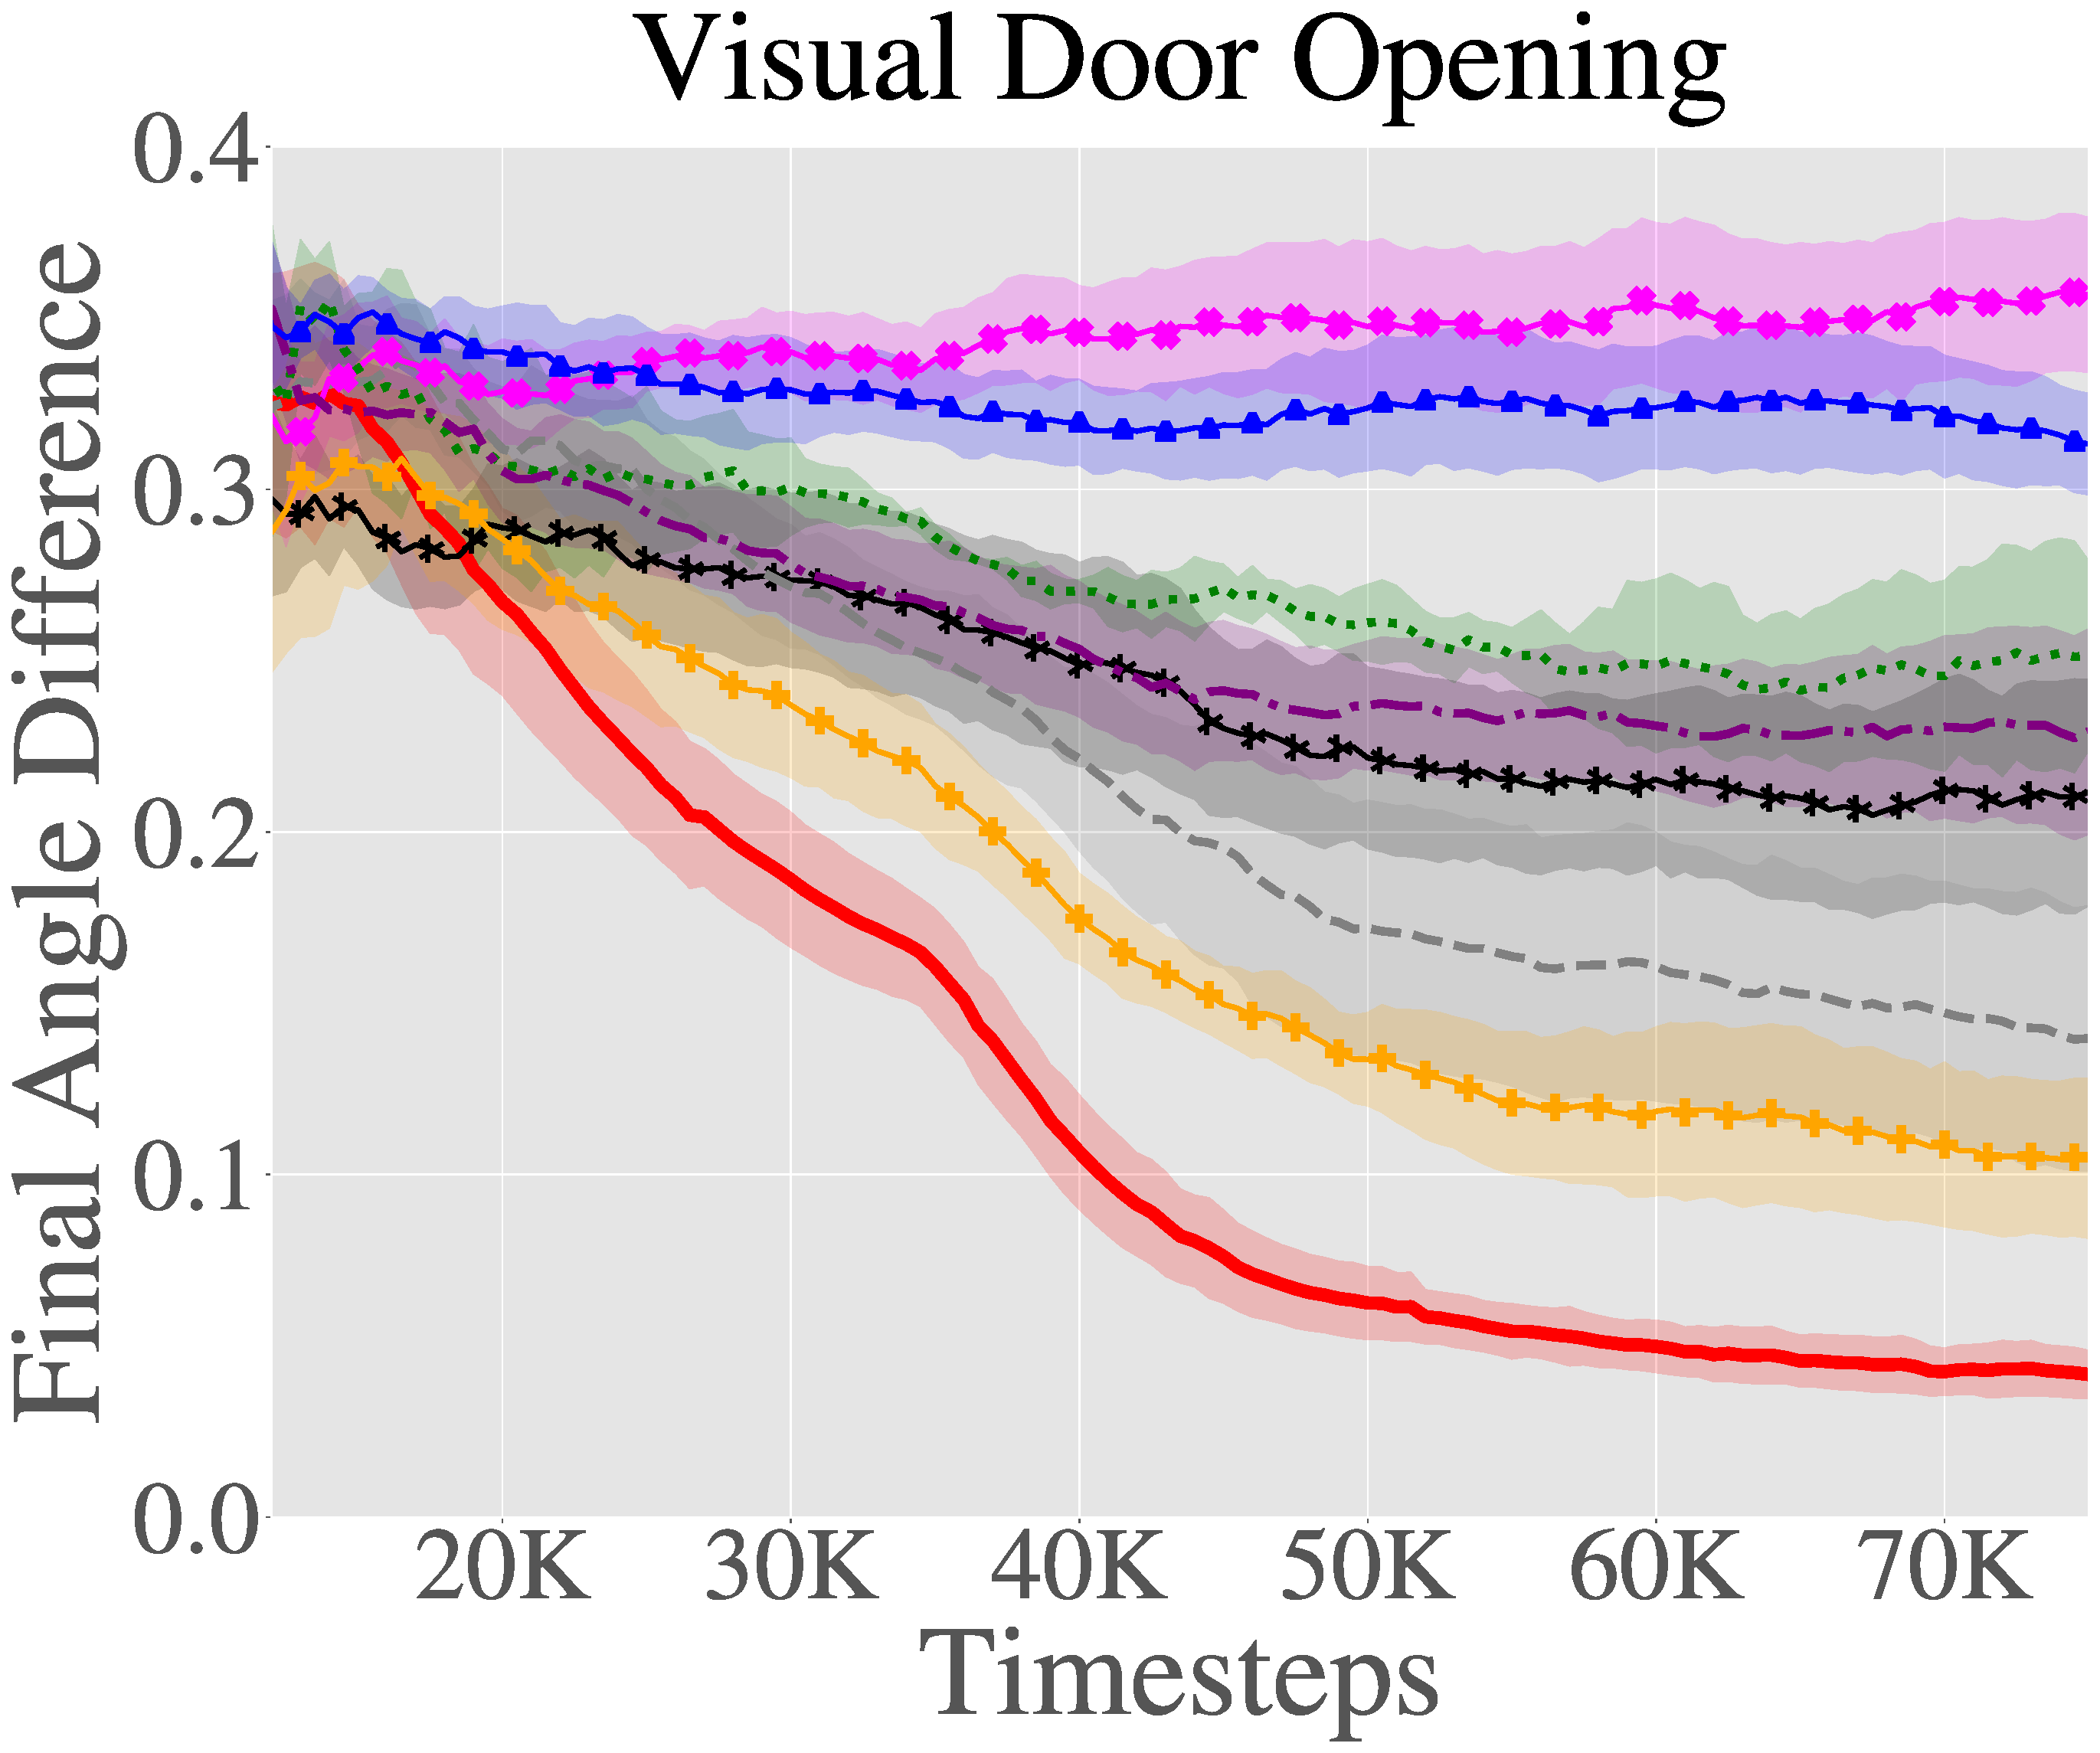
\includegraphics[width=\linewidth]{skewfit/figures/plots/main_sim_fig/door_big.pdf}
          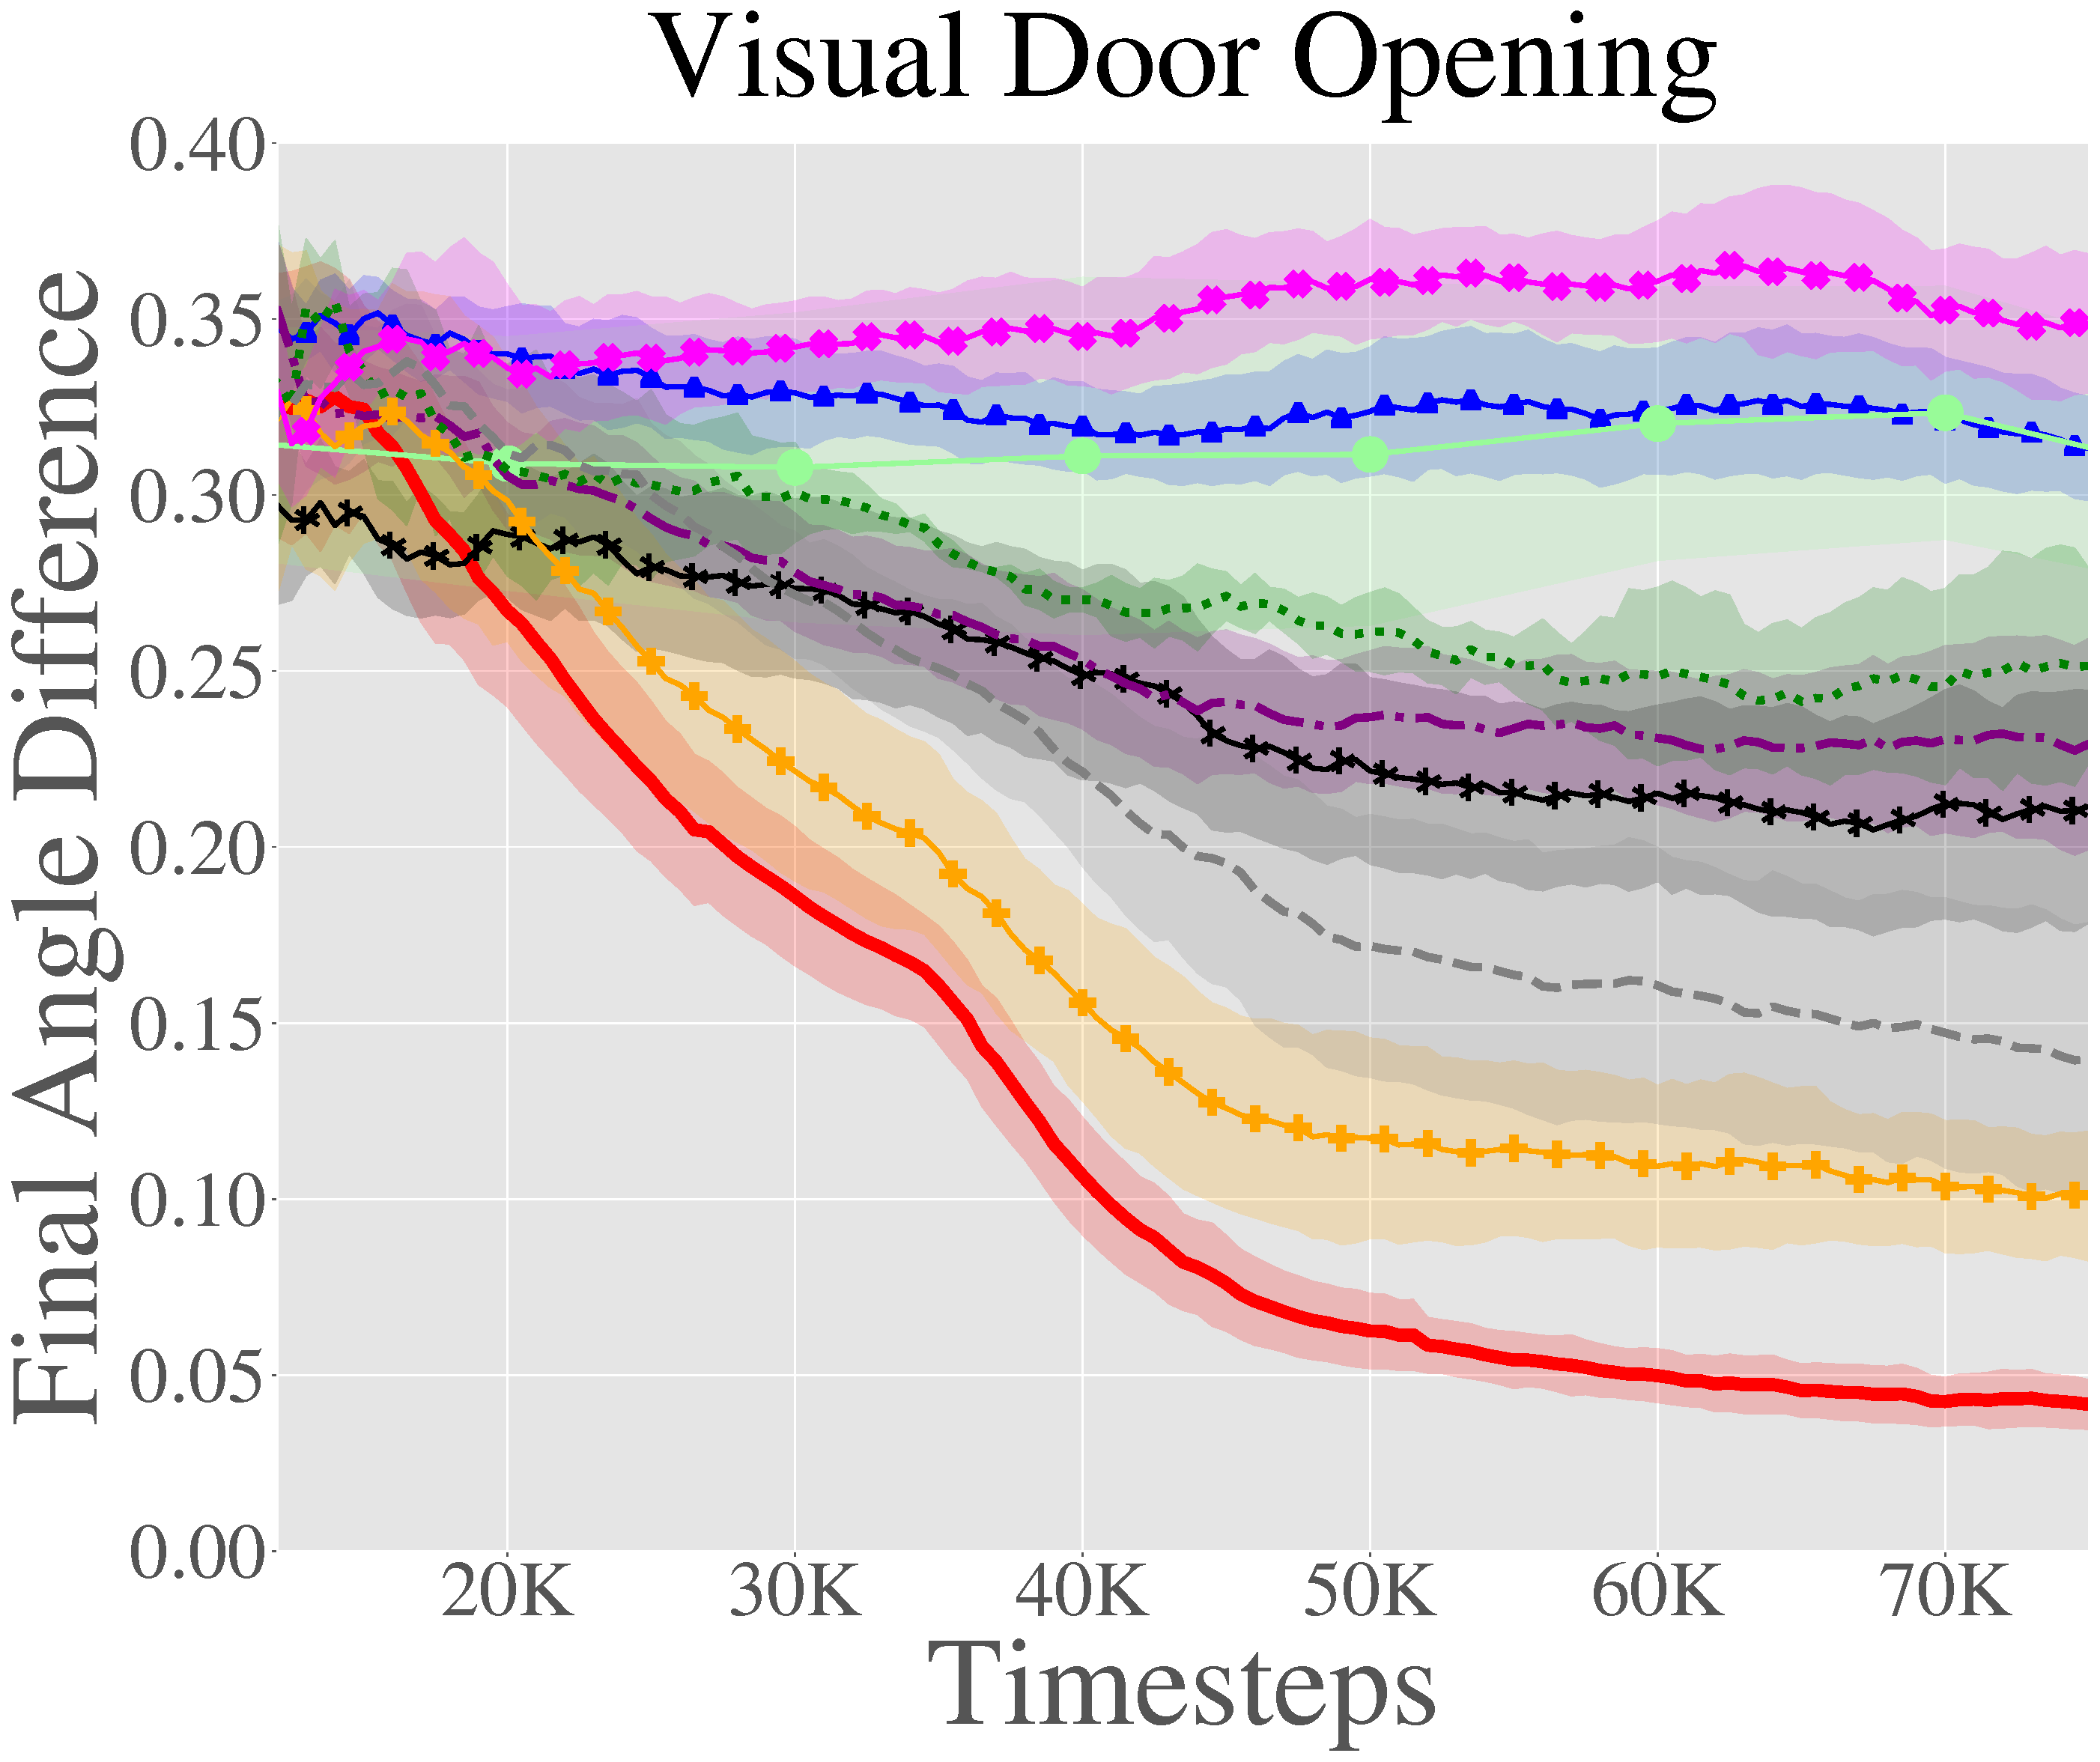
\includegraphics[width=\linewidth]{skewfit/figures/plots/main_sawyer_fig_with_hazan/door.pdf}
  \end{subfigure}
  \hfill
  \begin{subfigure}[t]{.49\linewidth}
    \centering
        % 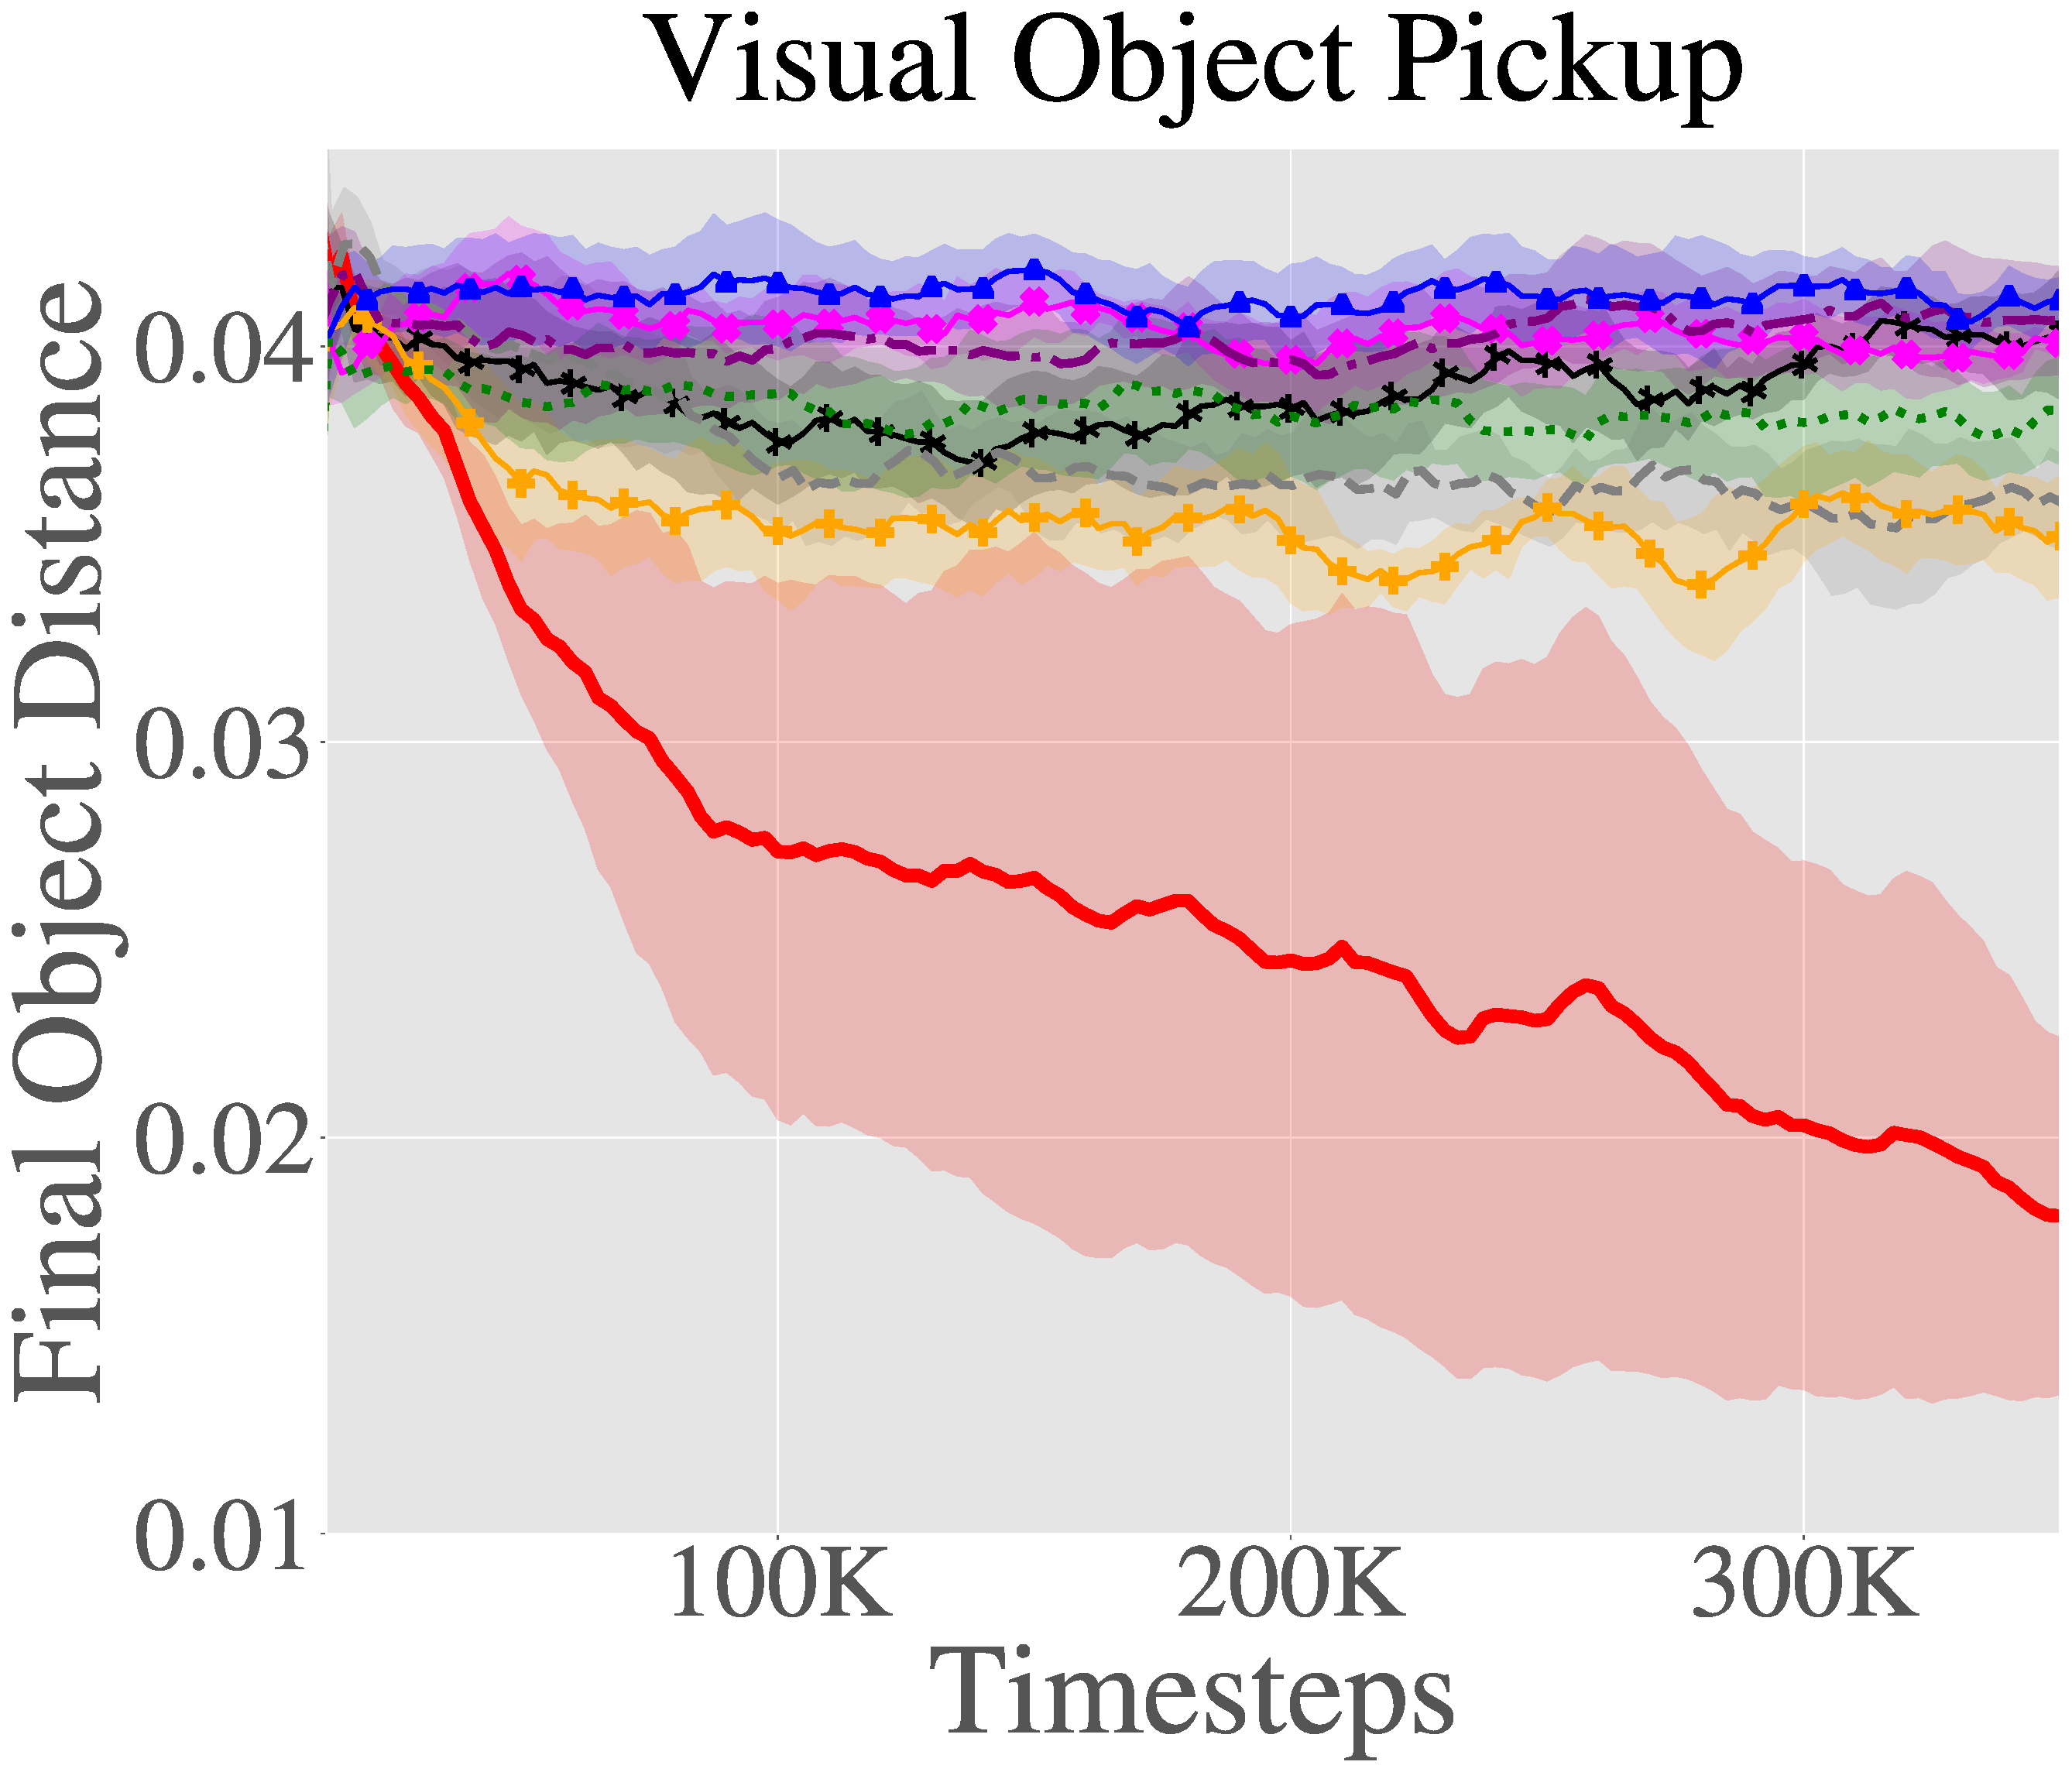
\includegraphics[width=\linewidth]{skewfit/figures/plots/main_sim_fig/pickup_big.pdf}
          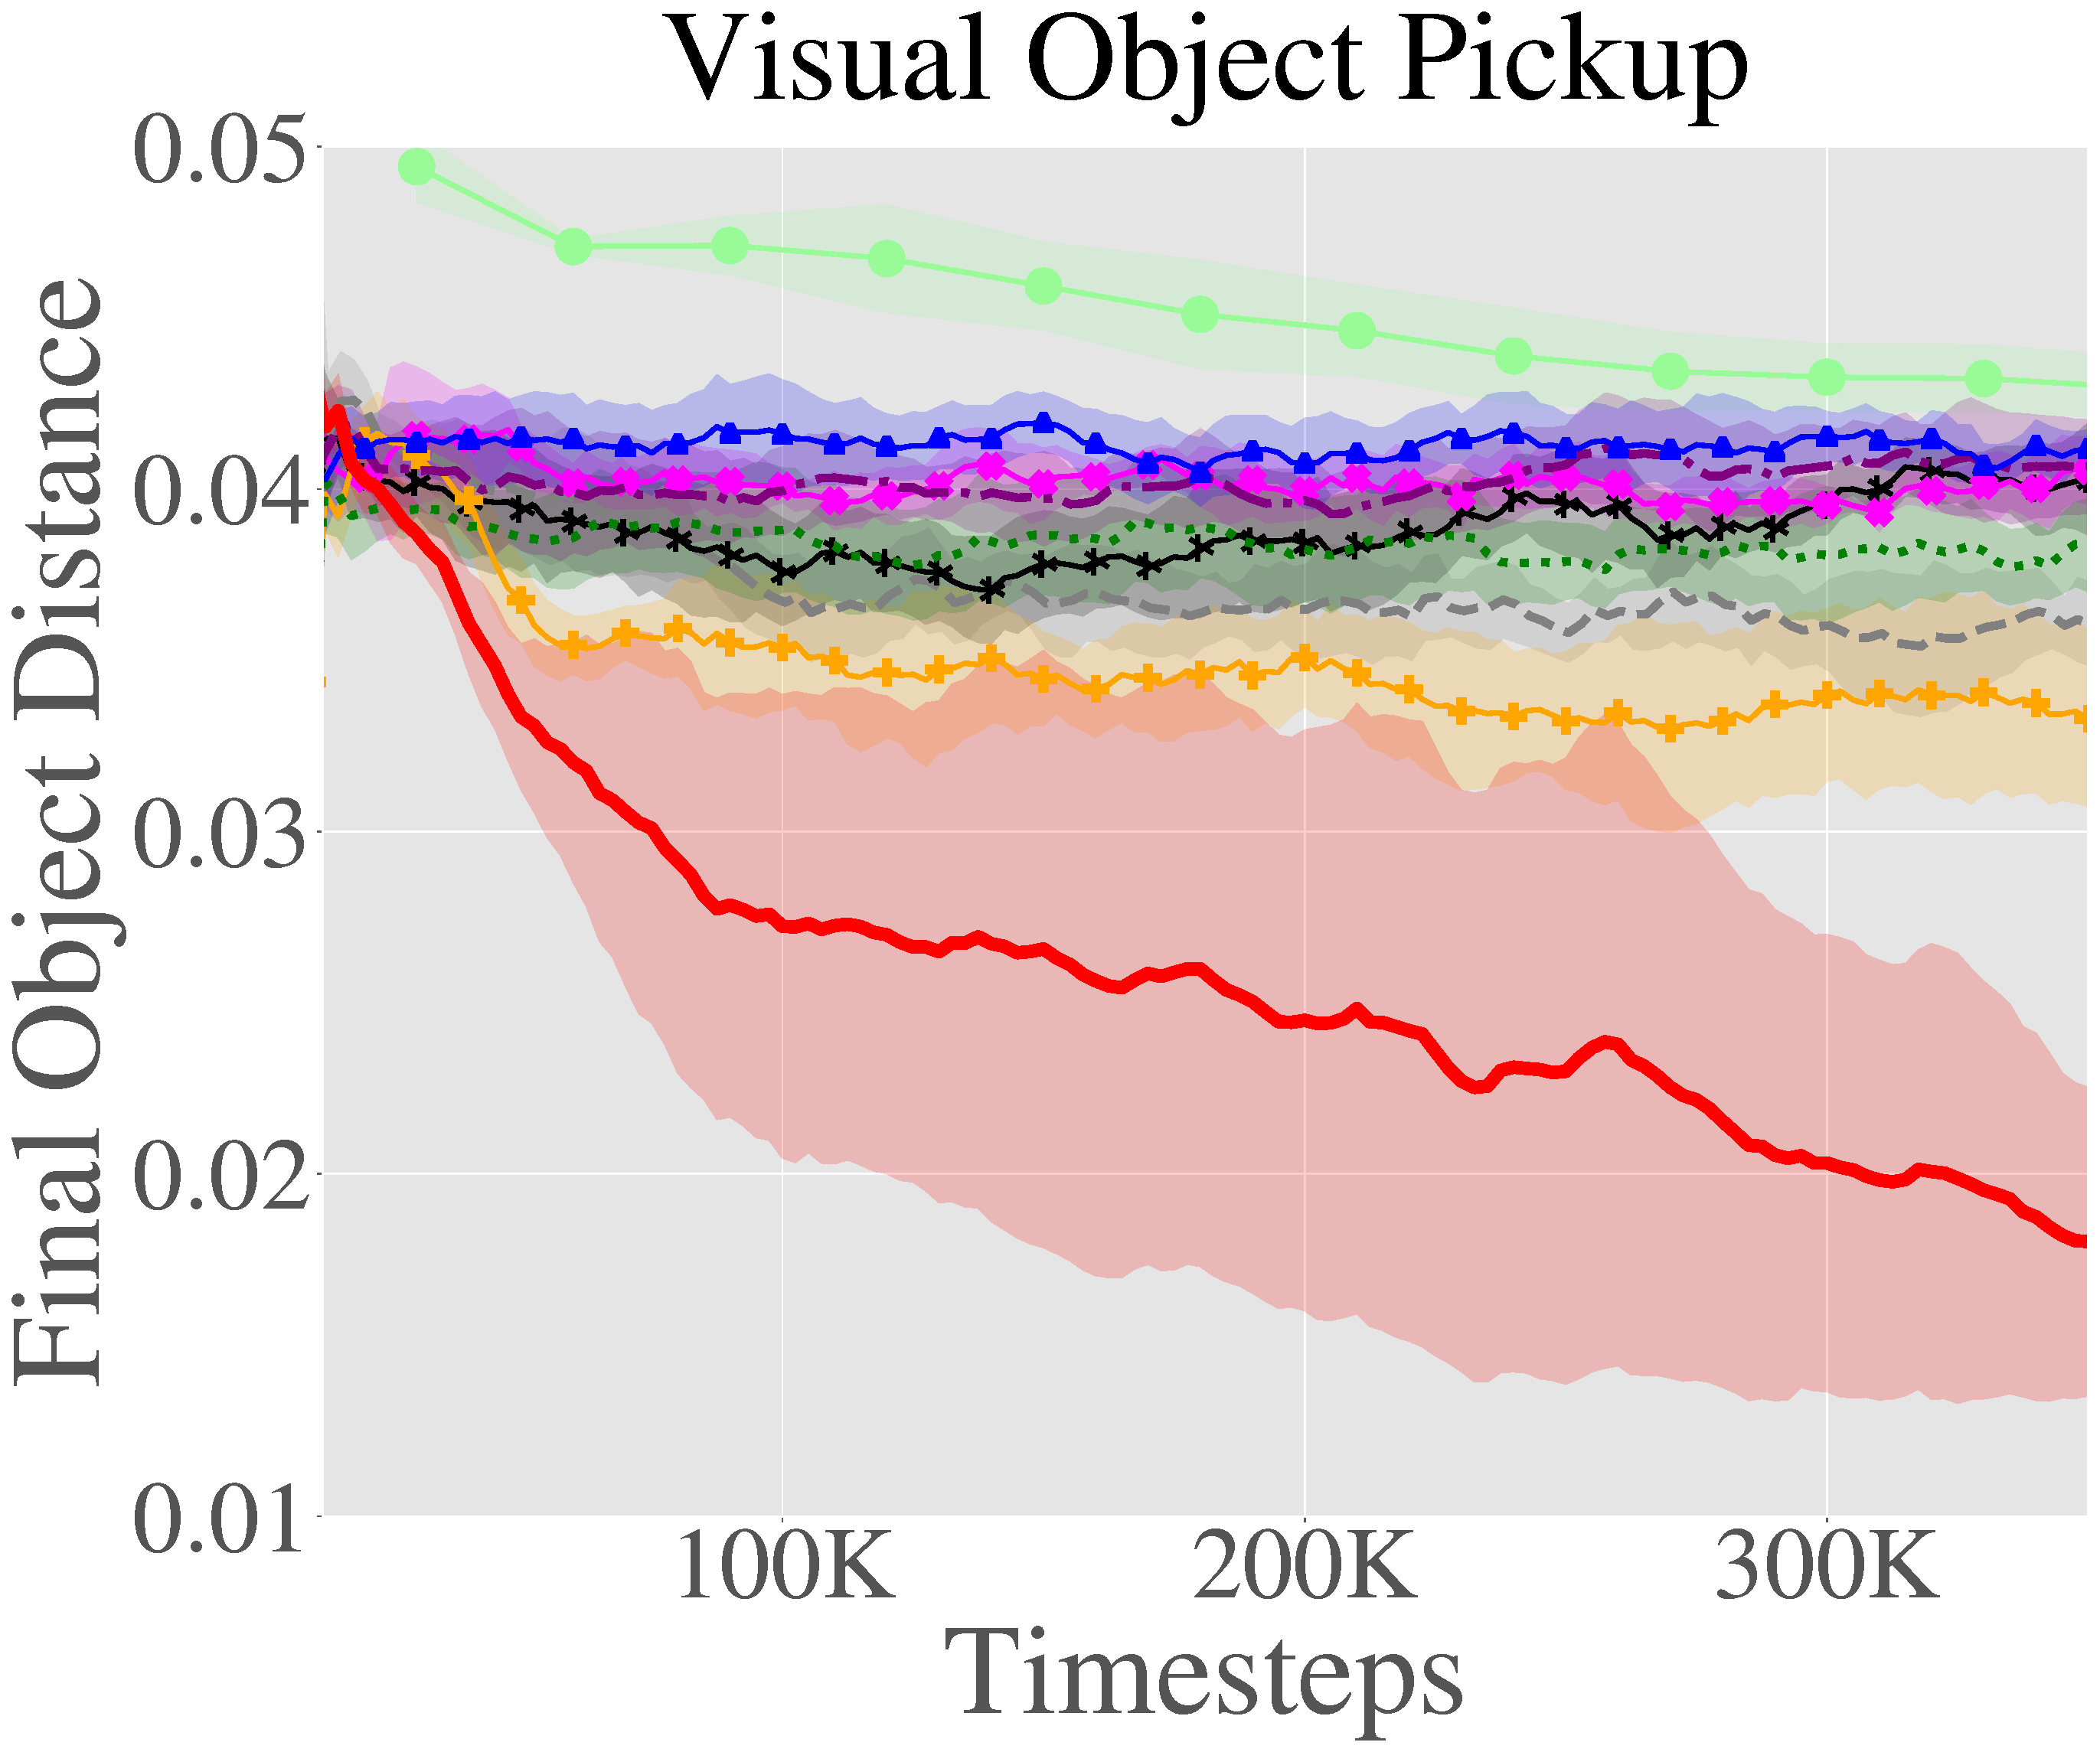
\includegraphics[width=\linewidth]{skewfit/figures/plots/main_sawyer_fig_with_hazan/pickup.pdf}
  \end{subfigure}

  \medskip

  \begin{subfigure}[t]{.49\linewidth}
    \centering
        %   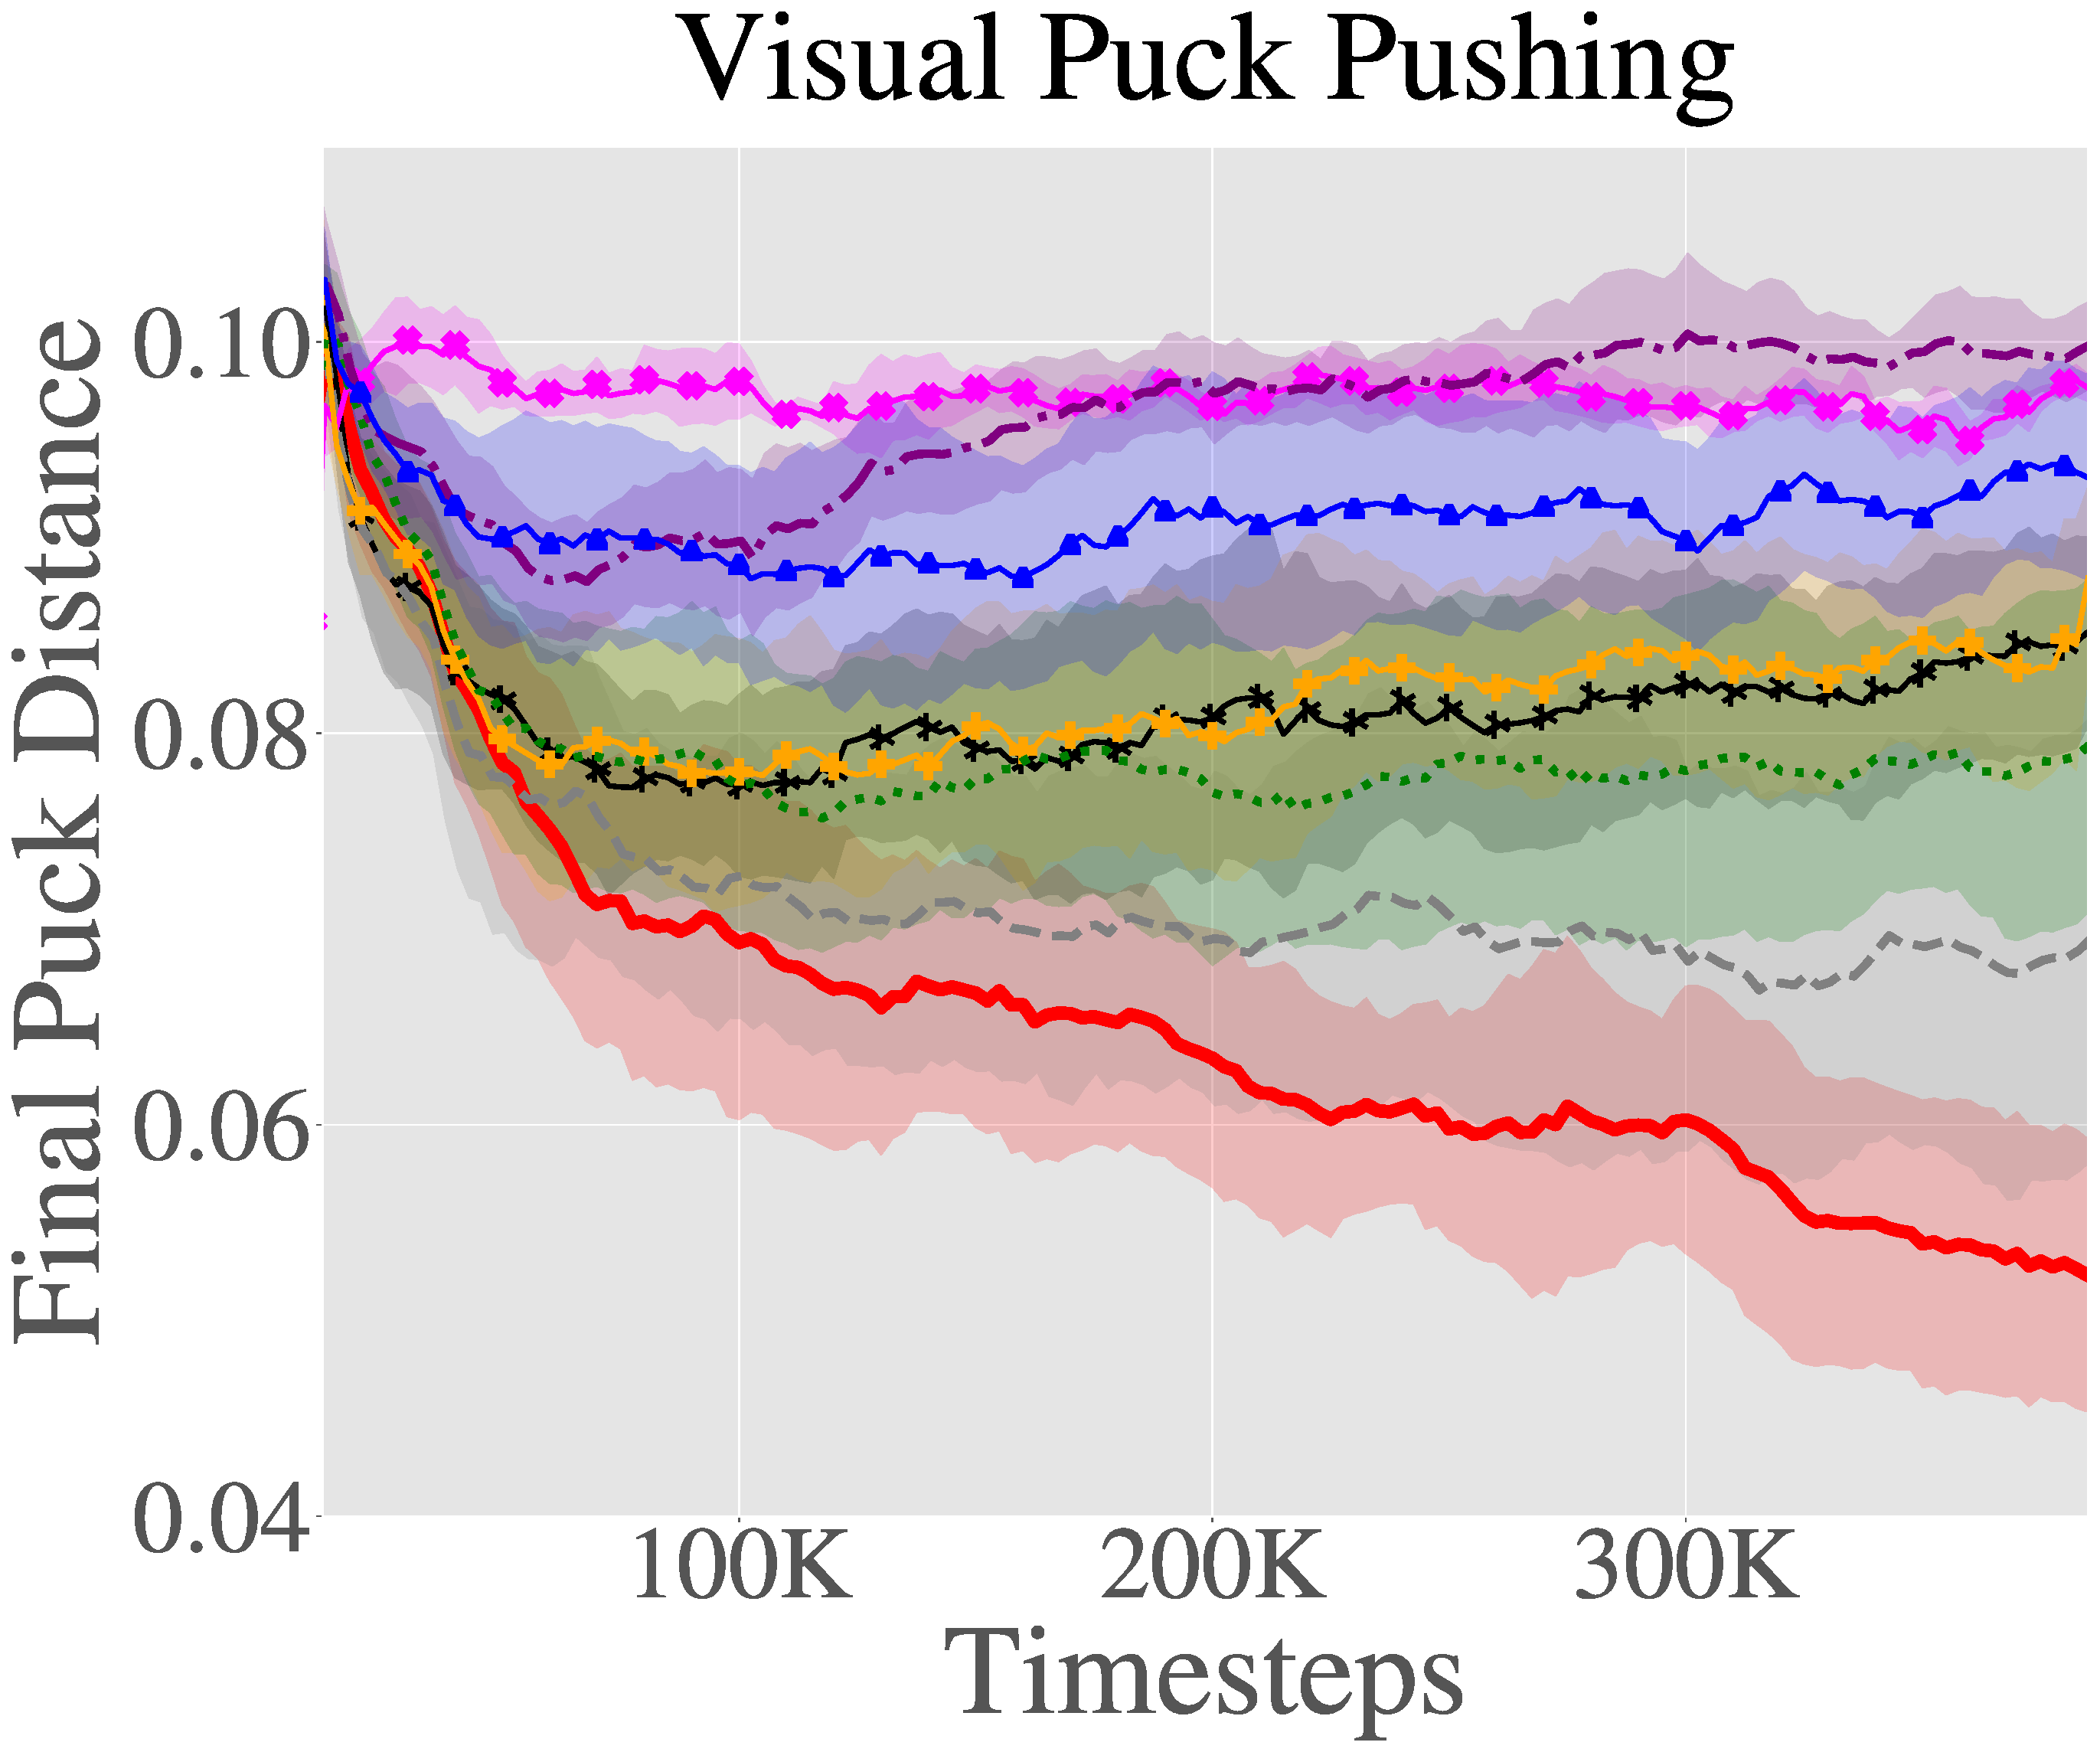
\includegraphics[width=\linewidth]{skewfit/figures/plots/main_sim_fig/pusher_big.pdf}
          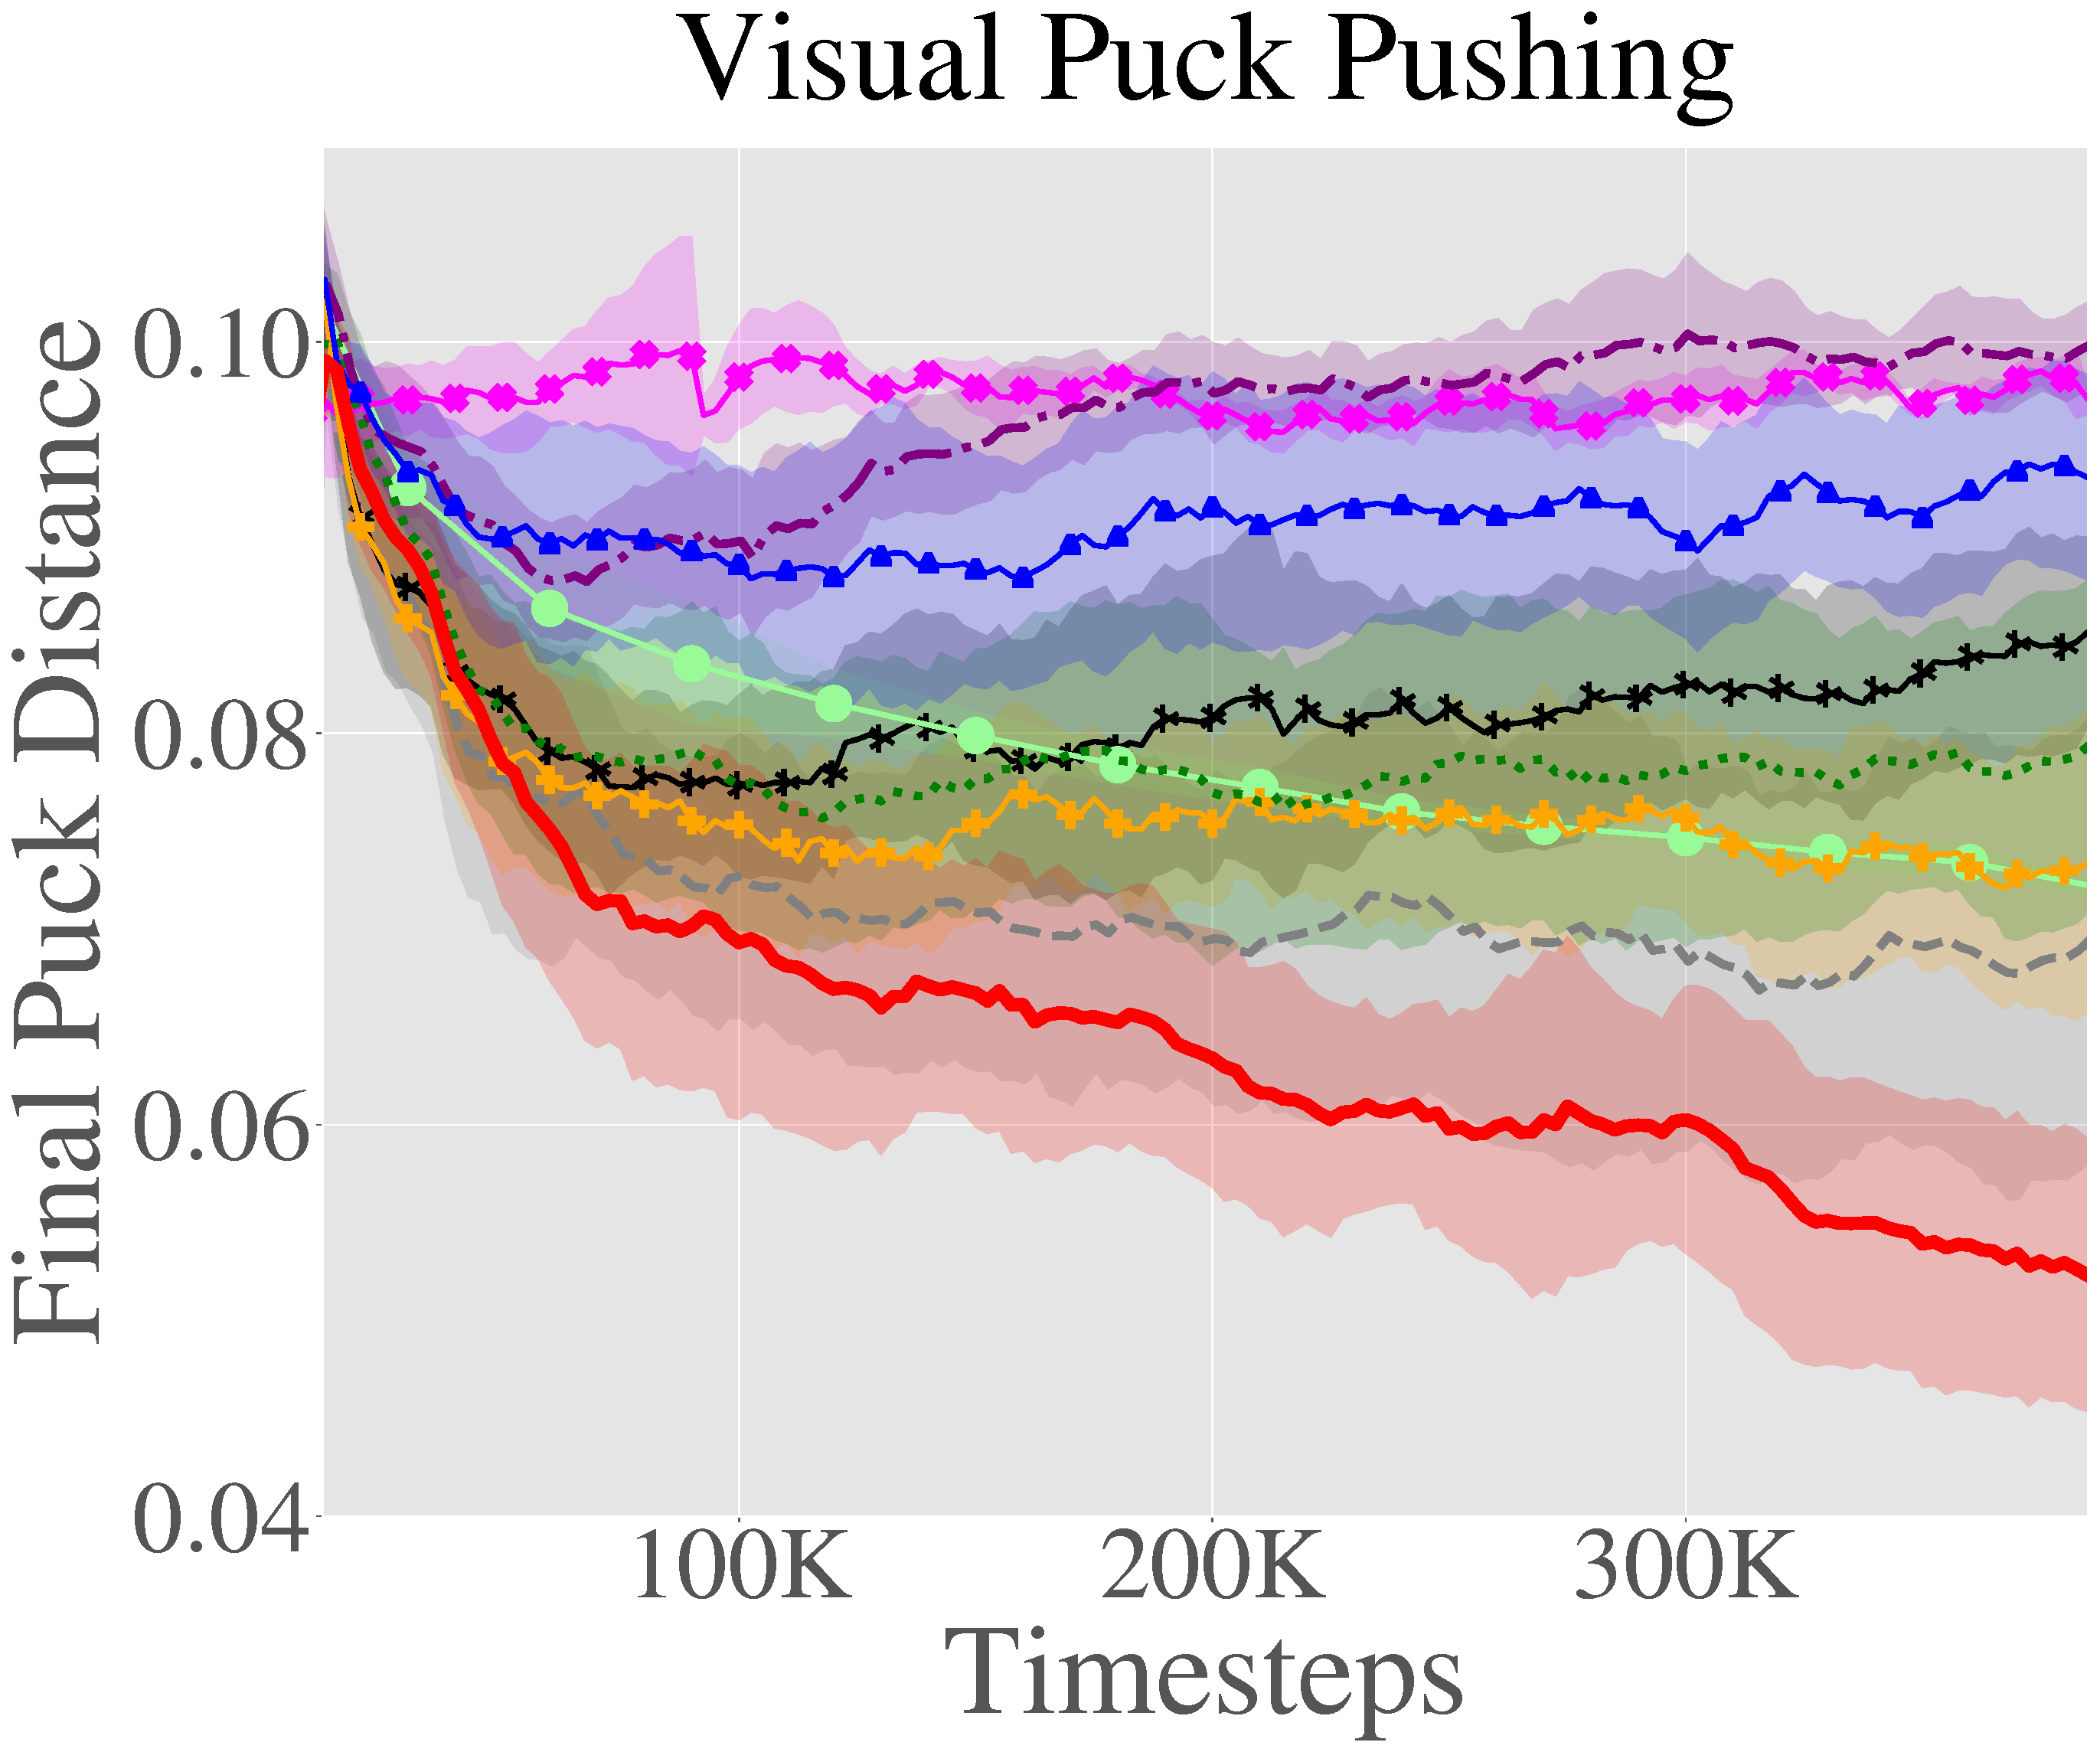
\includegraphics[width=\linewidth]{skewfit/figures/plots/main_sawyer_fig_with_hazan/pusher.pdf}
  \end{subfigure}
  \hfill
  \begin{subfigure}[t]{.48\linewidth}
    \centering
    % \hspace{0.165in}
    \raisebox{0.16in}{
        % 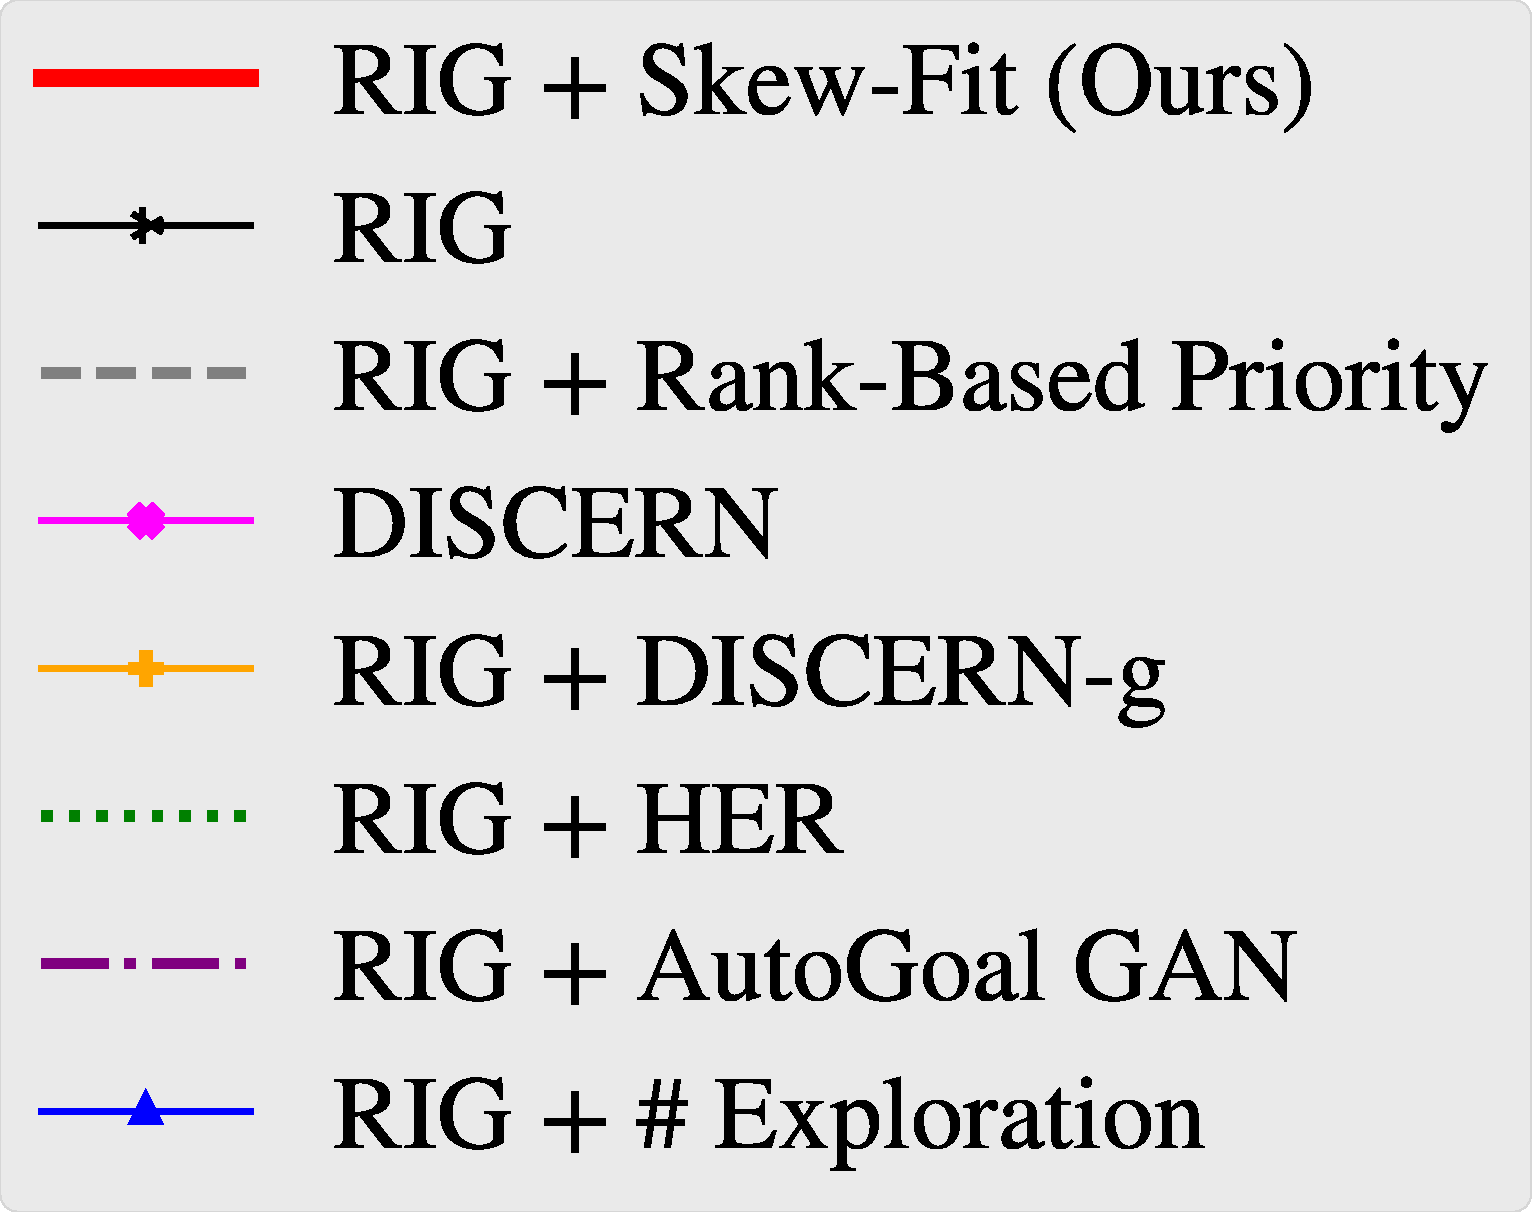
\includegraphics[width=0.8\linewidth]{skewfit/figures/plots/main_sim_fig/legend.pdf}
          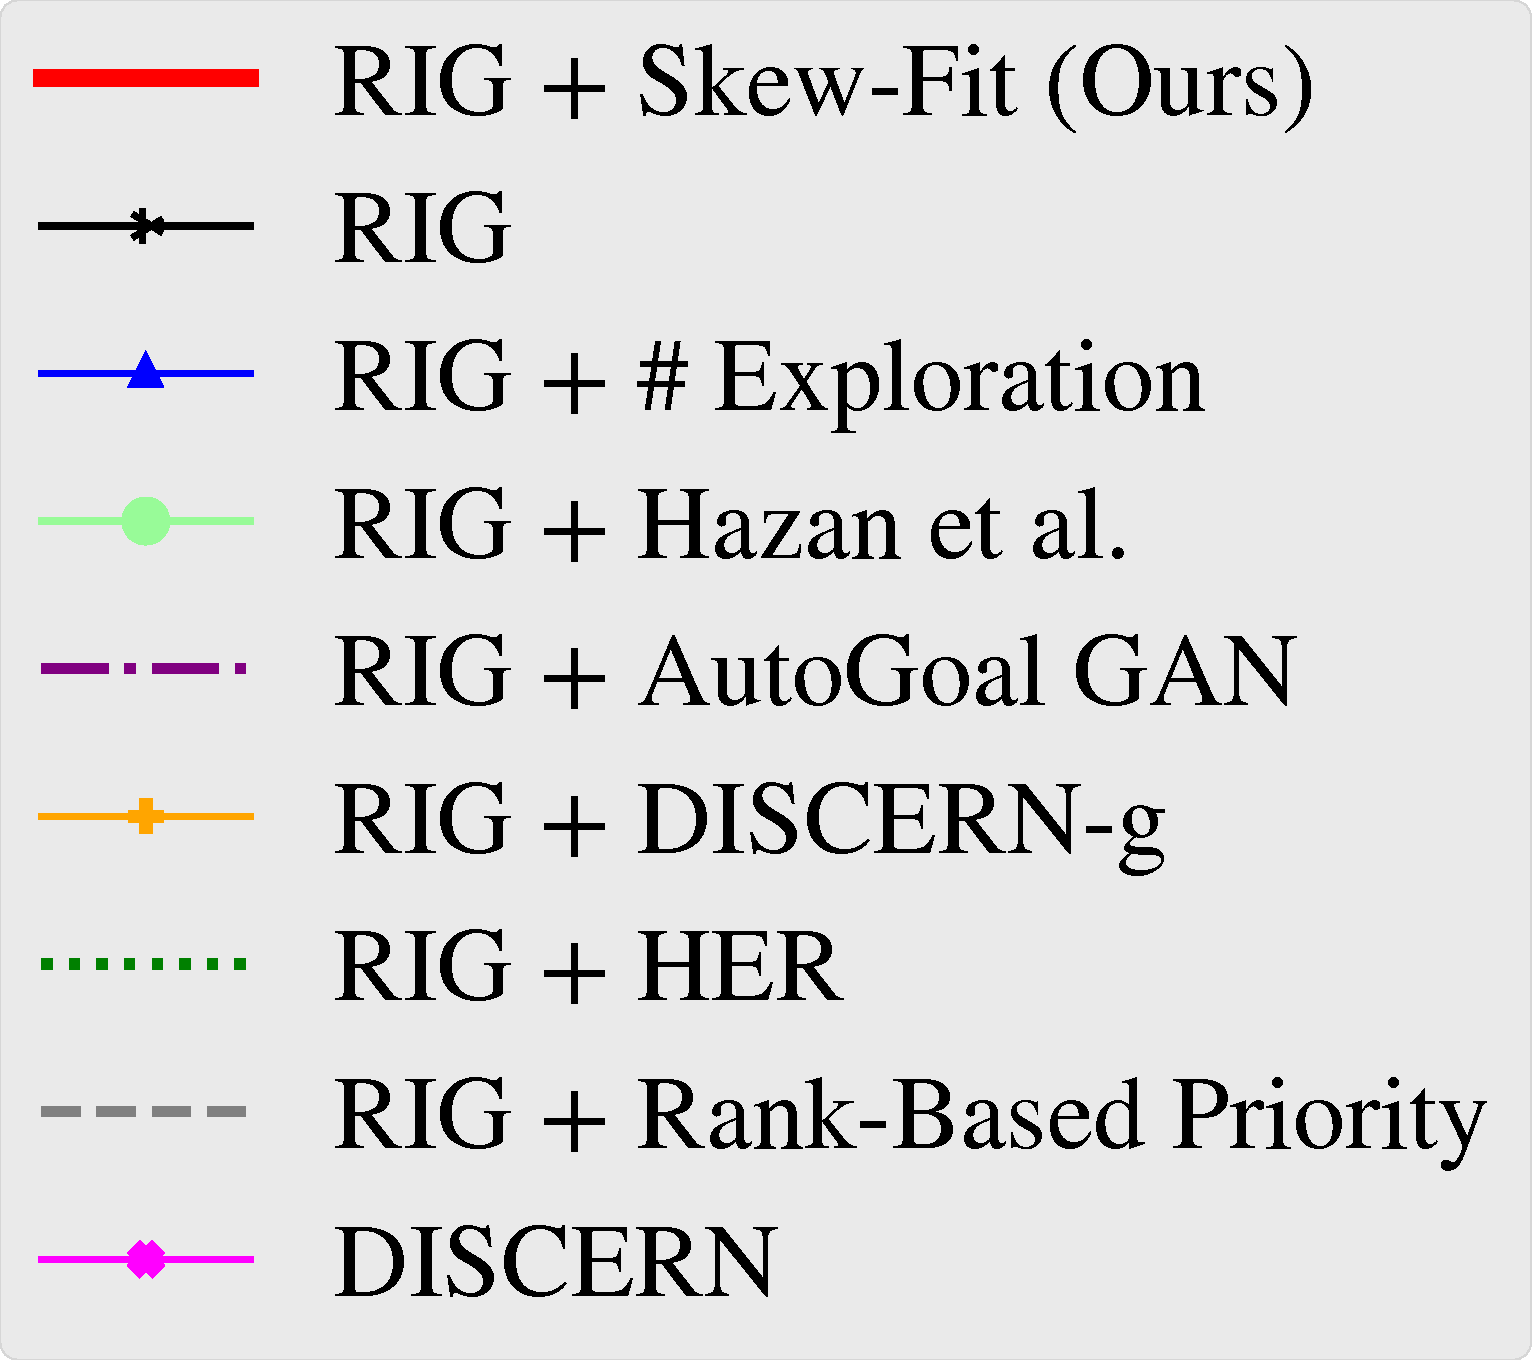
\includegraphics[width=\linewidth]{skewfit/figures/plots/main_sawyer_fig_with_hazan/main_figure_legend_with_hazan.pdf}
    }
  \end{subfigure}
    \fcaption{
        Learning curves for simulated continuous control tasks.
        Lower is better.
        We show the mean and standard deviation of 6 seeds and smooth temporally across 50 epochs within each seed.
        \METHOD consistently outperforms RIG and various prior methods.
        See text for description of each method.
    }
    \label{fig:sim-results}
\end{figure}


We see in \Figref{fig:sim-results} that Skew-Fit significantly outperforms prior methods both in terms of task performance and sample complexity.
The most common failure mode for prior methods is that the goal distributions collapse, resulting in the agent learning to reach only a fraction of the state space, as shown in \autoref{fig:offline-sk-real}.
For comparison, additional samples of $\pg$ when trained with and without \METHOD are shown in \autoref{sec:vae-dump}.
Those images show that without \METHOD, $\pg$ produces a small, non-diverse distribution for each environment: the object is in the same place for pickup, the puck is often in the starting position for pushing, and the door is always closed.
In contrast, \METHOD proposes goals where the object is in the air and on the ground, where the puck positions are varied, and the door angle changes.

We can see the effect of these goal choices by visualizing more example rollouts for RIG and \METHOD.
These visuals, shown in \Figref{fig:example_rollouts} in \autoref{sec:vae-dump}, show that RIG only learns to reach states close to the initial position, while \METHOD learns to reach the entire state space.
For a quantitative comparison, \Figref{fig:exploration_pickups} shows the cumulative total exploration pickups for each method.
From the graph, we see that many methods have a near-constant rate of object lifts throughout all of training.
\METHOD is the only method that significantly increases the rate at which the policy picks up the object during exploration, suggesting that only \METHOD sets goals that encourage the policy to interact with the object.

\begin{figure}[t]
\centering
  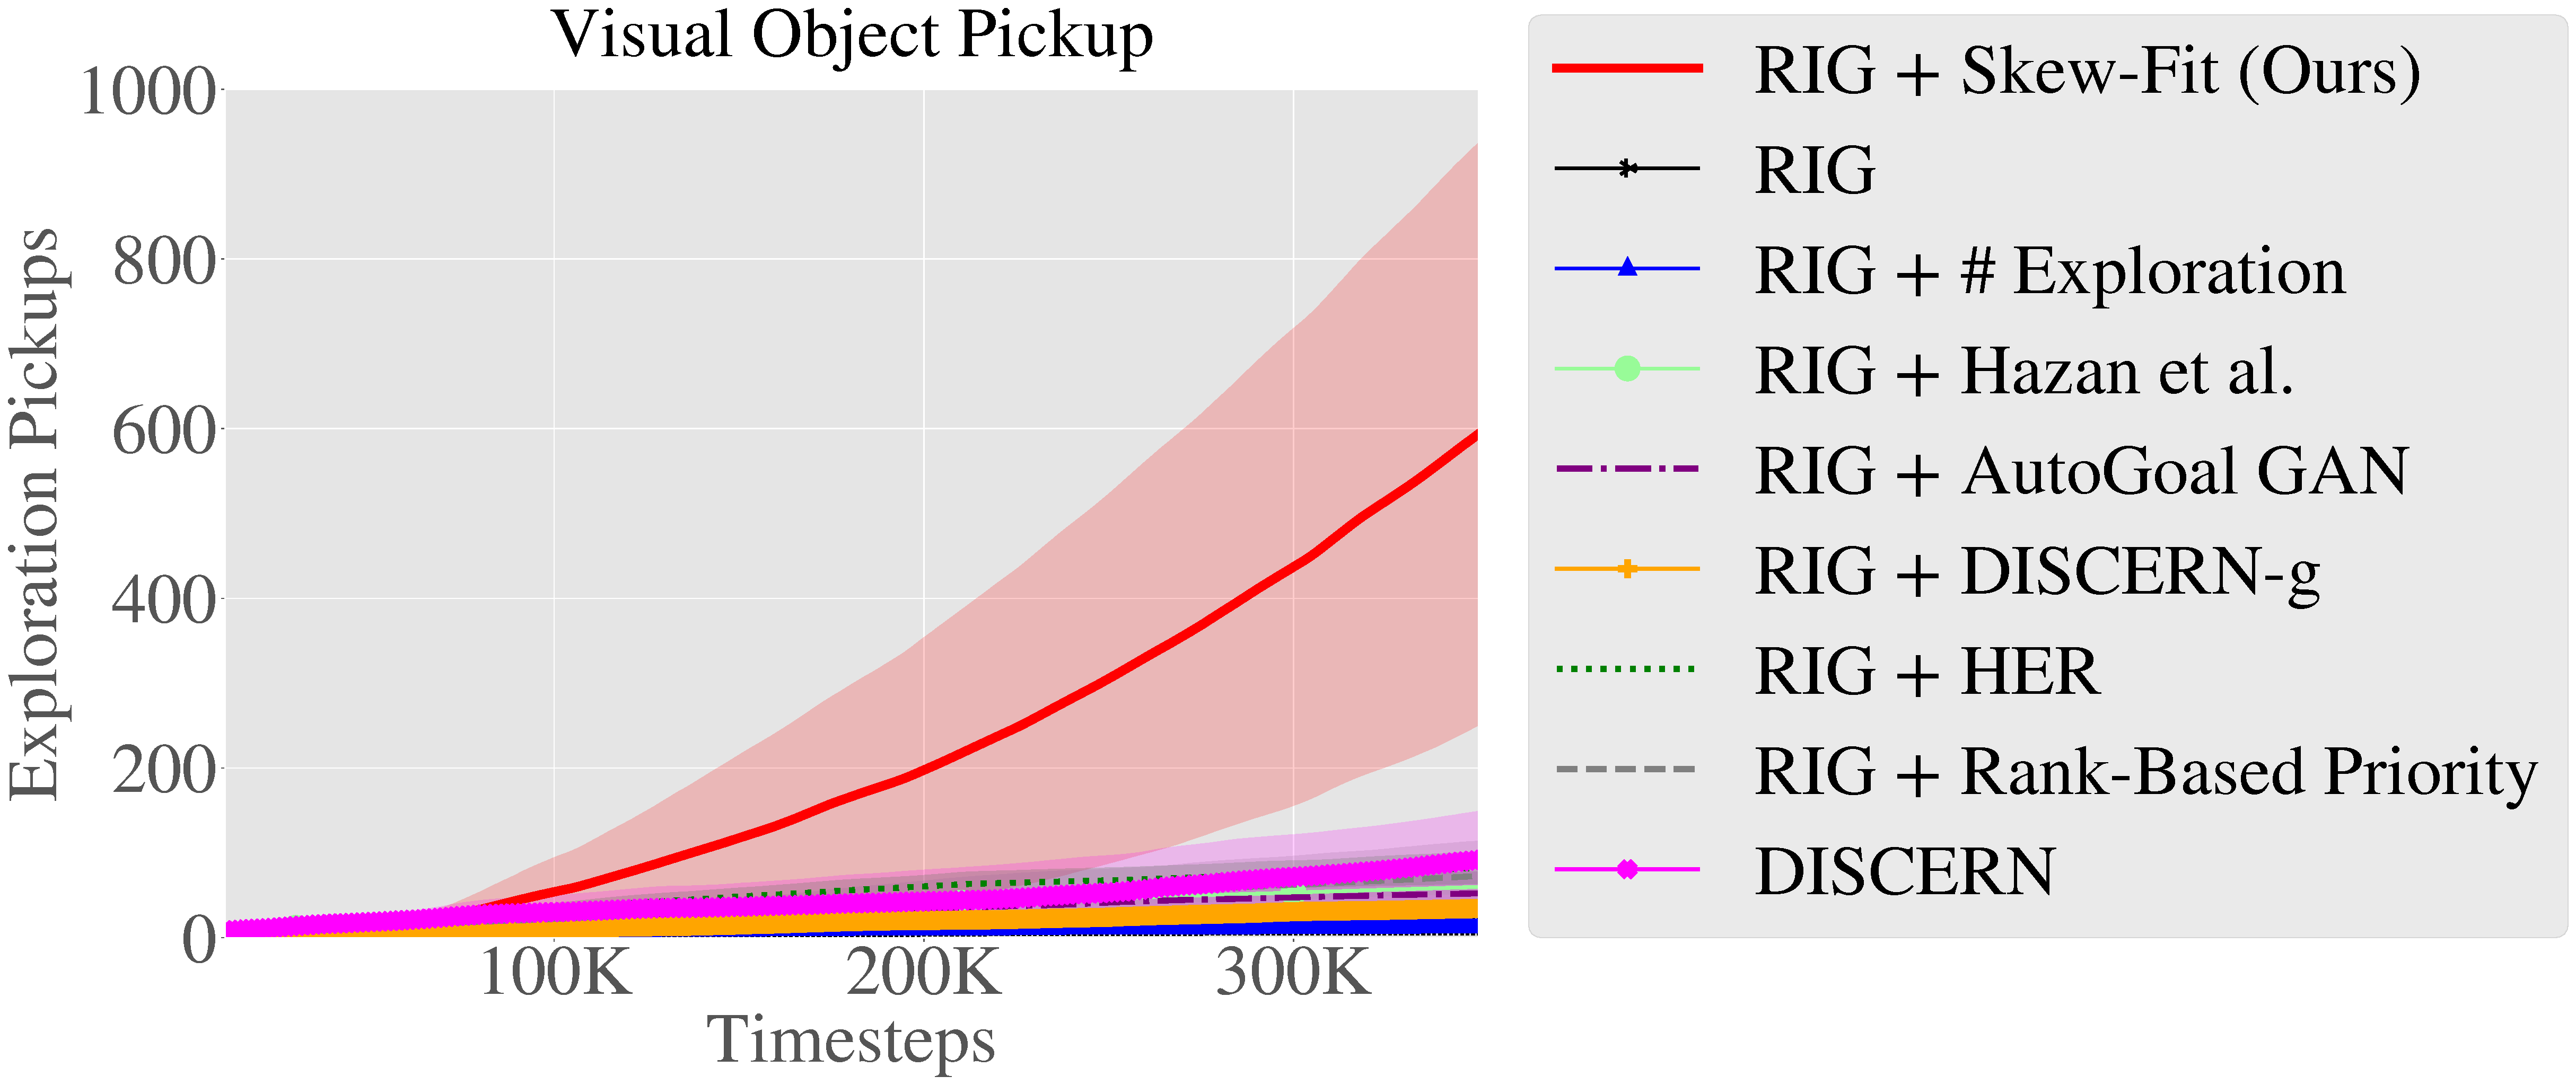
\includegraphics[width=\linewidth]{skewfit/figures/plots/exploration_pickups.pdf}
  \fcaption{
Cumulative total pickups during exploration for each method.
Prior methods fail to pay attention to the object: the rate of pickups hardly increases past the first 100 thousand timesteps.
In contrast, after seeing the object picked up a few times, \METHOD practices picking up the object more often by sampling the appropriate exploration goals.
}
  \label{fig:exploration_pickups}
\end{figure}


\paragraph{Real-World Vision-Based Robotic Manipulation}
We also demonstrate that \METHOD scales well to the real world with a door opening task, \textit{Real World Visual Door}, as shown in \Figref{fig:env-pics}.
While a number of prior works have studied RL-based learning of door opening~\cite{kalakrishnan2011learning,chebotar2017path}, we demonstrate the first method for autonomous learning of door opening without a user-provided, task-specific reward function.
As in simulation, we do not provide any goals to the agent and simply let it interact with the door, without any human guidance or reward signal.
We train two agents using RIG and RIG with \METHOD.
Every seven and a half minutes of interaction time, we evaluate on $5$ goals and plot the cumulative successes for each method.
Unlike in simulation, we cannot easily measure the difference between the policy's achieved and desired door angle.
Instead, we visually denote a binary success/failure for each goal based on whether the last state in the trajectory achieves the target angle.
As \Figref{fig:real-results} shows, standard RIG only starts to open the door after five hours of training.
In contrast, \METHOD learns to occasionally open the door after three hours of training and achieves a near-perfect success rate after five and a half hours of interaction.
\autoref{fig:real-results} also shows examples of successful trajectories from the \METHOD policy, where we see that the policy can reach a variety of user-specified goals.
These results demonstrate that \METHOD is a promising technique for solving real world tasks without any human-provided reward function.
Videos of \METHOD solving this task and the simulated tasks can be viewed on
our website.
\footnote{https://sites.google.com/view/skew-fit}

\begin{figure}[t]
  \centering
  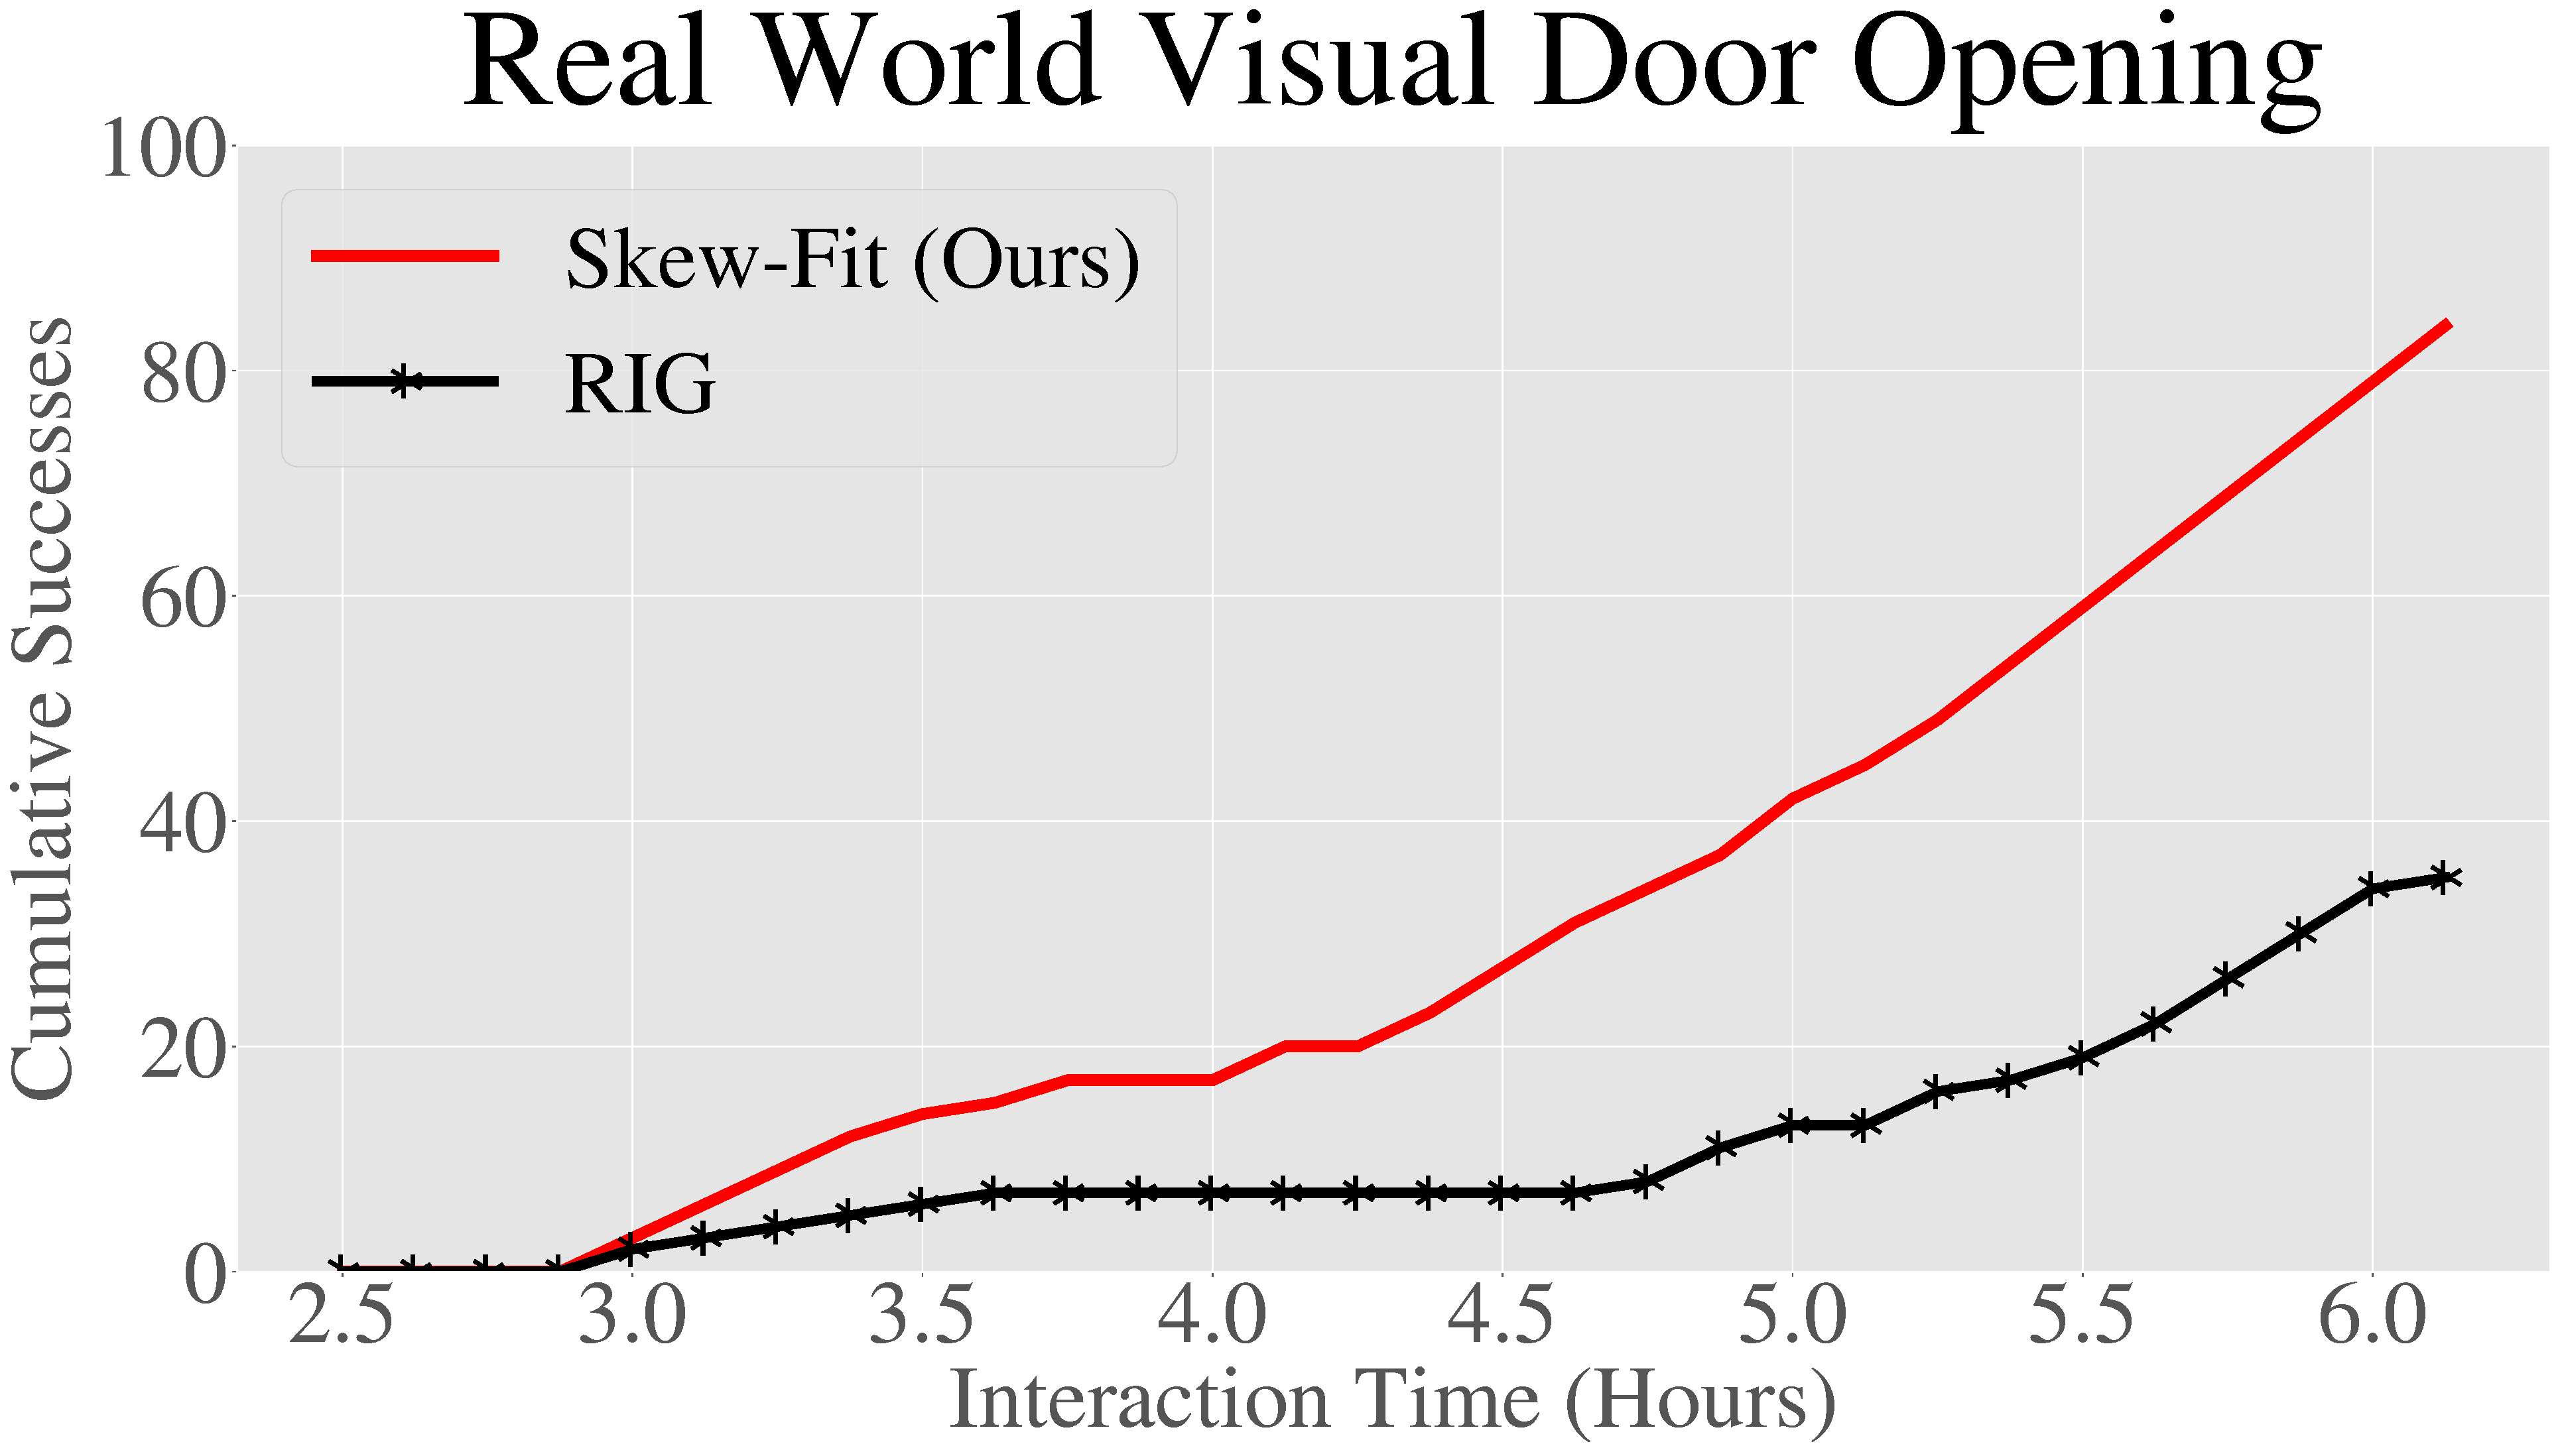
\includegraphics[width=0.75\linewidth]{skewfit/figures/plots/real_world_door.pdf}
    \begin{subfigure}[b]{0.49\textwidth}
        \center
        \hspace{-.2cm}
        $\SF_1$ \hspace{4.3cm} $\SF_{100}$ \hspace{.7cm} $\G$

        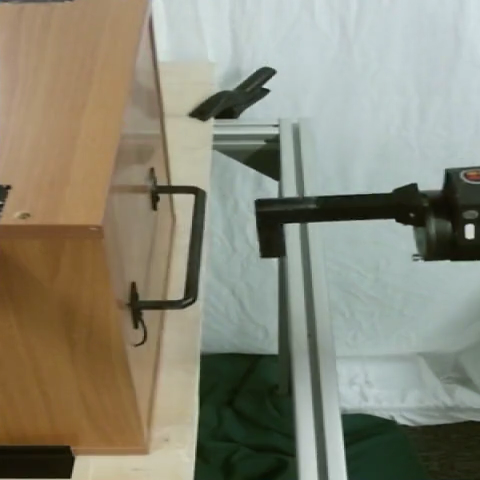
\includegraphics[width=0.14\linewidth]{skewfit/figures/imgs/real_env_rollout_new/door_easy/barely_open_5.png}
        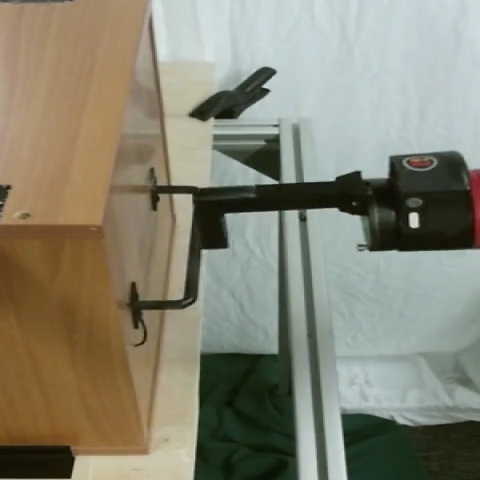
\includegraphics[width=0.14\linewidth]{skewfit/figures/imgs/real_env_rollout_new/door_easy/barely_open_10.png}
        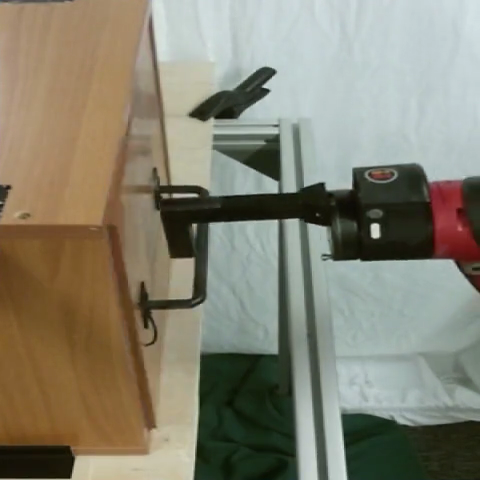
\includegraphics[width=0.14\linewidth]{skewfit/figures/imgs/real_env_rollout_new/door_easy/barely_open_15.png}
        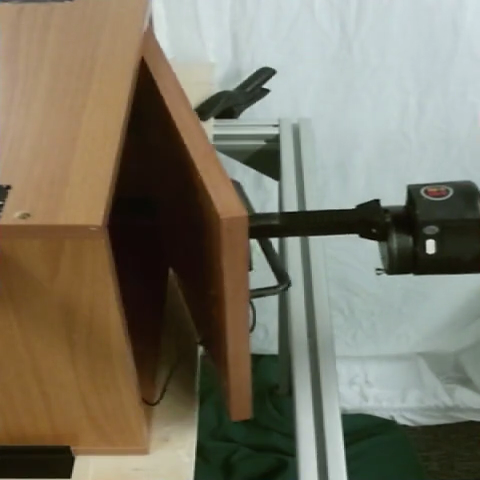
\includegraphics[width=0.14\linewidth]{skewfit/figures/imgs/real_env_rollout_new/door_easy/barely_open_20.png}
        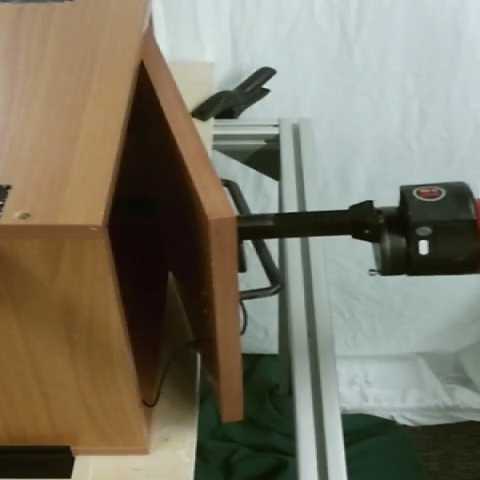
\includegraphics[width=0.14\linewidth]{skewfit/figures/imgs/real_env_rollout_new/door_easy/barely_open_25.png}
        \hspace{0.01\linewidth}
        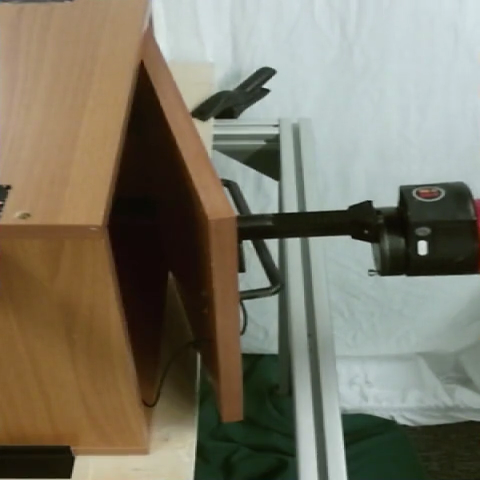
\includegraphics[width=0.14\linewidth]{skewfit/figures/imgs/real_env_rollout_new/door_easy/barely_open_45.png} %goal
    \end{subfigure}
    \begin{subfigure}[b]{0.49\textwidth}
        \center

        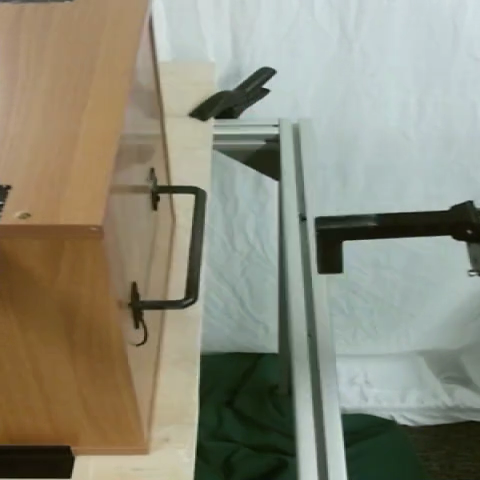
\includegraphics[width=0.14\linewidth]{skewfit/figures/imgs/real_env_rollout_novel/door_hard/wide_open_0.png}
        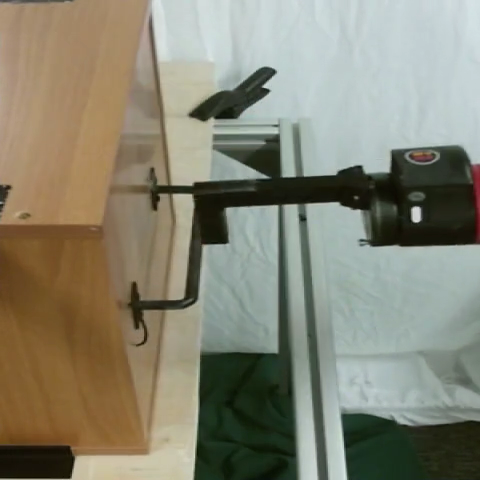
\includegraphics[width=0.14\linewidth]{skewfit/figures/imgs/real_env_rollout_novel/door_hard/wide_open_10.png}
        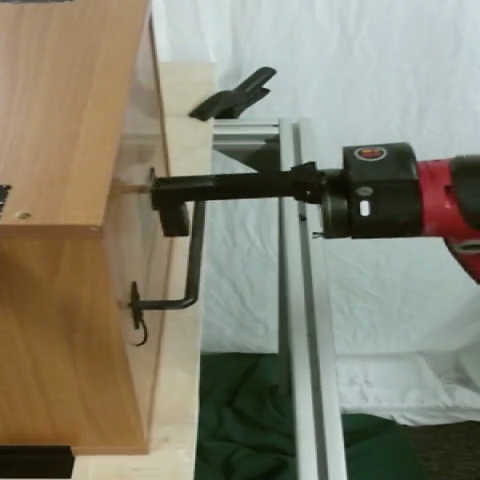
\includegraphics[width=0.14\linewidth]{skewfit/figures/imgs/real_env_rollout_novel/door_hard/wide_open_20.png}
        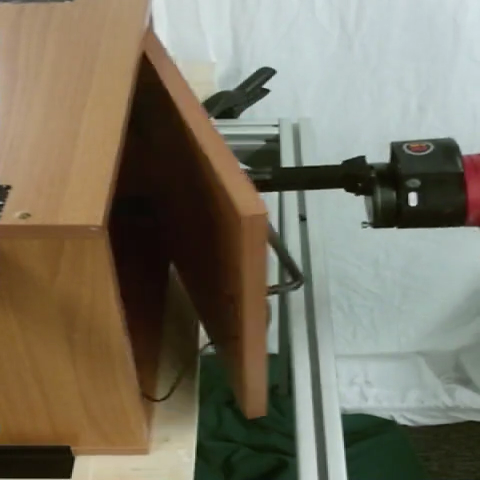
\includegraphics[width=0.14\linewidth]{skewfit/figures/imgs/real_env_rollout_novel/door_hard/wide_open_25.png}
        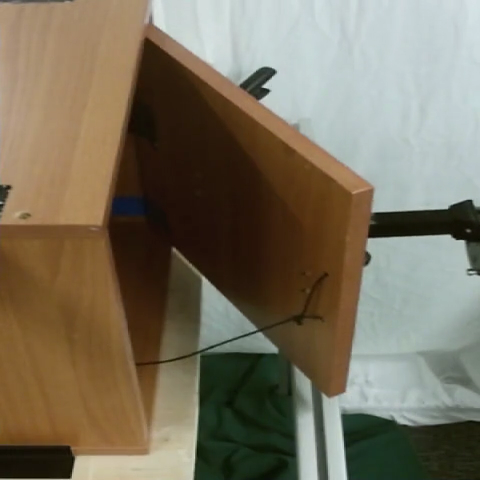
\includegraphics[width=0.14\linewidth]{skewfit/figures/imgs/real_env_rollout_novel/door_hard/wide_open_40.png}
        \hspace{0.01\linewidth}
        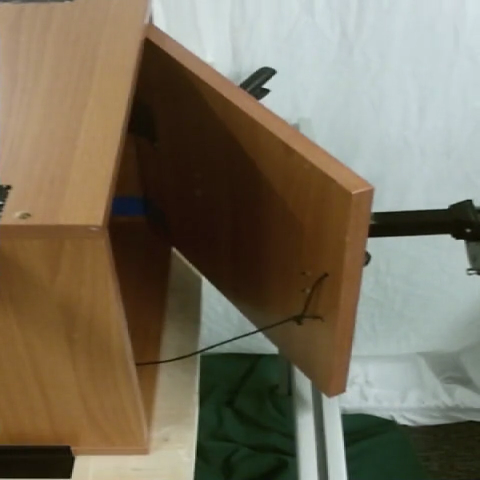
\includegraphics[width=0.14\linewidth]{skewfit/figures/imgs/real_env_rollout_novel/door_hard/wide_open_100.png}
    \end{subfigure}
  \fcaption{
  (Top) Learning curve for Real World Visual Door.
  \METHOD results in considerable sample efficiency gains over RIG on this real-world task.
  (Bottom)
  Each row shows the \METHOD policy starting from state $\SF_1$ and reaching state $\SF_{100}$ while pursuing goal $\G$.
  Despite being trained from only images without any user-provided goals during training, the \METHOD policy achieves the goal image provided at test-time, successfully opening the door.
  }
  \label{fig:real-results}
\end{figure}



\paragraph{Additional Experiments}
To study the sensitivity of \METHOD to the hyperparameter $\alpha$, we sweep $\alpha$ across the values $[-1, -0.75, -0.5, -0.25, 0]$ on the simulated image-based tasks.
The results are in \autoref{sec:add-exps} and demonstrate that \METHOD works across a large range of values for $\alpha$, and $\alpha=-1$ consistently outperform $\alpha=0$ (i.e. outperforms no \METHOD).
Additionally, \autoref{sec:implementation-details} provides a complete description our method hyperparameters, including network architecture and RL algorithm hyperparameters.

\section{Conclusion}\label{sec:conclusion}
We presented a formal objective for self-supervised goal-directed exploration, allowing researchers to quantify and compare progress when designing algorithms that enable agents to autonomously learn.
We also presented \METHOD, an algorithm for training a generative model to approximate a uniform distribution over an initially unknown set of valid states, using data obtained via goal-conditioned reinforcement learning, and our theoretical analysis gives conditions under which \METHOD converges to the uniform distribution.
When such a model is used to choose goals for exploration and to relabeling goals for training, the resulting method results in much better coverage of the state space, enabling our method to explore effectively.
Our experiments show that when we concurrently train a goal-reaching policy using self-generated goals, \METHOD produces quantifiable improvements on simulated robotic manipulation tasks, and can be used to learn a door opening skill to reach a $95\%$ success rate directly on a real-world robot, without any human-provided reward supervision.

\section{Contribution Statement}

The work in this chapter was performed in collaboration with Vitchyr Pong, Murtaza Dalal, Steven Lin, Shikhar Bahl, and Sergey Levine~\cite{pong2019skewfit}. The idea of self-supervised goal setting with an expanding goal space by iteratively retraining a generative model was developed jointly by Vitchyr and Ashvin. Vitchyr conducted the theoretical analysis, and managed the project, and led the writing of the paper. The simulation experiments were conducted by Vitchyr, Murtaza, and Steven. Vitchyr, Murtaza, Ashvin, and Shikhar conducted the real world experiments. Ashvin assisted with writing and analysis. Sergey Levine advised on the project, guided the theoretical analysis, and assisted with writing.

{\small
\bibliographystyle{corlabbrvnat}
\bibliography{main.bib}
}

\clearpage
\newpage
\noindent\makebox[\linewidth]{\rule{\linewidth}{3.0pt}}
\begin{center}
\LARGE{\textbf{Supplementary Material}}
\end{center}
\noindent\makebox[\linewidth]{\rule{\linewidth}{0.8pt}}

\section{Complete Ablative Results} \label{sec:appendix}

\subsection{Relabeling strategy ablation} \label{sec:appendix_relabeling_ablation}

In this experiment, we compare different goal resampling strategies for training the Q function. We consider:
\textit{Future},
relabeling the goal for a transition by sampling uniformly from future states in the trajectory as done in \citet{andrychowicz2017her};
\textit{VAE}, sampling goals from the VAE only;
\textit{RIG}, relabeling goals with probability $0.5$ from the VAE and probability $0.5$ using the future strategy;
and \textit{None}, no relabeling. 
Figure \ref{fig:relabel-ablation-all-envs} shows the effect of different relabeling strategies with our method.

\begin{figure}[h]
    \centering
    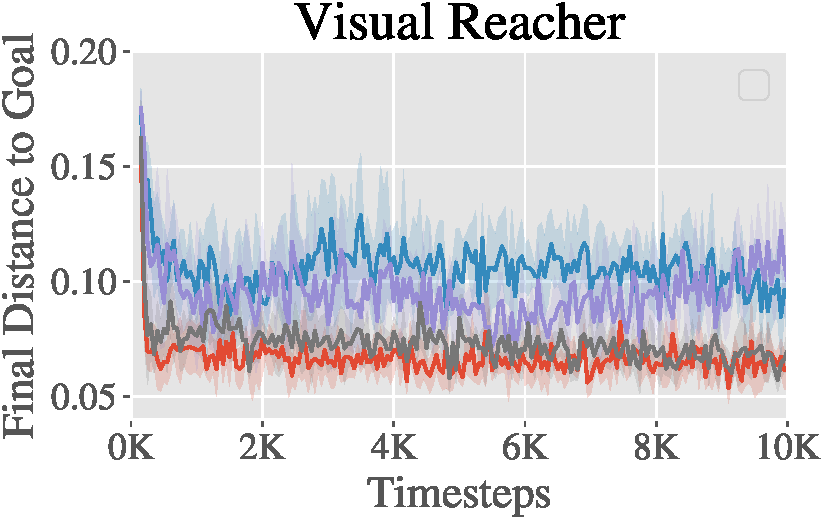
\includegraphics[height=0.185\linewidth]{img/reacher_relabeling_ablation.pdf}
    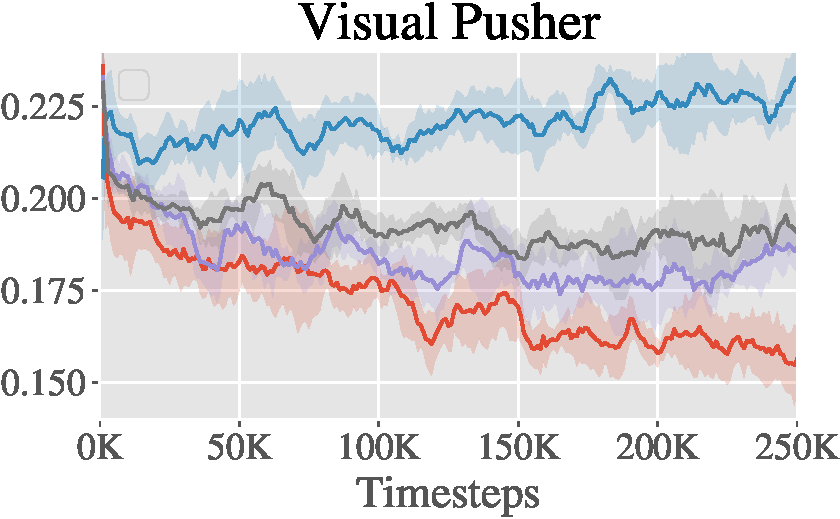
\includegraphics[height=0.185\linewidth]{img/pusher_relabeling_ablation.pdf}
    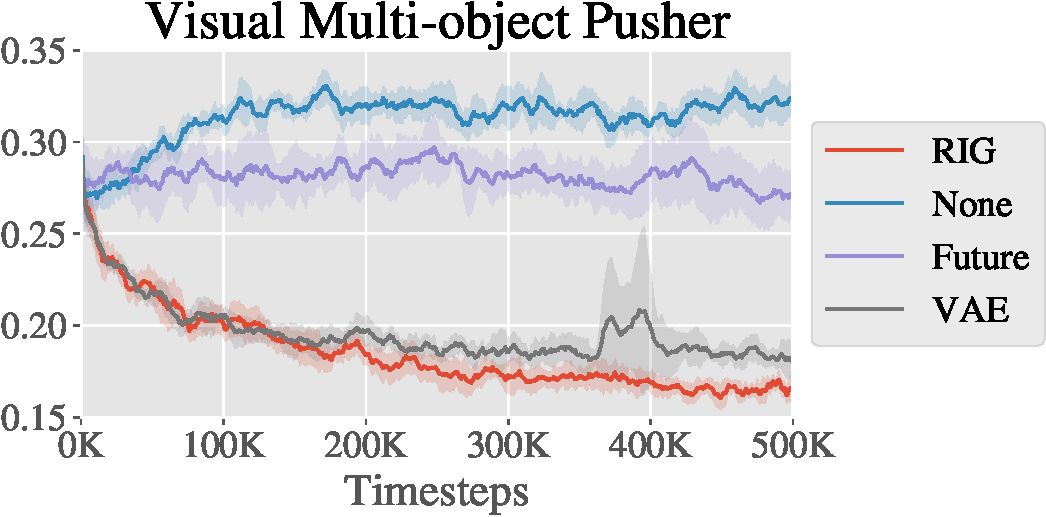
\includegraphics[height=0.185\linewidth]{img/multiobj_pusher_relabeling_ablation.pdf}
    \caption{Relabeling ablation simulated results, showing final distance to goal vs environment steps. RIG (red), which uses a mixture of VAE and future, consistently matches or outperforms the other methods.}
    \vspace{-0.1in}
    \label{fig:relabel-ablation-all-envs}
\end{figure}

\subsection{Reward type ablation}

In this experiment, we change only the reward function that we use to train the goal-conditioned valued function to show the effect of using the latent distance reward.
We include the following methods for comparison:
\textit{Latent Distance}, which is the reward used in RIG, i.e. $A = \mathbf{I}$ in Equation \eqref{eq:reward-log-prob-equivalence};
\textit{Log Probability}, which uses the Mahalanobis distance in Equation \eqref{eq:reward-log-prob-equivalence}, where $A$ is the precision matrix of the encoder;
and \textit{Pixel MSE}, which computes mean-squared error (MSE) between state and goal in pixel space. To compute the pixel MSE for a sampled latent goal, we decode the goal latent using the VAE decoder, $p_\psi$, to generate the corresponding goal image. Figure \ref{fig:reward-ablation-all-envs} shows the effect of different rewards with our method.

\begin{figure}[h]
    \centering
    % \includegraphics[height=0.25\linewidth]{img/reacher_reward_type_ablation_b.pdf}
    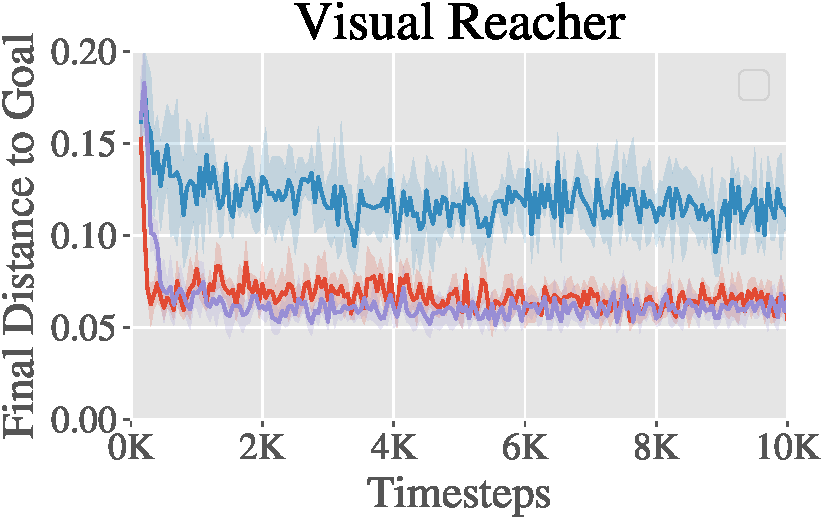
\includegraphics[height=0.19\linewidth]{img/reacher_reward_type_ablation.pdf}
    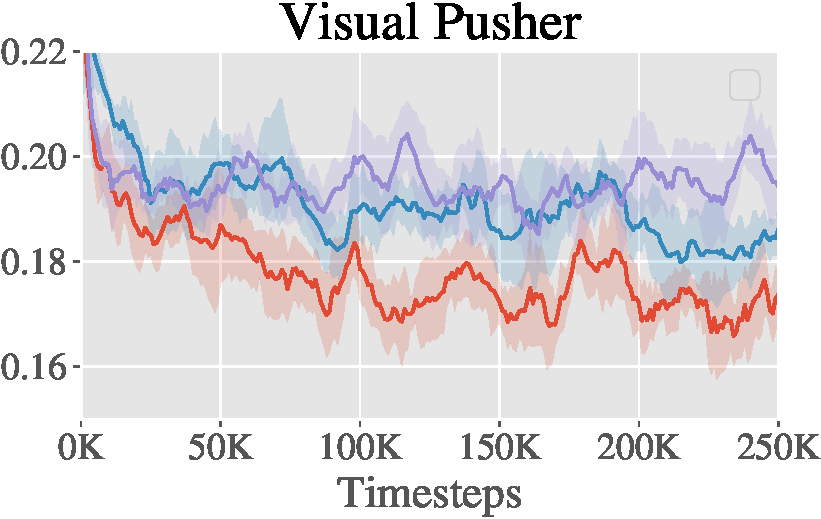
\includegraphics[height=0.19\linewidth]{img/pusher_reward_type_ablation.pdf}
    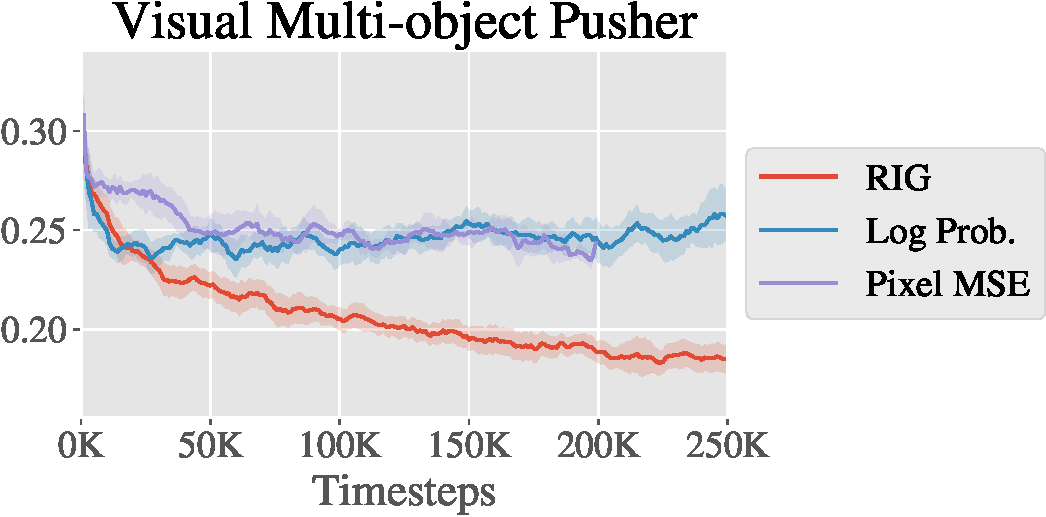
\includegraphics[height=0.19\linewidth]{img/multiobj_pusher_reward_type_ablation.pdf}
    \caption{Reward type ablation simulated results, showing final distance to goal vs environment steps. RIG (red), which uses latent distance for the reward, consistently matches or outperforms the other reward types.}
    \vspace{-0.1in}
    \label{fig:reward-ablation-all-envs}
\end{figure}

\subsection{Online training ablation} \label{sec:appendix_online}
Rather than pre-training the VAE on a set of images collected by a random policy, here we train the VAE in an online manner: the VAE is not trained when we initially collect data with our policy.
After every 3000 environment steps, we train the VAE on all of the images observed by the policy.
We show in Figure \ref{fig:online-ablation-all-envs} that this online training results in a good policy and is substantially better than leaving the VAE untrained.
These results show that the representation learning can be done simultaneously as the reinforcement learning portion of RIG, eliminating the need to have a predefined set of images to train the VAE.

The Visual Pusher experiment for this ablation is performed on a slightly easier version of the Visual Pusher used for the main results.
In particular, the goal space is reduced to be three quarters of its original size in the lateral dimension.

\begin{figure}[h]
    \centering
    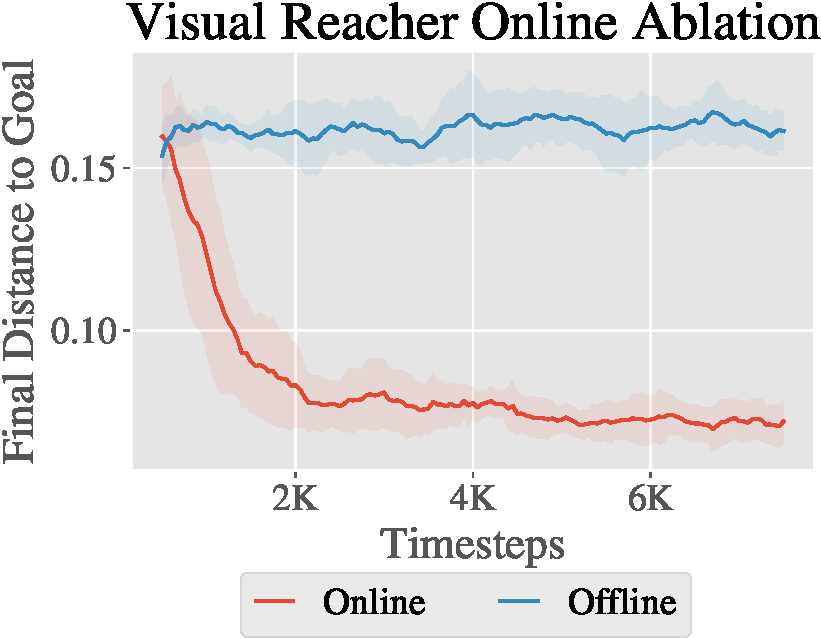
\includegraphics[height=0.2\linewidth]{img/reacher_online_ablation.pdf}
    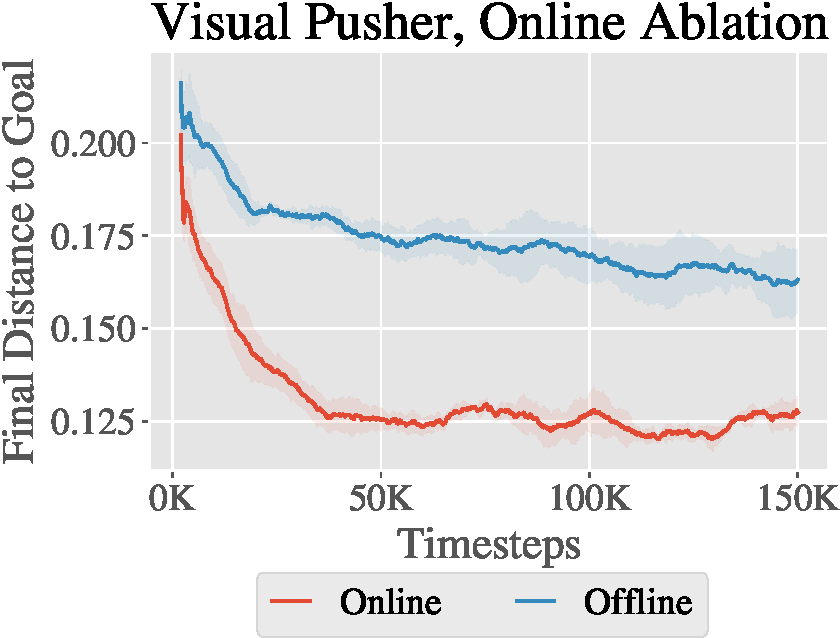
\includegraphics[height=0.2\linewidth]{img/pusher_online_ablation.pdf}
    \caption{Online vs offline VAE training ablation simulated results, showing final distance to goal vs environment steps. Given no pre-training phase, training the VAE online (red), outperforms no training of the VAE, and also performs well.}
    \vspace{-0.1in}
    \label{fig:online-ablation-all-envs}
\end{figure}

\subsection{Comparison to Hindsight Experience Replay} \label{sec:her_relabeling_ablation}

In this section, we study in isolation the effect of sampling goals from the goal space directly for Q-learning, as covered in Section~\ref{sec:goal-relabeling}.
Like hindsight experience replay \cite{andrychowicz2017her}, in this section we assume access to state information and the goal space, so we do not use a VAE.

To match the original work as closely as possible, this comparison was based off of the OpenAI baselines code \cite{plappert2018techreport} and we compare on the same Fetch robotics tasks. To minimize sample complexity and due to computational constraints, we use single threaded training with \texttt{rollout\_batch\_size=1, n\_cycles=1, batch\_size=256}. For testing, \texttt{n\_test\_rollouts=1} and the results are averaged over the last 100 test episodes. Number of updates per cycle corresponds to \texttt{n\_batches}.

On the plots, ``Future'' indicates
the future strategy as presented in \citet{andrychowicz2017her} with $k=4$. ``Ours'' indicates
resampling goals with probability 0.5 from the "future" strategy with $k=4$ and probability 0.5 uniformly from the environment goal space. Each method is shown with dense and sparse rewards.

\begin{figure}[H]
    \centering
    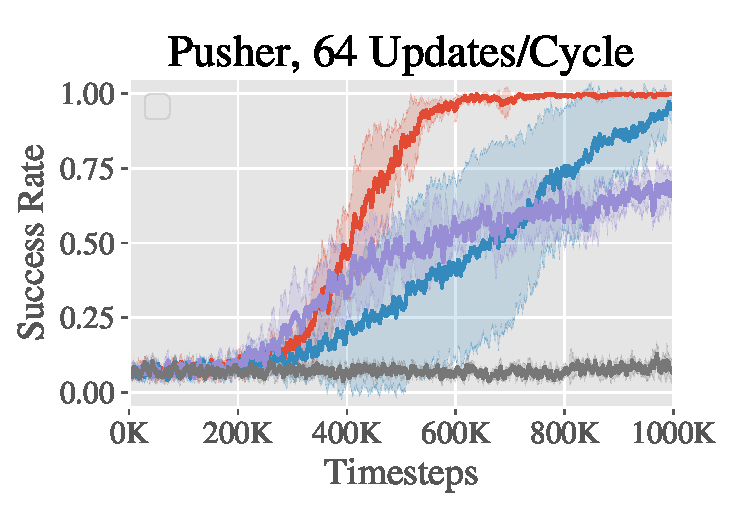
\includegraphics[height=0.2\linewidth]{img/her/push64.pdf}
    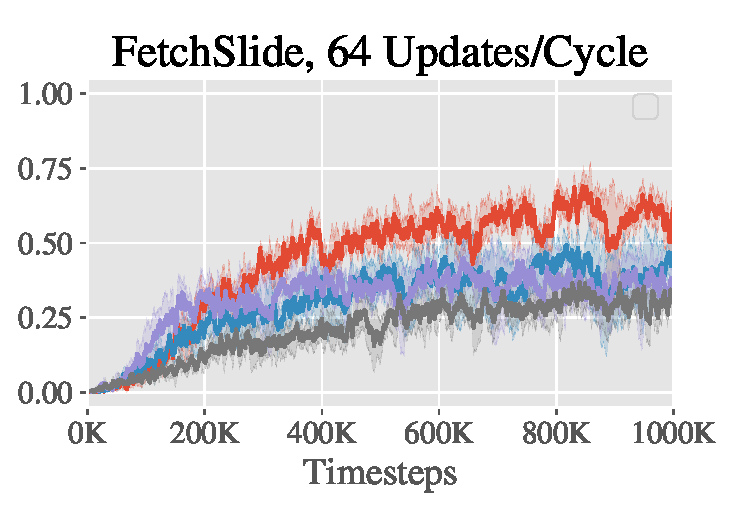
\includegraphics[height=0.2\linewidth]{img/her/slide64.pdf}
    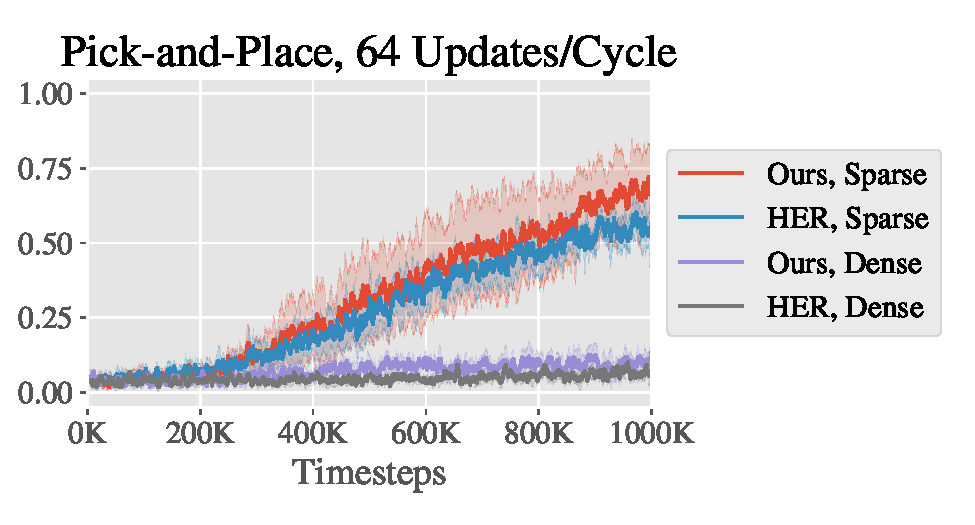
\includegraphics[height=0.2\linewidth]{img/her/pick64.pdf} \\
    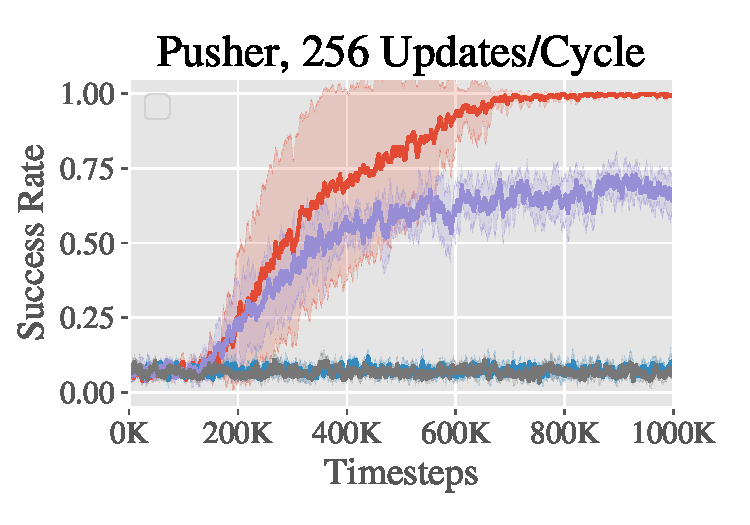
\includegraphics[height=0.2\linewidth]{img/her/push256.pdf}
    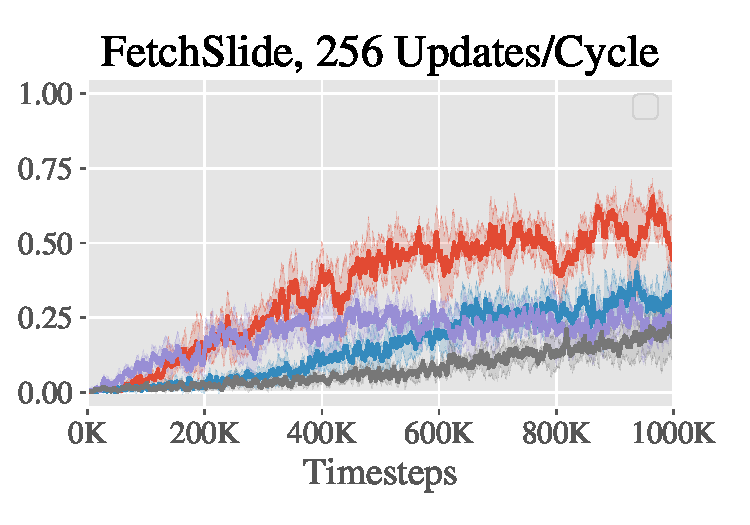
\includegraphics[height=0.2\linewidth]{img/her/slide256.pdf}
    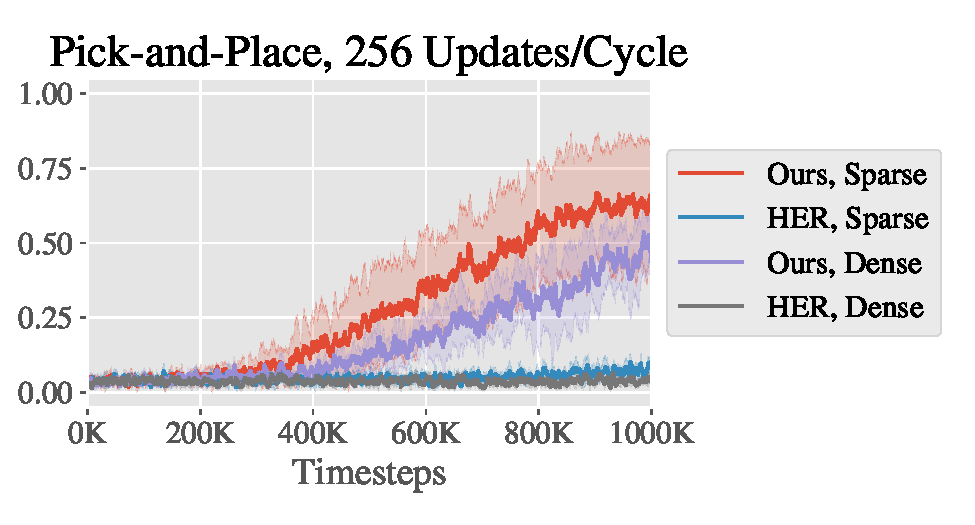
\includegraphics[height=0.2\linewidth]{img/her/pick256.pdf}
    \caption{Comparison between our relabeling strategy and HER. Each column shows a different task from the OpenAI Fetch robotics suite. The top row uses 64 gradient updates per training cycle and the bottom row uses 256 updates per cycle. Our relabeling strategy is significantly better  for both sparse and dense rewards, and for higher number of updates per cycle.}
    \vspace{-0.1in}
    \label{fig:her64}
\end{figure}

Results are shown in Figure \ref{fig:her64}. Our resampling strategy with sparse rewards consistently performs the best on the three tasks. Furthermore, it performs reasonably well with dense rewards, unlike HER alone which often fails with dense rewards. While the evaluation metric used here, success rate, is favorable to the sparse reward setting, learning with dense rewards is usually more sample efficient on most tasks and being able to do off-policy goal relabeling with dense rewards is important for RIG.

Finally, as the number of gradient updates per training cycle is increased, the performance of our strategy improves while HER does not improve and sometimes performs worse. As we apply reinforcement learning to real-world tasks, being able to reduce the required number of samples on hardware is one of the key bottlenecks. Increasing the number of gradient updates costs more compute but reduces the number of samples required to learn the tasks.

\section{Hyperparameters}
Table \ref{table:hyperparams} lists the hyperparameters used for the experiments.
\begin{table}[h]
\centering
\begin{tabular}{c|c|c}
\hline
\textbf{Hyperparameter} & \textbf{Value} & \textbf{Comments}\\
\hline
Mixture coefficient $\lambda$ & $0.5$ & See relabeling strategy ablation \\
\# training batches per time step & $4$ & Marginal improvements after $4$\\
Exploration Policy & OU, $\theta = 0.15, \sigma = 0.3$ & Outperformed Gaussian and $\epsilon$-greedy\\
$\beta$ for $\beta$-VAE & $5$ & Values around $[1, 10]$ were effective \\
Critic Learning Rate &$10^{-3}$ & Did not tune\\
Critic Regularization & None & Did not tune\\
Actor Learning Rate & $10^{-3}$ & Did not tune\\
Actor Regularization & None & Did not tune\\
Optimizer & Adam & Did not tune\\
Target Update Rate $(\tau)$ & $10^{-2}$ & Did not tune\\
Target Update Period & $2$ time steps & Did not tune\\
Target Policy Noise & $0.2$ & Did not tune\\
Target Policy Noise Clip & $0.5$ & Did not tune\\
Batch Size & $128$ & Did not tune\\
Discount Factor & $0.99$ & Did not tune\\
Reward Scaling & $10^{-4}$ & Did not tune\\
Normalized Observations & False & Did not tune\\
Gradient Clipping & False & Did not tune\\
% Critic FC sizes & False & Did not tune\\
\hline
\end{tabular}
\vspace{0.1cm}
\caption{Hyper-parameters used for all experiments.}
\label{table:hyperparams}
\end{table}

\section{Environment Details}
Below we provide a more detailed description of the simulated environments.

\textit{Visual Reacher}: A MuJoCo environment with a 7-DoF Sawyer arm reaching goal positions.
The arm is shown on the left of Figure \ref{fig:sim_screenshot} with two extra objects for the Visual Multi-Object Pusher environment (see below).
The end-effector (EE) is constrained to a 2-dimensional rectangle parallel to a table. 
The action controls EE velocity within a maximum velocity. 
The underlying state is the EE position $e$, and the underlying goal is to reach a desired EE position, $g_e$. 

\textit{Visual Pusher}: A MuJoCo environment with a 7-DoF Sawyer arm and a small puck on a table that the arm must push to a target push.
Control is the same as in Visual Reacher.
The underlying state is the EE position, $e$ and puck position $p$.
The underlying goal is for the EE to reach a desired position $g_e$ and the puck to reach a desired position $p$. 

\textit{Visual Multi-Object Pusher}: A copy of the Visual Pusher environment with two pucks.
The underlying state is the EE position, $e$ and puck positions $p_1$ and $p_2$.
The underlying goal is for the EE to reach desired position $g_e$ and the pucks to reach desired positions $g_1$ and $g_2$ respectively also constrained to each half of the workspace.
Each puck and respective goal is initialized in half of the workspace.

Videos of our method in simulated and real-world environments can be found at \url{https://sites.google.com/site/visualrlwithimaginedgoals/}.

\end{document}
